\documentclass[bachelor,nofonts,openright]{thuthesis}
%\documentclass[master]{thuthesis}
%\documentclass[doctor]{thuthesis}
% \documentclass[%
%   bachelor|master|doctor|postdoctor, % mandatory option
%   winfonts|nofonts|adobefonts, % mandatory only for bachelor and Linuxer
%   secret,
%   openany|openright,
%   arialtoc,arialtitle]{thuthesis}
% 当使用 XeLaTeX 编译时,本科生、Linux 用户需要加上 nofonts 选项;
% 当使用 PDFLaTeX 编译时,adobefonts 选项等效于 winfonts 选项(缺省选项)。

%%% figures
\usepackage[usenames,dvipsnames,svgnames,table]{xcolor}
\usepackage{pgf}
\usepackage{tikz}
\usepackage{tikz-timing}
  \usetikztiminglibrary{clockarrows}
  \usetikztiminglibrary{either}
  \usetikztiminglibrary{overlays}
  \tikztimingmetachar{b}[4] % b{lead-in}{text}{lead-out} for byte
    {#2D O{{[dotted]$(#1)-(#2)-(#4)$D{#3}}}{$(#1)-(#2)-(#4)$S} #4D}
\usepackage{caption}
\usepackage{subcaption}
\usepackage[export]{adjustbox}

%%% tables
\usepackage{booktabs}
\usepackage{tabularx}
\usepackage{longtable}
\usepackage{multirow}
\usepackage{diagbox}

%%% styles & symbols
\usepackage{lscape}
\usepackage{float}
\usepackage{rotating}
\usepackage{wasysym}
\usepackage{ulem}
\usepackage{xcolor}
\usepackage{verbatim}
\usepackage{newverbs}
  \newverbcommand{\cverb}{\color{red}}{}
  \newverbcommand{\bverb}
    {\begin{lrbox}{\verbbox}}
    {\end{lrbox}\colorbox{gray!30}{\box\verbbox}}
%\renewcommand{\emph}[1]{\CJKunderdot{#1}}
\usepackage{fontspec}
  \setmonofont{Consolas}
\newcommand{\csep}[0]{ -- } % intra-Caption SEParator

%%% AMS
\usepackage{amsmath}
\usepackage{amsfonts}
\usepackage{amssymb}

%%% physical
\usepackage{siunitx}
  \sisetup{
    retain-explicit-plus = true,
    per-mode = symbol,
    range-phrase = \ensuremath{\sim},
    range-units = single,
    list-units = single,
    binary-units = true
  }%
  \DeclareSIUnit \sccm{\ensuremath{\mathrm{sccm}}}
  \DeclareSIUnit \slm{\ensuremath{\mathrm{slm}}}
  \DeclareSIUnit \torr{\ensuremath{\mathrm{Torr}}}
\usepackage[version=3]{mhchem}



\begin{document}

% 定义所有的eps文件在 figures 子目录下
\graphicspath{{figures/}}


%%% 封面部分
\frontmatter
\ctitle{静电卡盘静电力检测装置设计与实现}

\makeatletter
\ifthu@bachelor\relax\else
  \ifthu@doctor
    \cdegree{工学博士}
  \else
    \ifthu@master
      \cdegree{工学硕士}
    \fi
  \fi
\fi
\makeatother


\cdepartment{机械工程系}
\cmajor{机械工程及自动化}
\cauthor{钟 音}
\csupervisor{程 嘉 副教授}

\etitle{Design and Implementation of Instrument for Measuring Electrostatic Force of Electrostatic Chucks}
\edegree{Bachelor of Engineering} 
\emajor{Mechanical Engineering and Automation}
\eauthor{Zhong Yin}
\esupervisor{Associate Professor Cheng Jia}

% 定义中英文摘要和关键字
\begin{cabstract}
IC产业是国家现代工业的基础,发展IC产业需要大量IC专用装备。静电卡盘是各类IC装备中重要的通用组件,广泛用于晶圆的夹持、搬运、以及工艺腔室中,其主要工作原理为通过在静电电极上加高电压,产生均匀分布的静电力将晶圆吸附在其表面陶瓷介电层上。静电力大小是静电卡盘最主要的性能指标,其大小及均匀程度直接影响晶圆温度大小与分布、平面度等其他性能指标,是设计优化的主要目标之一;但其产生机理复杂,理论和仿真模型均较难预测,需通过实验方法检测。

已有的静电力检测方案中具有多种影响其检测准确性与可重复性的因素,其中包括晶圆与静电卡盘间的间隙扩大、脱附过程自身的复杂性等等。为了更准确地检测静电力,本文针对已有方案中较为准确的背吹平衡方案中存在的问题提出了三点改进措施:检测环境为大气或真空(无等离子体)、引入微力探头组件以控制间隙并准确检测脱附、以及利用晶圆自重标定背吹等效面积,形成了新的检测方案。以此为基础,本文提出了采用新方案的检测平台的总体设计,将其分为微力探头组件、背吹控制系统、机械结构、以及自动控制与数据采集系统这四个组成子系统,并按照自顶向下的顺序给出了其中每一个组件的具体设计与选型等,完成了检测平台的设计方案。将方案中所有组件具体实现后,逐步完成了检测平台的组装、调试与搭建。

为验证检测方案以及检测平台确实能有效检测静电力,在检测平台上设计了静电力检测试验:通过前期试验找到了一些试验流程与方法中存在的不足之处,在提出了改进思路后,详细规划并完成了正式试验,获得了一系列微力探头受力与背吹压强的数据。之后,本文讨论了数据的处理与分析过程:将数据曲线按照特征分类,并通过对其反映的晶圆脱附物理过程的合理推测,总结出了较为系统的脱附点与脱附压强判定方法。经对正式试验数据的处理、分析、汇总与拟合,发现背吹压强与电极电压的关系较好地符合二次多项式,验证了检测方案与检测平台的可行性。
\end{cabstract}

\ckeywords{静电卡盘, 静电力, 脱附, 检测}

\begin{eabstract}
Semiconductor fabrication industry relies on many specialized devices. Electrostatic chucks (ESCs) are an important component commonly employed in these devices for holding silicon wafers both in transit and within process chambers. An ESC works by applying high electrostatic voltage across its electrodes, which produces evenly distributed electrostatic attractive force on the wafer, firmly chucking it to the surface of the ESC. Magnitude of total electrostatic force generated is the main specification of an ESC, having influence over other specifications such as wafer temperature distribution and flatness, thus being a main objective of design optimization. As the mechanism of electrostatic force generation is too complex for theoretical and simulation models, actual measurement is needed to evaluate the performance of an ESC.

Existing force measurement schemes exhibit poor repeatability and accuracy in measurement due to many factors such as the increase of gap between wafer and ESC surface during de-chucking, as well as the intrinsic complexity of the de-chucking process itself. In order to improve overall accuracy for force measurement, we proposed the following improvements over backside-pressure-balanced force measurement scheme: placing the ESC -- wafer system within atmosphere while allowing for vacuum (no plasma), using a force-sensitive probe for better de-chucking detection and eliminating influence of gap increase, and calibrating the equivalent acting surface area for wafer backside pressure. These led to our new force measurement scheme, based on which we designed and implemented a measurement platform using a top-down approach.

In order to evaluate the performance of the new measurement scheme and platform, we designed and conducted two stages of actual measurement experiments, first of which intended for finding out problems within platform implementation and experiment design, leading to the second stage which yielded a large amount of data. We then developed a systematic approach of interpreting and processing probe force -- backside pressure ($F$ -- $p$) curves, identifying the characteristic de-chucking point and associated de-chucking pressure from each curve measured. After processing all data curves, we aggregated the data on a de-chucking pressure -- electrode voltage plot, and found a good quadratic polynomial fit for the data, which verified our measurement scheme and platform.
\end{eabstract}

\ekeywords{Electrostatic Chuck, Electrostatic Force, Dechucking, Measurement}

% 设置 PDF 文档的作者、主题等属性
\makeatletter
\thu@setup@pdfinfo
\makeatother
\makecover

% 目录
\tableofcontents

% 符号对照表
\begin{denotation}

\item[ESC] 静电卡盘 (Electrostatic Chuck)
\item[wafer] 晶圆
\item[CFD] 计算流体力学 (Computational Fluid Dynamics)
\item[MFC] 质量流量控制器 (Mass Flow Controller)
\item[MCU] 微控制器单元 (Micro Controller Unit)
\item[ADC] 模数转换器 (Analog to Digital Converter)
\item[DAC] 数模转换器 (Digital to Analog Converter)


\end{denotation}


%manually fix \cleardoublepage if necessary
%http://sumanta679.wordpress.com/2009/07/02/latex-start-chapter-in-odd-page-in-case-cleardoublepage-not-working/
\begin{comment}
\newpage
\thispagestyle{empty}
\mbox{}
\end{comment}



%%% 正文部分
\mainmatter

\nocite{*}
% !TeX root = ../main.tex
\cleardoublepage
\chapter{引言}\label{ch:bg}



\section{课题背景}

%TODO: citation


\subsection{IC产业}

IC产业是一个国家现代工业的基础,是信息产业的核心,因此发展具有战略意义的集成电路产业以占领科技、经济和军事制高点已经成为许多国家的共识。

工信部发布的《集成电路产业“十二五”发展规划》中提出,到“十二五”末,集成电路产量超过1500亿块,销售收入达3300亿元,年均增长18\%,占世界集成电路市场份额15\%左右,满足国内近30\%的市场需求。

IC制造需要大量高技术制造装备;整个IC产业的迅速发展,也带动了IC装备制造业的发展。其中,关键制造装备的国产化是大势所趋。

IC制造工艺可分为四大类:沉积(deposition),去除(removal),布线(patterning),改性(modification of electrical properties)。常见的工艺包括PVD/CVD(物理/化学气相沉积)、等离子体刻蚀、化学机械平整化、旋转涂覆、光刻、离子移植、快速退火等。从单晶硅制成的晶圆,到最后的成品芯片,要依次经历多达300道工序。所有的IC工艺均需在严格受控的条件下进行,这需要专用设备的支持。


\subsection{静电卡盘}\label{sec:intro-echuck}

卡盘(chuck)是IC装备中的通用组件,用于夹取、搬运、或固定晶圆(wafer)及其他薄片类工件(如光刻掩模等)。依据其夹紧原理,主要可分为机械卡盘、真空吸盘和静电卡盘三种。机械卡盘需与工件保持紧固的机械接触,适用于要求不高或需要传动的场合,如搬运、旋转涂覆等;真空吸盘必须工作在大气环境下,与工件接触力极小,最适合用于搬运;静电卡盘结构、原理均复杂,但吸附力均匀稳定,且能满足各类工艺所需的额外要求,广泛用于工艺装备中。

\begin{figure}[hbt]
\centering
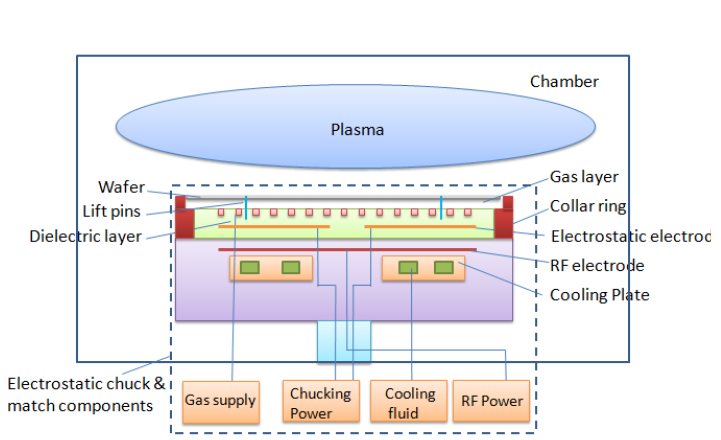
\includegraphics[width=1\linewidth]{./bg/echuck__sch.png}
\caption{静电卡盘组成示意}
\label{fig:echuck__sch}
\end{figure}

静电卡盘(如图~\ref{fig:echuck__sch})。



\section{国内外研究现状}

国内相关研究极其缺乏,在各文献数据库中均未搜索到静电卡盘静电吸引力测量的相关成果。其他静电卡盘相关的成果多为企业专利等,用于保护其独创设计。相对来说,国外对此有一定数量的研究,主要集中于静电吸附力产生机理、理论公式推导、定性实验验证、静电卡盘与工件组成系统的电学等效模型等方面。以静电力为重点的研究并不多,多数文章仅对“测量静电力”一笔带过,并未深入探究其测量手段。


\subsection{主要研究机构与企业}


\subsection{主要测量手段概述}\label{sec:priorArt}

\subsubsection{机械提拉法}\label{sec:priorArt-pull}
\subsubsection{背吹平衡法}\label{sec:priorArt-backside}
\subsubsection{变形检测法}\label{sec:priorArt-warp}



\section{论文研究内容与意义}


\subsection{工程需求}


\subsection{论文研究内容}


\subsection{对专项课题的推进作用}
% !TeX root = ../main.tex
\cleardoublepage
\chapter{检测原理与方案设计}\label{ch:principle}



\section{背吹平衡法原理分析}\label{sec:principle-backside}


\subsection{受力分析}\label{sec:principle-backside-force}

\begin{figure}[tbh]
\centering
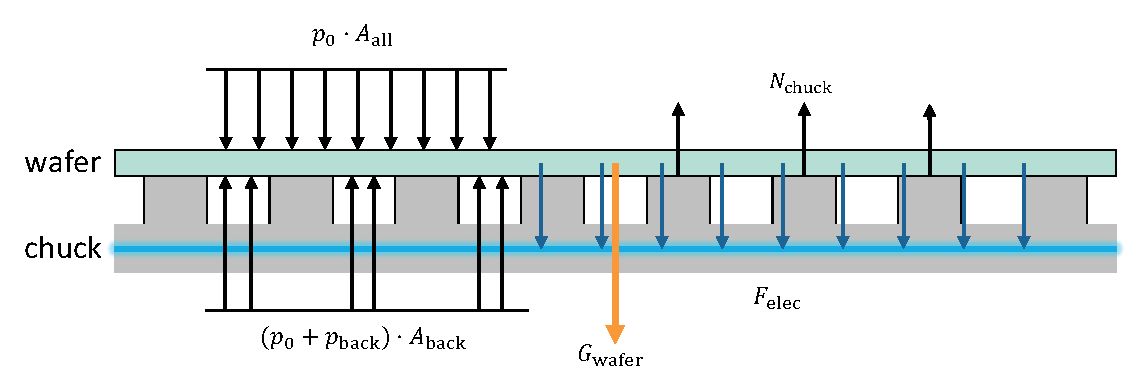
\includegraphics[width=1\linewidth]{principle/force__orig}
\caption{背吹平衡法中晶圆受力分析}
\label{fig:principle-backside-force}
\end{figure}

当静电卡盘处于正常工作状态时,晶圆牢固吸附在静电卡盘表面,其受力情况如图~\ref{fig:principle-backside-force},处于平衡状态,有:
\begin{equation}
\label{eq:principle-backside-force}
(p_{0} + p_{\mathrm{back}}) \cdot A_{\mathrm{back}} + N_{\mathrm{chuck}} = p_0 \cdot A_{\mathrm{all}} + G_{\mathrm{wafer}} + F_{\mathrm{elec}}
\end{equation}
其中:
\begin{itemize}
  \item $p_{0}$ : 环境压强(绝对)
  \item $p_{\mathrm{back}}$  : 背吹压强(相对于$p_{0}$)
  \item $A_{\mathrm{back}}$  : 晶圆背面气压等效作用面积(见\ref{principle-prob-area}节)
  \item $A_{\mathrm{all}}$   : 晶圆总面积
  \item $N_{\mathrm{chuck}}$ : 静电卡盘表面向晶圆提供的总支持力
  \item $G_{\mathrm{wafer}}$ : 晶圆总重力
  \item $F_{\mathrm{elec}}$  : 晶圆所受总静电吸引力
\end{itemize}
当晶圆即将脱附时,有 $N_{\mathrm{chuck}} \to 0$ ;此时 \eqref{eq:principle-backside-force} 可近似为:
\[
(p_{0} + p_{\mathrm{back}}) \cdot A_{\mathrm{back}} = p_0 \cdot A_{\mathrm{all}} + G_{\mathrm{wafer}} + F_{\mathrm{elec}}
\]
即:
\begin{equation}
\label{eq:principle-backside-force-derived}
F_{\mathrm{elec}} = (p_{0} + p_{\mathrm{back}}) \cdot A_{\mathrm{back}} - p_0 \cdot A_{\mathrm{all}} - G_{\mathrm{wafer}}
\end{equation}

虽然分析时将重力与支持力简化等效为集中力,实际上晶圆受到的包括重力与支持力在内的所有力均为分布力。因此,若假设静电力分布足够均匀,上述分析同样适用于晶圆局部。


\subsection{脱附条件}\label{sec:principle-backside-dechuck}

背吹平衡法中,需人为产生并检测晶圆即将脱附至完全脱附的状态,从而间接获得静电力大小。制造脱附条件的基本方法是使背吹压力相对于静电吸引力更大,可通过提高气压、降低电压等方式实现。检测脱附的基本方法是监测晶圆在脱附时产生变化的物理量,如位移(晶圆挠度)、电极电压/电流、背吹压强/流量等。%TODO:analysis/xref



\clearpage



\section{背吹平衡法中存在的问题}\label{sec:principle-prob}


\subsection{工作环境}\label{sec:principle-prob-env}

静电卡盘常见于工艺腔室中,其内部为真空或绝对压强极低的等离子体(单极型静电卡盘必须在等离子体存在的环境中才能工作)。已有检测方案大多设计为在真空条件、甚至等离子体条件下工作,以复现实际工艺条件。虽然这样可能有助于提高测试结果的准确度,但在真空与等离子体条件下试验存在如下问题:无论等离子存在与否,均需围绕选定的静电卡盘及检测仪器等设计并搭建专真空腔室,系统组成极为复杂,难度与刻蚀机核心部分设计相当。即使已有合适的腔室与配套设备,在开始检测之前,需等待真空泵将腔室抽成真空,时间长达数小时,而一旦需打开腔室进行调整,必须在此之前平衡气压,调整后再花费数小时抽真空,效率极低。此外,当等离子体存在时,晶圆上方大部分空间无法放置任何物体,以避免等离子体受到遮挡或与异物产生相互作用;这对测量系统的设计是过于苛刻的约束条件。


\subsection{间隙与部分脱附}\label{principle-prob-gap}

已有脱附试验(包括但不限于背吹平衡法)中存在一个共有问题:当\emph{检测}到脱附时,晶圆实际已部分脱附,即脱附是一连续变化的过程
%TODO:cite 曹明路
;此时晶圆与卡盘的间隙大于未脱附(正常工作)时,而根据\eqref{eq:bg-coulomb}式,静电力随着间隙扩大急剧下降,导致测得的静电力一定小于工作状态静电力,即测量存在较大系统误差。如能设法减小该误差,则可提高测量的准确度。

误差的消除需要更好的脱附检测手段。虽然瞬态过程(如晶圆突然出现明显脱附等)容易检测且不易误判,但此时晶圆并非处于平衡态,且其在微观上可能已大部分脱附,加上检测仪器的响应延迟(精度较高的仪器往往延迟也更大),对系统误差影响极大。为避免瞬态过程带来的系统误差,应维持系统处于准静态或缓变过程中。然后,为了减小部分脱附对检测产生的影响,需快速、准确地判定刚刚开始脱附这一现象;此时间隙未明显扩大,静电力相对于工作状态未出现明显偏差,即减小了系统误差。为此,需选取合适的脱附特征物理量,并设计对应检测手段,改进脱附判定。


\subsection{背吹通道流动}\label{sec:principle-prob-flow}

已有背吹平衡方案均假定晶圆背面受均匀压强作用,但未论证该假设的合理性:背吹通道中存在的流动是否会影响晶圆背面受力情况?若有,则检测准确度可能会受到影响。因此,有必要分析晶圆背面的流动情况。

\subsubsection{建立CFD模型}\label{sec:principle-prob-flow-cfd-setup}

为了方便后续仿真工作的开展,此处选择Comsol作为仿真软件;先搭建简化模型,做出基本判断,再根据后续试验需要,进一步添加细节,提高仿真准确度。

\begin{figure}[tbh]
\centering
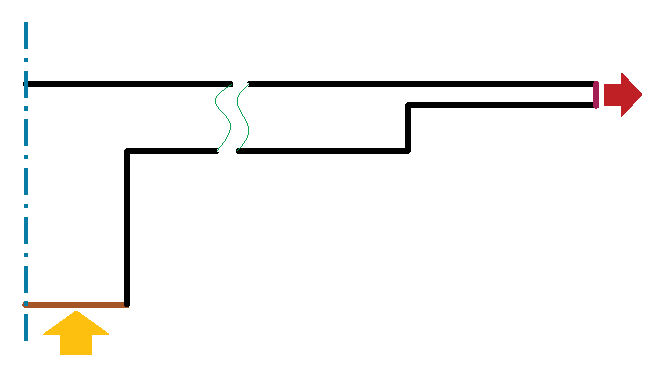
\includegraphics[width=0.72\linewidth]{principle/cfd__setup}
\caption{晶圆背面流动CFD建模示意}
\label{fig:principle-flow-cfd-setup}
\end{figure}

由待测静电卡盘\footnote{具体参数见\ref{sec:rig-overall}节。}背吹通道特点知,流动主要为平板间层流,因此选用层流模块(\bverb|spf|)求解。几何模型选用二维轴对称(2D Axisymmetric,即纯旋转体),流道截面如图~\ref{fig:principle-flow-cfd-setup}\footnotemark{};在正中间设一圆柱形进气口,直径\SI{1}{\mm},固定其压力为\SI{2}{\kPa}表压;在边缘处用均匀圆环形狭缝来等效晶圆与陶瓷介电层的接触密封,外侧设为出口,固定为大气压。

\footnotetext{此处流道宽度由陶瓷介电层表面的凸台高度决定,但为了简化分析起见,暂时忽略凸台影响。}

由于目前对接触密封的了解尚少,无法准确估计等效狭缝宽度,因此设定参数扫描,求解当狭缝宽度为\SIrange{1}{0.1}{\um}(\bverb|10^{range(0,-1/2,-1)}[um]|)时的流动情况。

\subsubsection{CFD仿真结果}\label{sec:principle-prob-flow-cfd-result}

当狭缝宽度改变时,速度场变化不大,最大速度均出现在进口附近,之后速度迅速衰减至稳定,如图~\ref{fig:principle-flow-cfd-result-vel} 。

%TODO:动量呢?

在入口处对$v_z\ \rho$取面积分,得到质量流量如表\ref{tab:principle-flow-cfd-result-flow}。单位\si{\mg\per\minute}大致与sccm相当,即质量流量在狭缝宽\SI{1}{\um}时,仍低于1 sccm;狭缝变窄时,流量得非常快。这说明只要密封处的实际表面粗糙度足够低,接触足够紧密,则气体泄漏几乎可忽略不计;若安装流量计,则应选取较小量程的型号(一般为10 sccm)。

沿模型上边界(即晶圆下表面)绘制压强 -- 半径曲线,如图~\ref{fig:principle-flow-cfd-result-pressure} ,发现在流道中段压降满足$\Delta p \propto \log{r}$。 %TODO:derive by hand
当狭缝宽\SI{1}{\um}时,在中段存在明显压降(约\SI{0.6}{\kPa}),显然\textbf{不能忽略};但当狭缝更窄时,压降迅速衰减,当狭缝宽\SI{0.3}{\um}时已可忽略。当然,这是假定只有卡盘中央有一个气孔的时候的情形,而实际的静电卡盘为了控制温度分布均匀,在整个表面多处分布气孔,可使压强分布更均匀。即便如此,在处理实验数据时,应小心验证压强分布(可进一步构建三维流道模型以得到更准确的仿真数据),不能直接认为晶圆受均匀气压作用。

\begin{table*}[thbp]
\centering
\caption{CFD仿真结果\csep 进口处质量流量}
\label{tab:principle-flow-cfd-result-flow}
\begin{tabular}{SS}
  \toprule[1.5pt]
  狭缝宽度/\si{\mm}  &  质量流量/\si{\mg\per\minute}  \\
  \midrule[1pt]
  \num{1.000}  &  \num{2.183e-1}  \\
  \num{0.316}  &  \num{9.628e-3}  \\
  \num{0.100}  &  \num{3.079e-4}  \\
  \bottomrule[1.5pt]
\end{tabular}
\end{table*}

\begin{figure}[hbp]
\centering
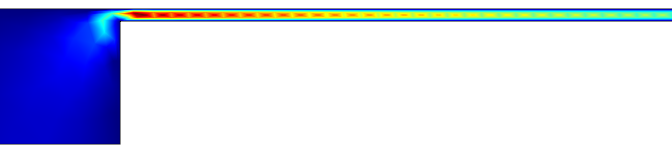
\includegraphics[width=0.72\linewidth]{principle/cfd__vel.png}
\caption[CFD结果:速度场]{CFD仿真结果:进口附近速度场}
\label{fig:principle-flow-cfd-result-vel}
\end{figure}

\begin{figure}[hbp]
\centering
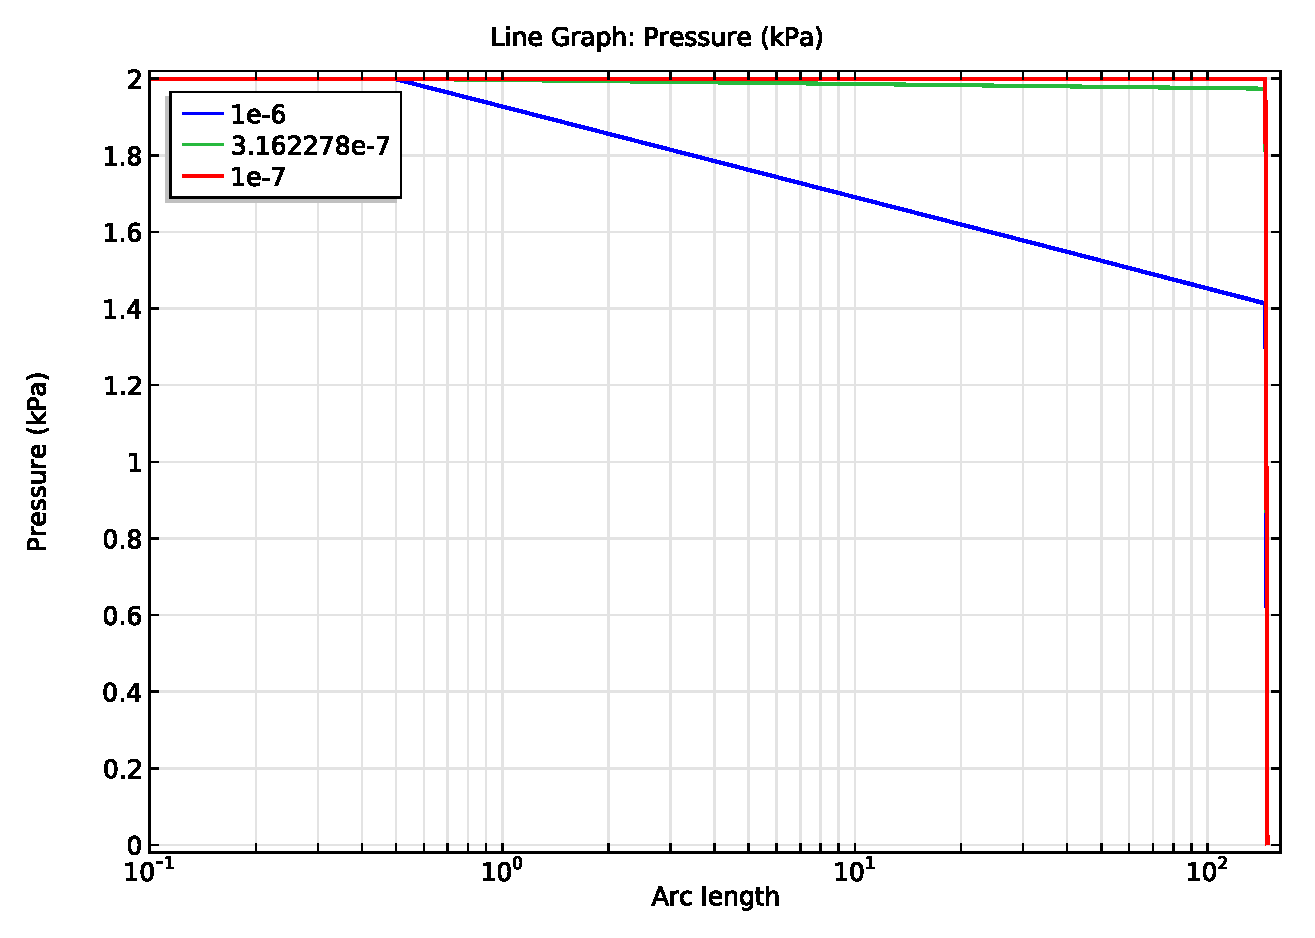
\includegraphics[width=1\linewidth]{principle/cfd__pressure}
\caption{CFD仿真结果\csep 压力沿径向分布}
\label{fig:principle-flow-cfd-result-pressure}
\end{figure}


\clearpage


\subsection{压强等效作用面积}\label{principle-prob-area}

\eqref{eq:principle-backside-force}式中,晶圆背面气压等效作用面积(即$A_{\mathrm{back}}$)是未知量。
%TODO:cite nagoya
由于陶瓷介电层上的凸台高度较低(约\SI{10}{\um})与晶圆背面接触情况不明,尚不能直接断言$A_{\mathrm{back}}$等于晶圆背面所有未与陶瓷层凸台/边缘接触部分的面积。由于此处无法用普通CFD求解,需要设计额外的标定步骤,测出$A_{\mathrm{back}}$数值。



\section{改进方案设计}\label{principle-soln}


\subsection{工作环境}\label{principle-soln-env}

由\ref{sec:principle-prob-env}节中讨论,真空与等离子体环境均不利于检测系统的设计、实现与使用,因此改进方案为在大气环境下使用设计,并可在不改变主要原理的条件下,经过尽可能少的修改,移植到真空腔室中;等离子体环境不予考虑。


\subsection{引入微力探头判定脱附}\label{principle-soln-ruby}

\begin{figure}[tbhp]
\centering
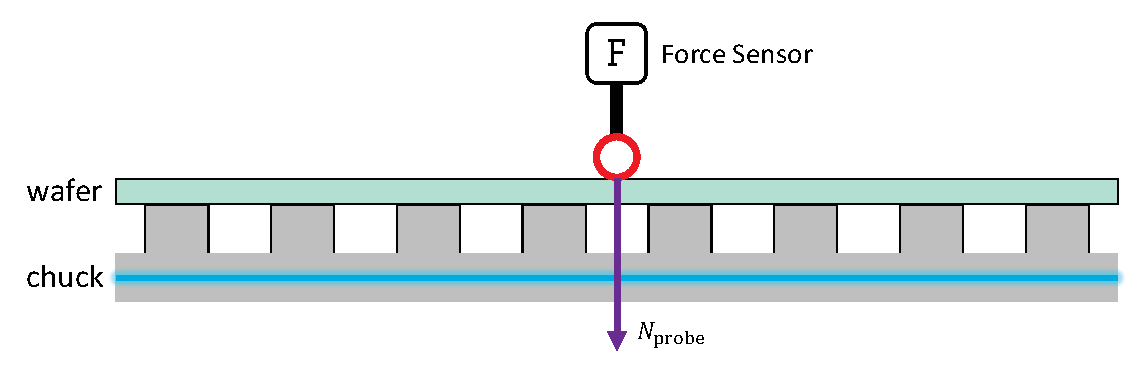
\includegraphics[width=1\linewidth]{principle/soln__ruby__sch}
\caption{微力探头原理示意}
\label{fig:principle-soln-ruby-sch}
\end{figure}

考虑\ref{sec:principle-backside-force}节中的受力平衡关系。虽然在即将脱附时,$N_{\mathrm{chuck}} \to 0$,但此时存在\ref{principle-prob-gap}节中阐述的间隙扩大问题。如果希望抑制间隙扩大,则必须向晶圆施加一个向下的力$N'$。注意即使晶圆在即将脱附时,其在$N'$作用下仍处于平衡状态,且力平衡方程变为:
\begin{equation}
\label{eq:principle-soln-ruby-force}
(p_{0} + p_{\mathrm{back}}) \cdot A_{\mathrm{back}} + N_{\mathrm{chuck}} = p_0 \cdot A_{\mathrm{all}} + G_{\mathrm{wafer}} + F_{\mathrm{elec}} + \mathbf{N'}
\end{equation}
若$N'$大小可测量,则可将其作为脱附特征物理量,准确判定部分脱附。据此设计微力探头,如图~\ref{fig:principle-soln-ruby-sch},其组成为一单轴微力传感器以及连接在其上的标准三坐标测量机红宝石探头(图中以红色圆形表示,实际为球体)。晶圆吸附后,使红宝石探头与已吸附的晶圆表面接触,探头方向垂直于晶圆表面,则由牛顿第三定律,传感器受到的压缩力和探头施加在晶圆上的支持力$N_{\mathrm{probe}}$大小相等\footnotemark{};若采取措施确保此时$N_{\mathrm{probe}} \ll F_{\mathrm{elec}}$,则可认为$N_{\mathrm{probe}} \approx 0$。逐渐增加背吹气压,直至晶圆脱附这一过程中,$N_{\mathrm{chuck}} \to 0$,并逐渐转由探头向晶圆提供支持力,即$N_{\mathrm{probe}}$明显增加,可作为判定晶圆开始脱附的根据。由于传感器自身具有一定弹性(在量程范围内可等效为一理想弹簧),晶圆在与探头接触的一点仍有一定挠度,但由胡克定律$F = k x$知,该点挠度可由测得的$N_{\mathrm{probe}}$和传感器刚度$k$计算出,并且对于给定传感器,$k$已知,而$N_{\mathrm{probe}}$可人为地在传感器量程内选取有效取值区间,因此在判定脱附时,该挠度也处于一个确定的取值区间内,即晶圆与卡盘的间隙得到了控制。

\footnotetext{即为上文$N'$;另外,下文中不再区分这一对反作用力,仅用$N_{\mathrm{probe}}$表示其大小。}


\subsection{晶圆自重平衡法求压强等效面积}\label{sec:principle-soln-gravity}

\begin{figure}[tbhp]
\centering
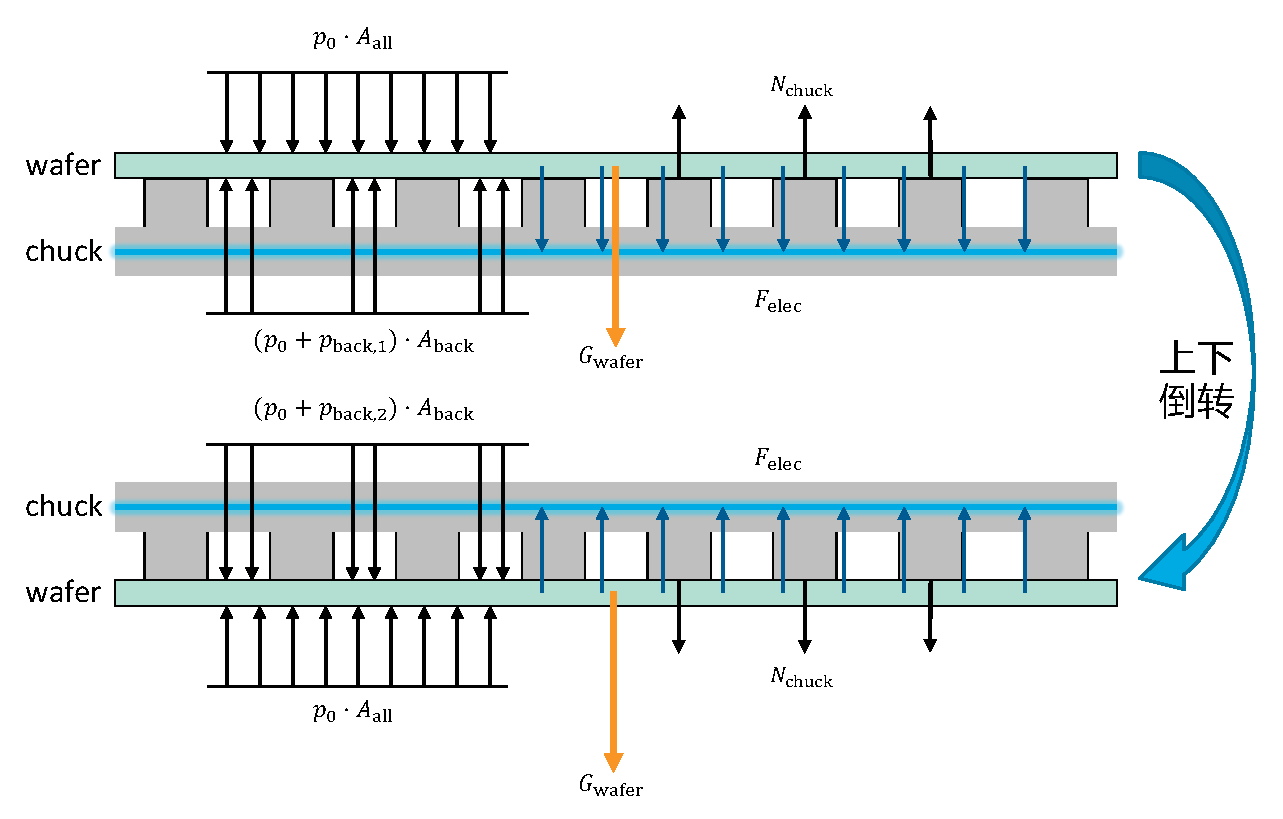
\includegraphics[width=1\linewidth]{principle/area__gravity__sch}
\caption{晶圆自重平衡法求压强等效作用面积示意}
\label{fig:principle-area-gravity-sch}
\end{figure}

建立一个固连在静电卡盘上的坐标系,注意到在晶圆受力平衡关系中,除重力以外,其他力相对于该坐标系的方向均固定,而重力方向随着静电卡盘姿态改变而改变。若将静电卡盘上下倒转\ang{180},则相对于静电卡盘坐标系,只有晶圆受到的重力方向反转。据此可求出压强等效面积:分别在试验台正放和倒放两种状态下,加相同电压,完成背吹平衡试验,得到即将脱附时的背吹压强分别为$p_{\mathrm{back},1}$和$p_{\mathrm{back},2}$(可通过多次测量取平均值的方法来减小随机误差)。根据受力平衡关系有:
\begin{equation}
\label{eq:principle-area-gravity-orig}
\begin{aligned}
(p_{0} + p_{\mathrm{back},1}) \cdot A_{\mathrm{back}} & = p_0 \cdot A_{\mathrm{all}} + G_{\mathrm{wafer}} + F_{\mathrm{elec}} \\
(p_{0} + p_{\mathrm{back},2}) \cdot A_{\mathrm{back}} & = p_0 \cdot A_{\mathrm{all}} - G_{\mathrm{wafer}} + F_{\mathrm{elec}}
\end{aligned}
\end{equation}
两式相减:
\[
(p_{\mathrm{back},1} - p_{\mathrm{back},2}) \cdot A_{\mathrm{back}} = 2 G_{\mathrm{wafer}}
\]
即:
\begin{equation}
\label{eq:principle-area-gravity-derived}
A_{\mathrm{back}} = \frac{2 G_{\mathrm{wafer}}}{p_{\mathrm{back},1} - p_{\mathrm{back},2}}
\end{equation}
即求得$A_{\mathrm{back}}$数值。需要注意的是,$A_{\mathrm{back}}$可能与所加电压、晶圆材料、厚度等各种参数相关,可改变条件,多次试验,得出$A_{\mathrm{back}}$对各参数的敏感度。



\section{本章小结}\label{sec:principle-summary}

本章首先分析了原有背吹平衡法检测静电力的工作原理,指出了其中存在的影响测量准确性的因素,包括晶圆部分脱附、晶圆与静电卡盘间存在的间隙扩大、背吹通道流动对晶圆背面压强分布的影响、以及压强等效作用面积等,进而针对其中最主要的部分脱附、间隙、以及压强等效作用面积问题,提出微力探头、自重平衡两种措施作为改进方案,并阐明了其减小原有方案中误差的原理。

% !TeX root = ../main.tex
\chapter{检测平台设计}\label{ch:rig}

本章以上一章提出的改进方案为基础,讨论大气环境下的静电卡盘静电力检测平台的设计。由于检测平台是一个复杂的机、电、气相结合的系统,本章首先分析检测平台所需具有的功能与组成部分,然后提出其总体设计方案,最后分组件讨论检测平台各部分的具体设计。



\section{总体设计方案}\label{sec:rig-overall}

根据已有背吹平衡方案,以及\ref{principle-soln}节中提出的改进措施(主要是微力探头),确定检测平台必须具有的功能如下:对静电卡盘背吹通道气压的控制与检测、对微力探头的定位与受力检测、检测过程的自动控制、数据采集与储存等。据此,可将整个平台划分为图~\ref{fig:rig-overall-sch}~所示的几大组成部分:

\begin{figure}[tbh]
\centering
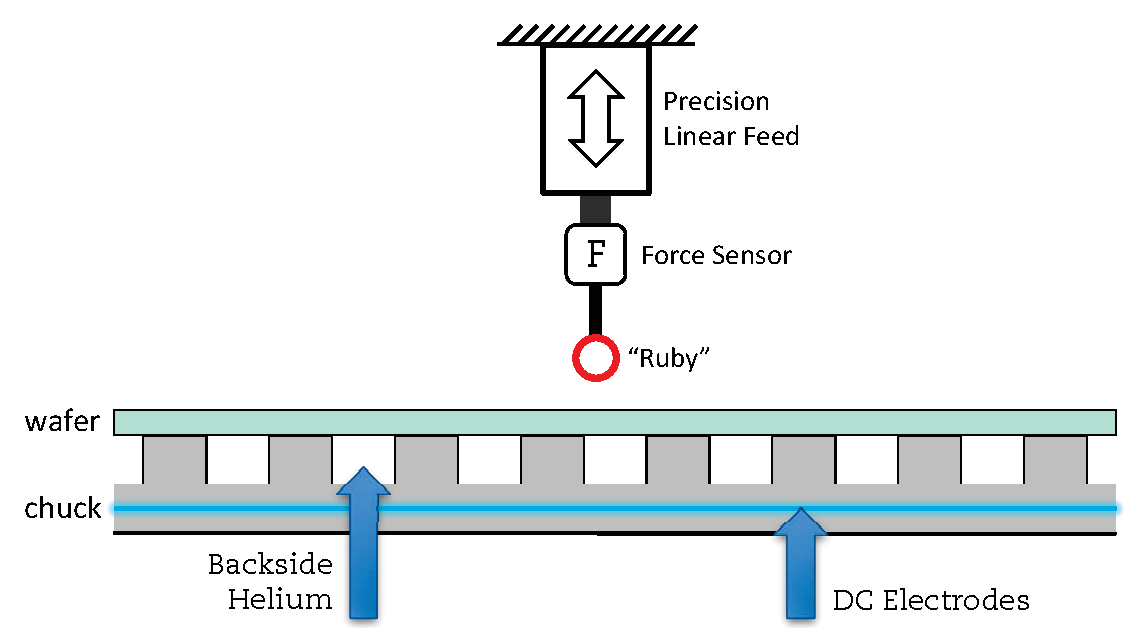
\includegraphics[width=1\linewidth]{rig/overall__sch}
\caption{测量平台总体设计方案示意}
\label{fig:rig-overall-sch}
\end{figure}

\begin{enumerate}
  \item \textbf{待测静电卡盘及其配套静电电源} :
    待测静电卡盘为北方微电子公司提供的一台\SI{300}{\mm}双极型静电卡盘,如图~\ref{fig:rig-overall-chuck},采用埋在氮化铝陶瓷层中的交叉环形金属电极。其陶瓷层表面均布圆形小凸台,边缘处有宽约\SI{2}{\mm}的环形凸起,共同形成背吹通道。配套的直流静电电源可通过标准接头与静电卡盘两电极相连,提供高达\SI{3000}{\V}的静电电压。
  \item \textbf{微力探头组件} :
    图~\ref{fig:rig-overall-sch}中位于卡盘上方的部分即为微力探头组件,其主体为\ref{principle-soln-ruby}节所述的微力探头。详细设计在\ref{sec:rig-probe}节讨论。
  \item \textbf{背吹控制系统} :
    向静电卡盘背吹通道提供稳定、可控的气压,并检测背吹通道入口处气压值。详细设计在\ref{sec:rig-pressure}节讨论。
  \item \textbf{机械结构} :
    为所有其他组件(包括配管配线等)提供定位、支撑作用。详细设计在\ref{sec:rig-model}节讨论。
  \item \textbf{自动控制与数据采集系统} :
    包括微力探头组件与背吹控制系统中的接口电路、总控单元、以及PC三大部分,主要功能为自动控制整个检测过程,采集各传感器数据,并将其传输到PC中储存。详细设计在\ref{sec:rig-ctrl}节讨论。
\end{enumerate}

\begin{figure}[p]
\centering
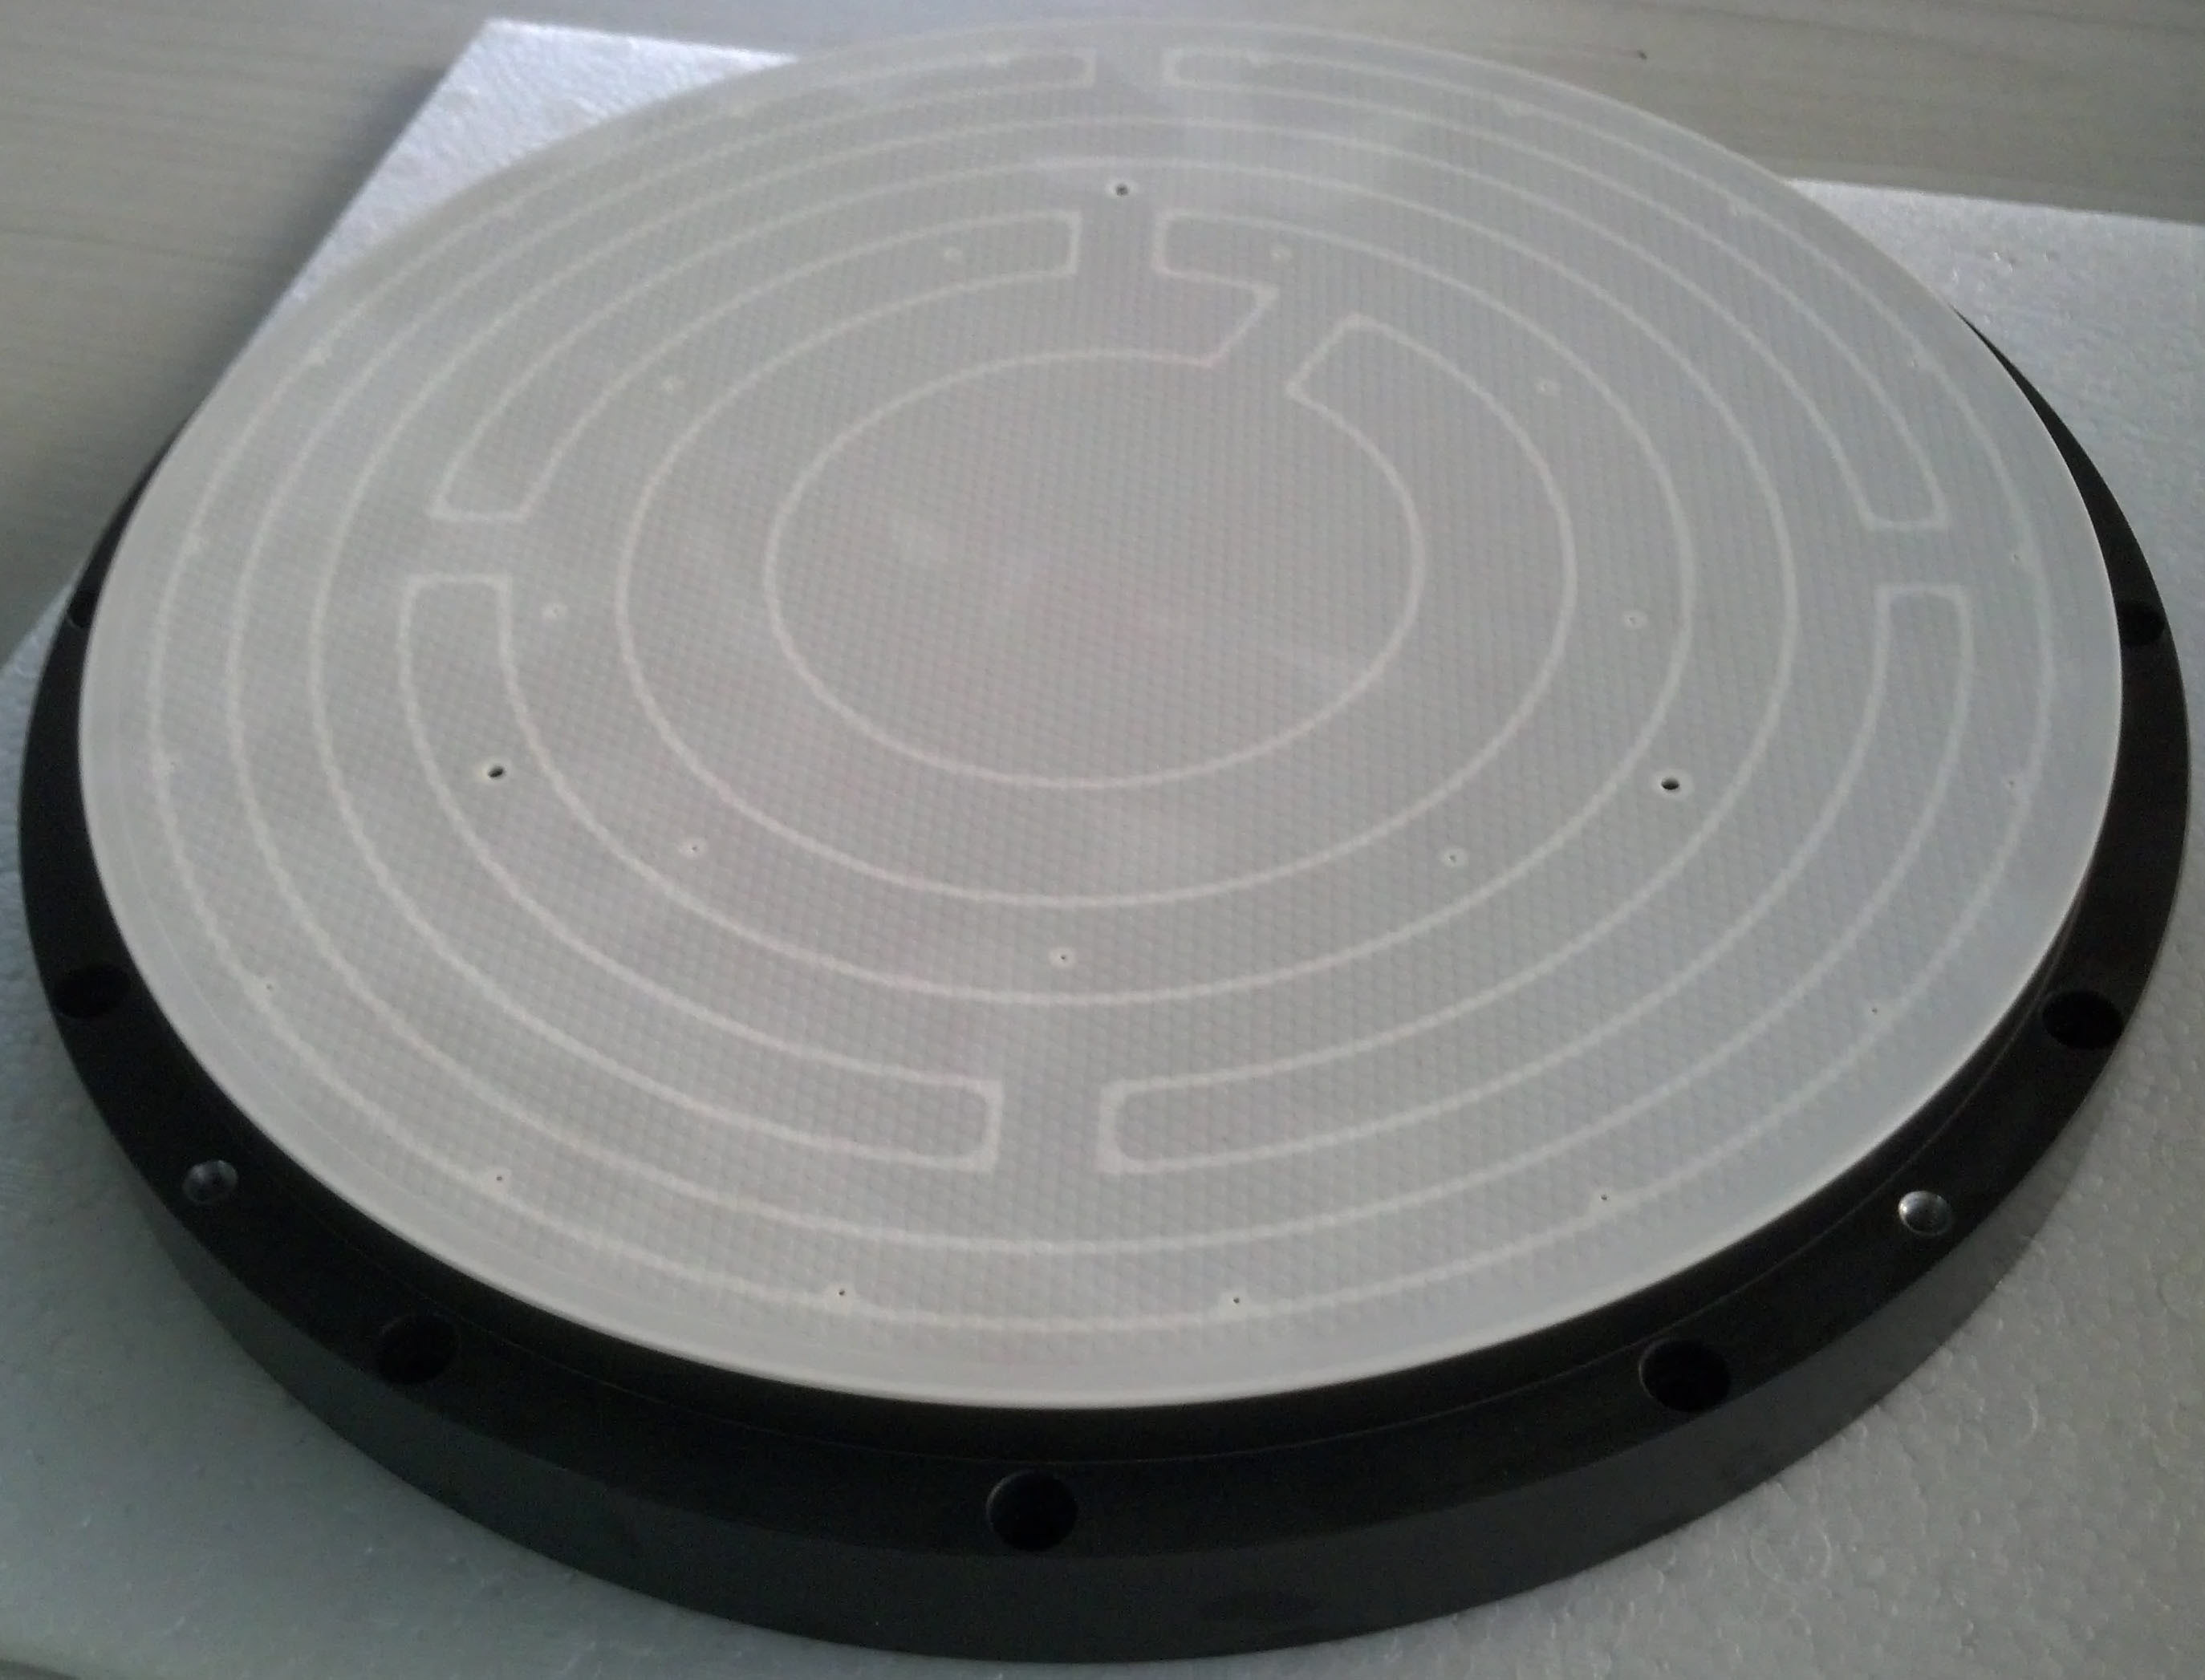
\includegraphics[height=0.40\textheight]{rig/overall__chuck__front.jpg} \\
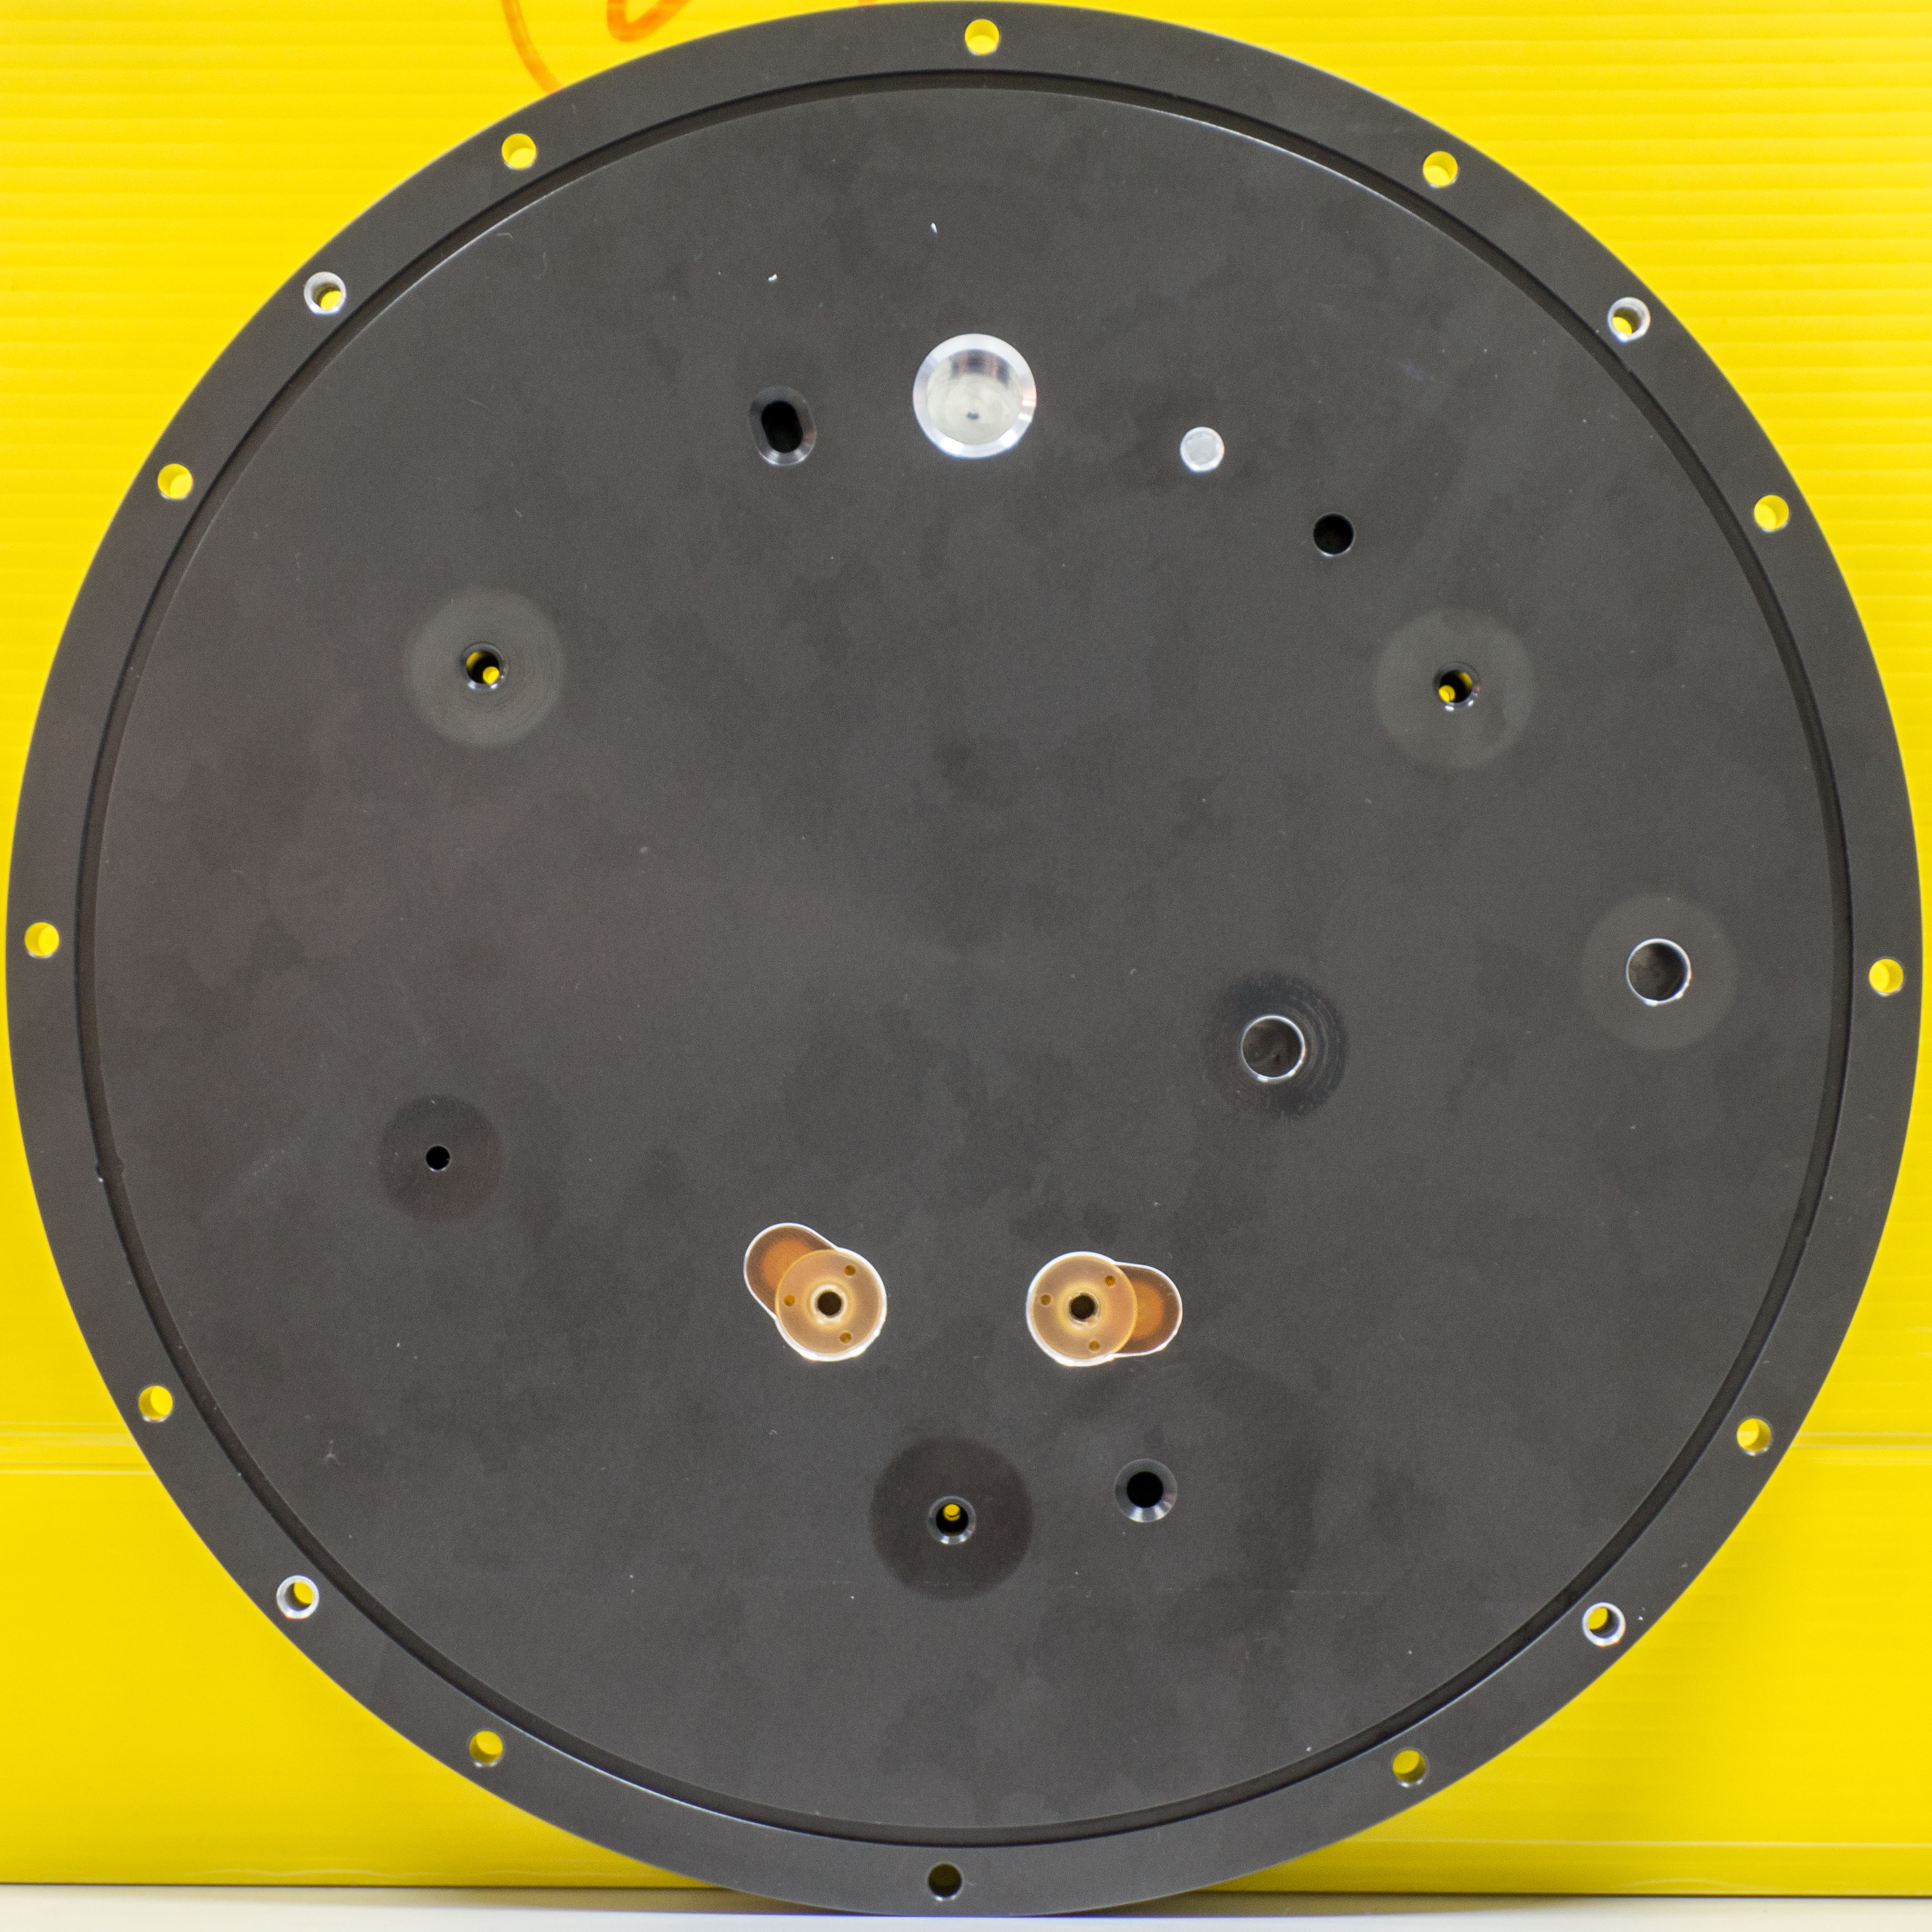
\includegraphics[height=0.50\textheight]{rig/overall__chuck__back.jpg}
\caption{待测静电卡盘}
\label{fig:rig-overall-chuck}
\end{figure}



\clearpage



\section{微力探头组件设计}\label{sec:rig-probe}

\ref{principle-soln-ruby}节中提出了由微力传感器和红宝石探头组成的微力探头。该探头需在晶圆吸附后与晶圆接触,并保证接触力$N_{\mathrm{probe}} \ll F_{\mathrm{elec}}$。这可通过增设精密直线进给机构实现。具体方法如下:将微力探头组件连接到进给机构的移动端,进给机构的固定端连接在检测平台框架上,如图~\ref{fig:rig-overall-sch}。晶圆吸附后,驱动进给机构向靠近晶圆方向缓缓移动,同时通过微力传感器监测$N_{\mathrm{probe}}$;当$N_{\mathrm{probe}}$测量值明显增加,超过一定阈值\footnotemark{}时,立即停止进给机构运动,则此时$N_{\mathrm{probe}}$大小由阈值、传感器刚度、进给速度、进给机构特性共同决定,只要参数选取合适,即可保证$N_{\mathrm{probe}} \ll F_{\mathrm{elec}}$。

\footnotetext{该阈值可人为根据传感器特性确定,也可通过数字信号处理方式动态获得,甚至可采用阈值判定以外的其他方式,在此不再赘述。}

微力探头组件中,红宝石探头可直接从标准三坐标测量机探头组中选取,而微力传感器与进给机构需外购。本节主要讨论两外购件的选型。


\subsection{微力传感器选型}\label{sec:rig-probe-sensor}

微力传感器是探头组件中的核心元件,由上文讨论知,其关键参数与系统性能直接相关,且影响进给机构的选型,因此需首先确定其选型。本节通过对检测过程的分析,先估测关键参数的范围,以此为标准筛选出备选产品,最后对比评估选择合适的微力传感器。

量程是微力传感器最主要的参数,所有相对性能指标均以满量程为基准,如精度、分辨力、敏感度等。合理的量程选择应完全覆盖传感器在整个检测过程中受力的范围,但又不超过该范围过多,以保证测量精度,减小噪声干扰。由于检测过程中需一直保证$N_{\mathrm{probe}} \ll F_{\mathrm{elec}}$,而保守估计静电力$F_{\mathrm{elec}}$在$\SIrange{5}{200}{\N}$范围内,若设定1\%作为“远小于”的上界(即$N_{\mathrm{probe}} \leq 0.01 \cdot F_{\mathrm{elec}}$),则$N_{\mathrm{probe}} \leq \SI{0.05}{\N}$,由此确定传感器量程合理取值范围为$\SIrange{0.05}{0.5}{\N}$。确定量程后,还需确定与其直接相关的安全过载范围。考虑到在安装、调试过程中,以及硅晶圆突然完全脱附时,探头均可能瞬间受到较大的力的作用,若微力传感器具有较大安全过载范围,则可避免意外受损。保守估计传感器需至少能承受\SI{0.5}{\N}量级的瞬间轴向压缩力而性能不受影响。

为了准确检测脱附,需要传感器能分辨较小的受力增量,即具有高分辨力。一般分辨力标称值为满量程的百分比(\% FS),在比较量程不同的传感器时,需先将其转换为绝对数值。当传感器未标称分辨力时,可参考其重复精度数据。由于传感器分辨力越高,成本也越高,根据静电力范围粗估\SI{0.25}{\mN}作为分辨力的参考数值。%TODO:more reasoning

另外,由\ref{principle-soln-ruby}节中关于晶圆挠度的讨论,在其他条件不变的情况下,传感器刚度$k$越高,晶圆挠度范围越小,但同时越难控制探头与晶圆的初始接触力(见上文中保证接触力方法,以及\ref{sec:rig-probe-feeding}节\eqref{eq:rig-probe-feeding-vel}式)。因此,挠度取值及其对检测的影响需作为选型时的重要参考。

表~\ref{tab:rig-probe-sensor}为初步筛选后的选型表。若考虑量程、精度、分辨力,1050V1较差;若考虑刚度,LSB200较差;若考虑过载性能,FT-S10000较差。综合考虑,LSB200在量程、过载范围、重复精度等方面与预期符合最好,因此选择该产品。

% generated using http://www.tablesgenerator.com/latex_tables
\begin{table}[htbp]
\begin{minipage}{1\linewidth}
\centering
\caption{微力传感器选型表}
\label{tab:rig-probe-sensor}
\begin{tabular}{@{}lllccc@{}}
\toprule[1.5pt]
生产商 &  &  & Futek & Dytran & FemtoTech \\
型号 &  &  & LSB200 & 1050V1 & FT-S10000 \\
\midrule[1pt]
原理 &  &  & 应变式 & 压电式 & MEMS \\
输出信号 & 类型 &  & 电阻电桥 & 电压 & 电压 \\
 & 单位 &  & \si{\mV\per\V} & V & V \\
灵敏度 & 满量程 & 输出 & 0.5 & 5 & 2 \\
 & 单位受力 & 输出/\si{\N} & 5.0E+00 & 1.1E-01 & 2.0E+02 \\
分辨力 &  & \si{\micro\N} & --\footnote{未标称,按重复精度估计} & 600 & 0.5 \\
刚度 &  & \si{\N\per\um} & 0.001 & 1996.45 & --\footnote{未标称,但考虑到其原理,估计其挠度为\SI{1}{\um}量级} \\
\midrule[1pt]
满量程 & 拉(+) & \si{\N} & 0.1 & 44.48 & 0.01 \\
 & 压(-) & \si{\N} & 0.1 & 44.48 & 0.01 \\
最大载荷 & 拉(+) & \si{\N} & 1 & 889.64 & 0.03 \\
 & 压(-) & \si{\N} & 1 & 889.64 & 0.03 \\
\midrule[1pt]
线性度 &  & \% FS & 0.1 & 1 & \multirow{2}{*}{--}\footnote{未标称,考虑到其分辨力,可按0.1\%估计,下同} \\
 &  & \si{\N} & 2.00E-04 & 8.90E-01 &  \\
滞回 &  & \% FS & 0.1 & \multirow{2}{*}{--} & \multirow{2}{*}{--} \\
 &  & \si{\N} & 2.00E-04 &  &  \\
重复精度 &  & \% FS & 0.05 & \multirow{2}{*}{--} & \multirow{2}{*}{--} \\
 &  & \si{\N} & 1.00E-04 &  &  \\
\bottomrule[1.5pt]
\end{tabular}
\end{minipage}
\end{table}


\clearpage


\subsection{精密直线进给机构选型}\label{sec:rig-probe-feeding}

精密直线进给机构按其驱动方式可分为手动、电动两类,按其移动部分的构造可分为推杆、滑移台两类。为了实现检测过程的自动化,减小人操作产生的随机误差,选用电动进给机构(手动进给机构可作为备用方案)。本节采取与上一节相同思路讨论电动进给机构的选型。

由上文讨论,该进给机构在检测过程中的主要作用为控制探头与晶圆接触,且保证接触力大小在规定范围内。这要求进给机构能在低速下平稳运动,无爬行现象,且速度波动尽量小。下面通过分析接触过程,估计对进给机构运动速度的要求。
%TODO:add schematic?
在进给机构、微力探头与晶圆组成的系统中,由于只有微力传感器的刚度远低于其他所有组件,可将晶圆等效为一固定平面,微力传感器等效为一与传感器同刚度的理想弹簧,进给机构等效为匀速向下运动的弹簧一端。由于进给机构负载非常小,可以认为弹簧上端可瞬间加减速。设$k$为弹簧刚度,$F$为弹簧受力(即$N_{\mathrm{probe}}$),$v$为弹簧上端运动速度,从$F = F_{\mathrm{thres}}$(即传感器受力超过阈值)开始到弹簧上端停止运动的总延迟为$\Delta t$,则根据胡克定律,停止时有:
\begin{equation}
\label{eq:rig-probe-feeding-force}
F = F_{\mathrm{thres}} + k v \Delta t \leq F_{\max}
\end{equation}
解$v$得:
\begin{equation}
\label{eq:rig-probe-feeding-vel}
v \leq \frac{ F_{\max} - F_{\mathrm{thres}} }
            { k \Delta t }
\end{equation}
LSB200刚度$k = \SI{0.001}{\N\per\um}$,取$F_{\max}$为LSB200重复精度的10倍,即\SI{1}{\mN},粗估$t_{\mathrm{delay}} = \SI{0.01}{\second}$。将以上数据代入\eqref{eq:rig-probe-feeding-vel}式,得:
\[
v \leq \SI{100}{\um\per\second}
\]
因此,进给机构需能至少在\SI{100}{\um\per\second}的速度下平稳运行。

微型精密电动进给机构行程较短,为方便检测平台装配与使用,可设计粗精二级调节:先使用一级粗动台(手动或电动均可)将整个微力探头组件定位在距晶圆不超过精密进给机构行程的位置上,再驱动精密进给机构控制探头与晶圆接触。为了减小对粗调环节要求,需要精密进给机构行程至少为\SI{5}{\mm}。

由于候选型号较多,完整的选型表参见附录B。
%TODO:xref appendix (feeding mashup)
综合考虑性能、价格、订货周期等因素,选择LAC10A-T4精密电动推杆(图~\ref{fig:rig-probe-feeding-LAC10A}),其原理为步进电机驱动滚珠丝杠,有效行程\SI{10}{\mm},重复定位精度$\pm\SI{1.5}{\um}$。另外,选择JYPY-02213精密手动滑移台(图\ref{fig:rig-probe-feeding-JYPY})作为备用方案,其行程\SI{13}{\mm},测微螺旋最小刻度\SI{10}{\um}。

\begin{figure}[tbh]
\centering
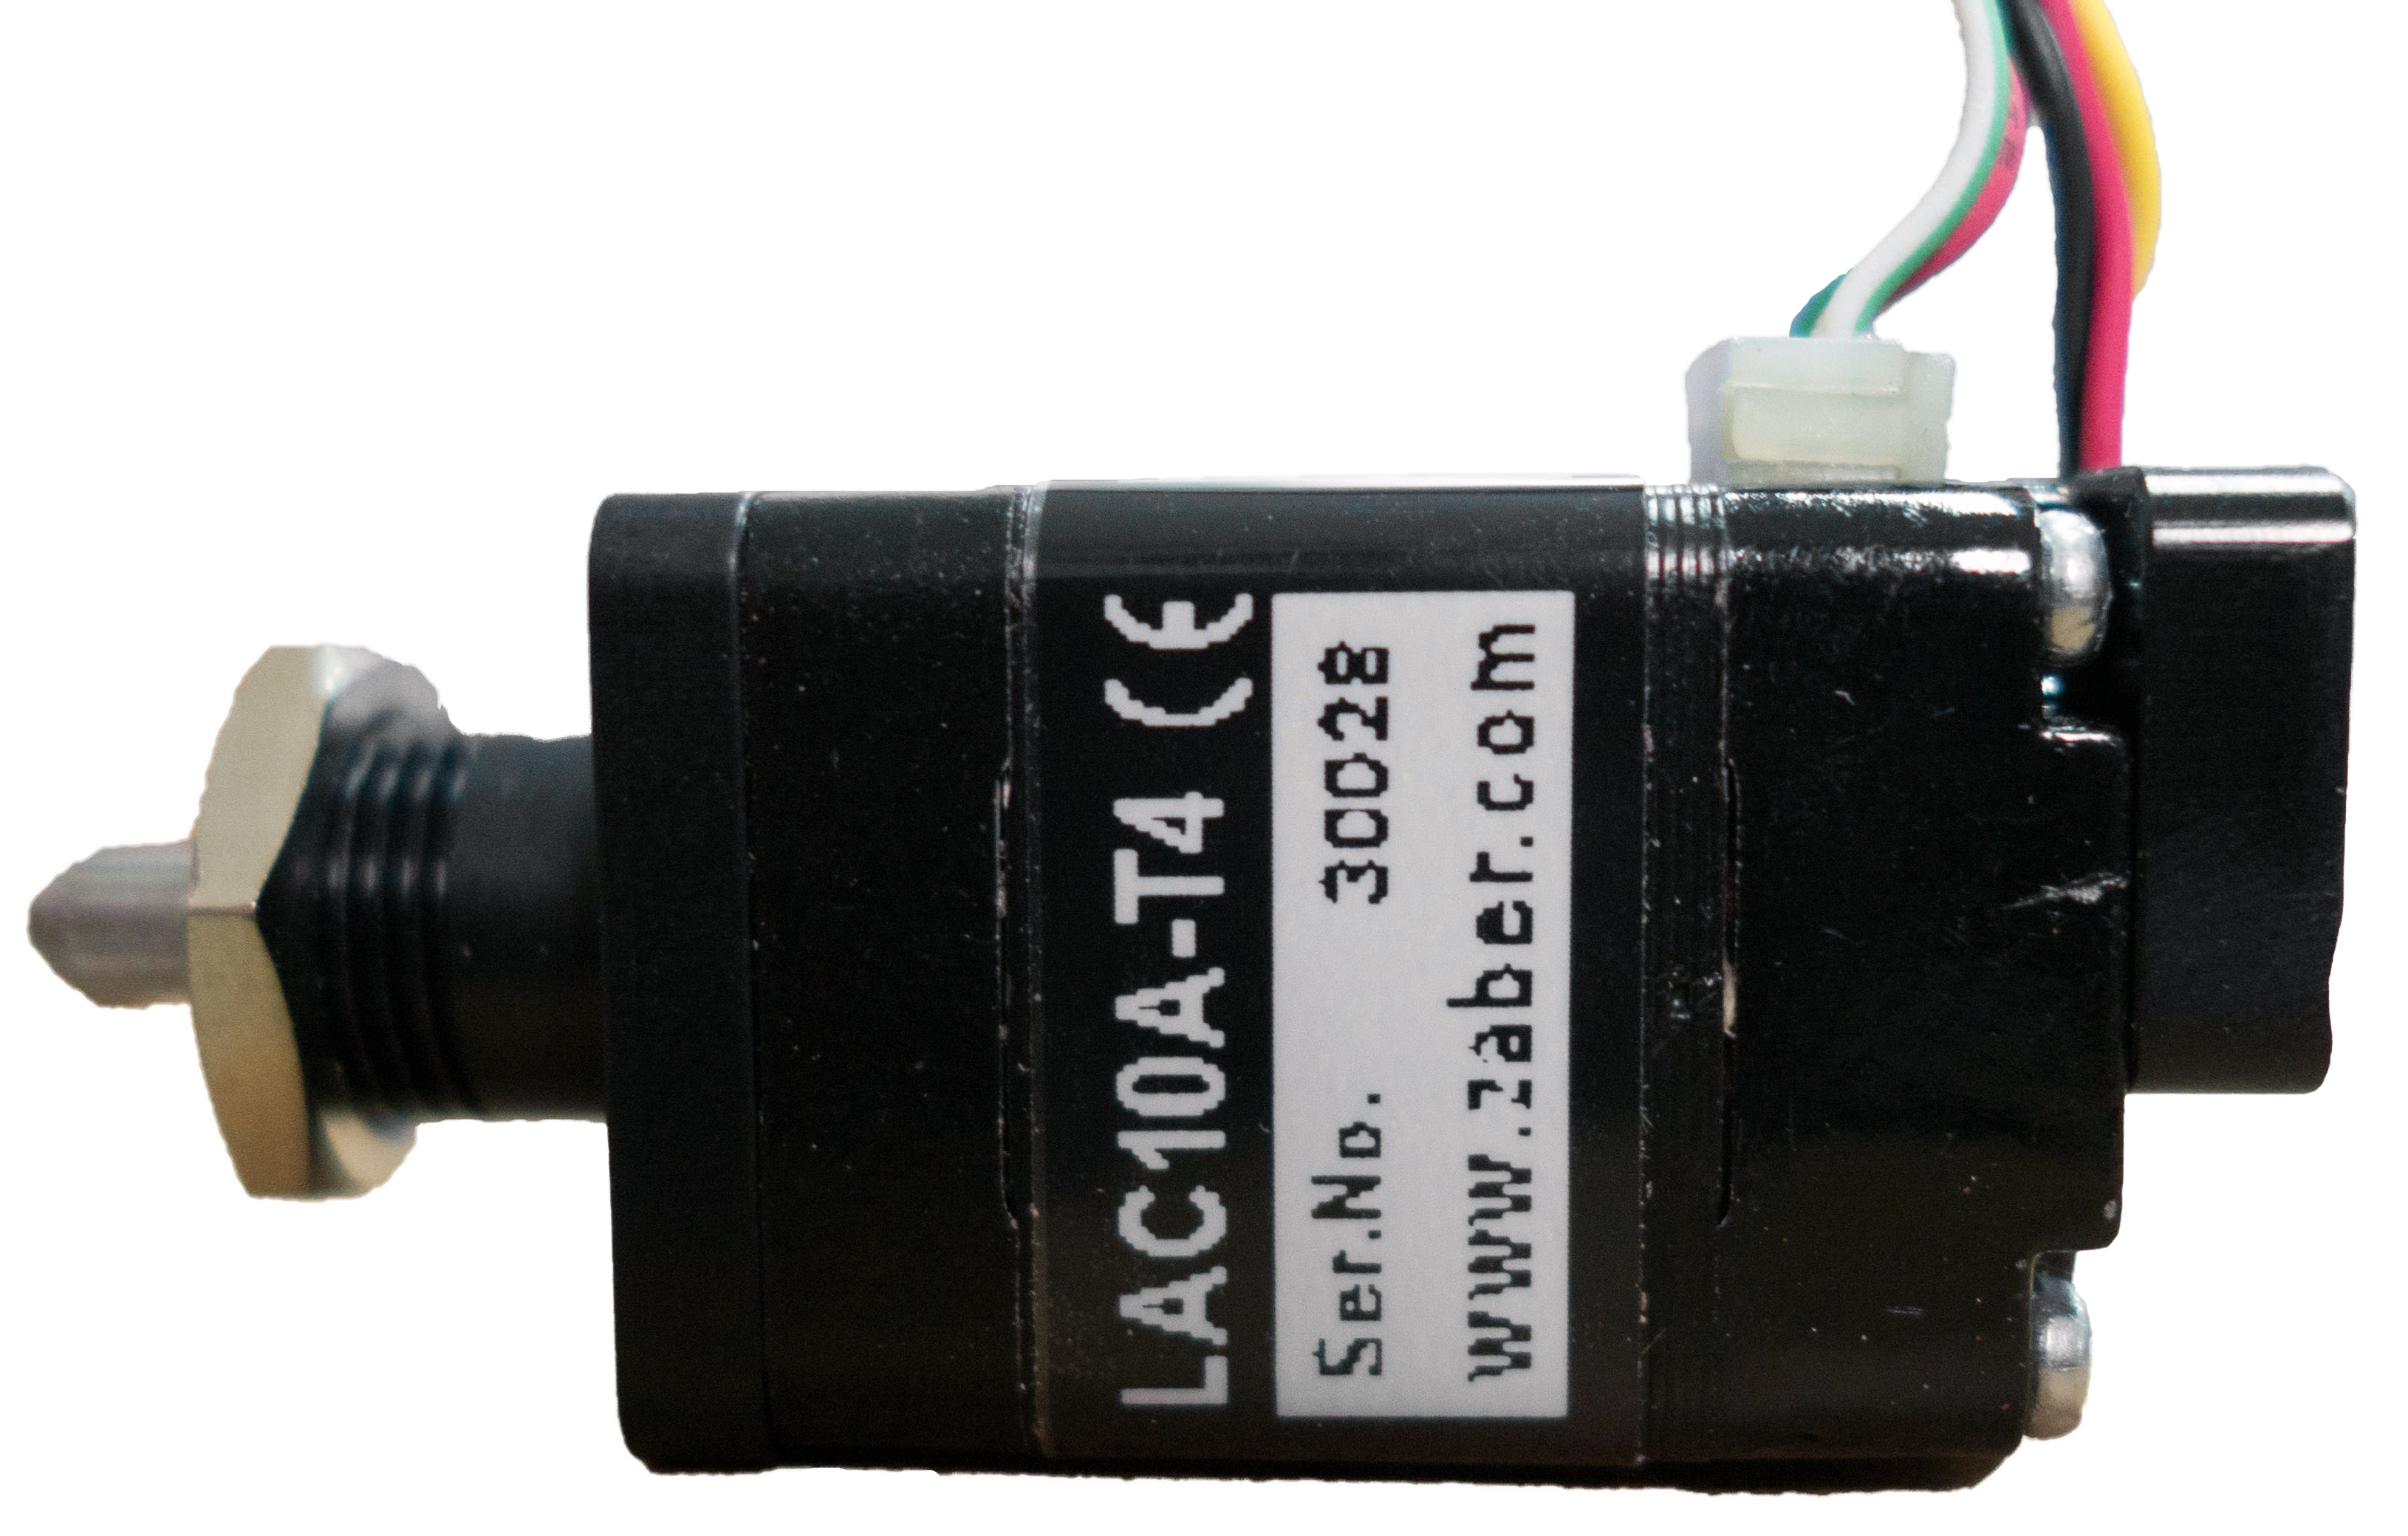
\includegraphics[width=0.618\linewidth]{rig/probe__feeding__LAC10A.png}
\caption{LAC10A-T4精密电动推杆}
\label{fig:rig-probe-feeding-LAC10A}
\end{figure}

\begin{figure}[tbh]
\centering
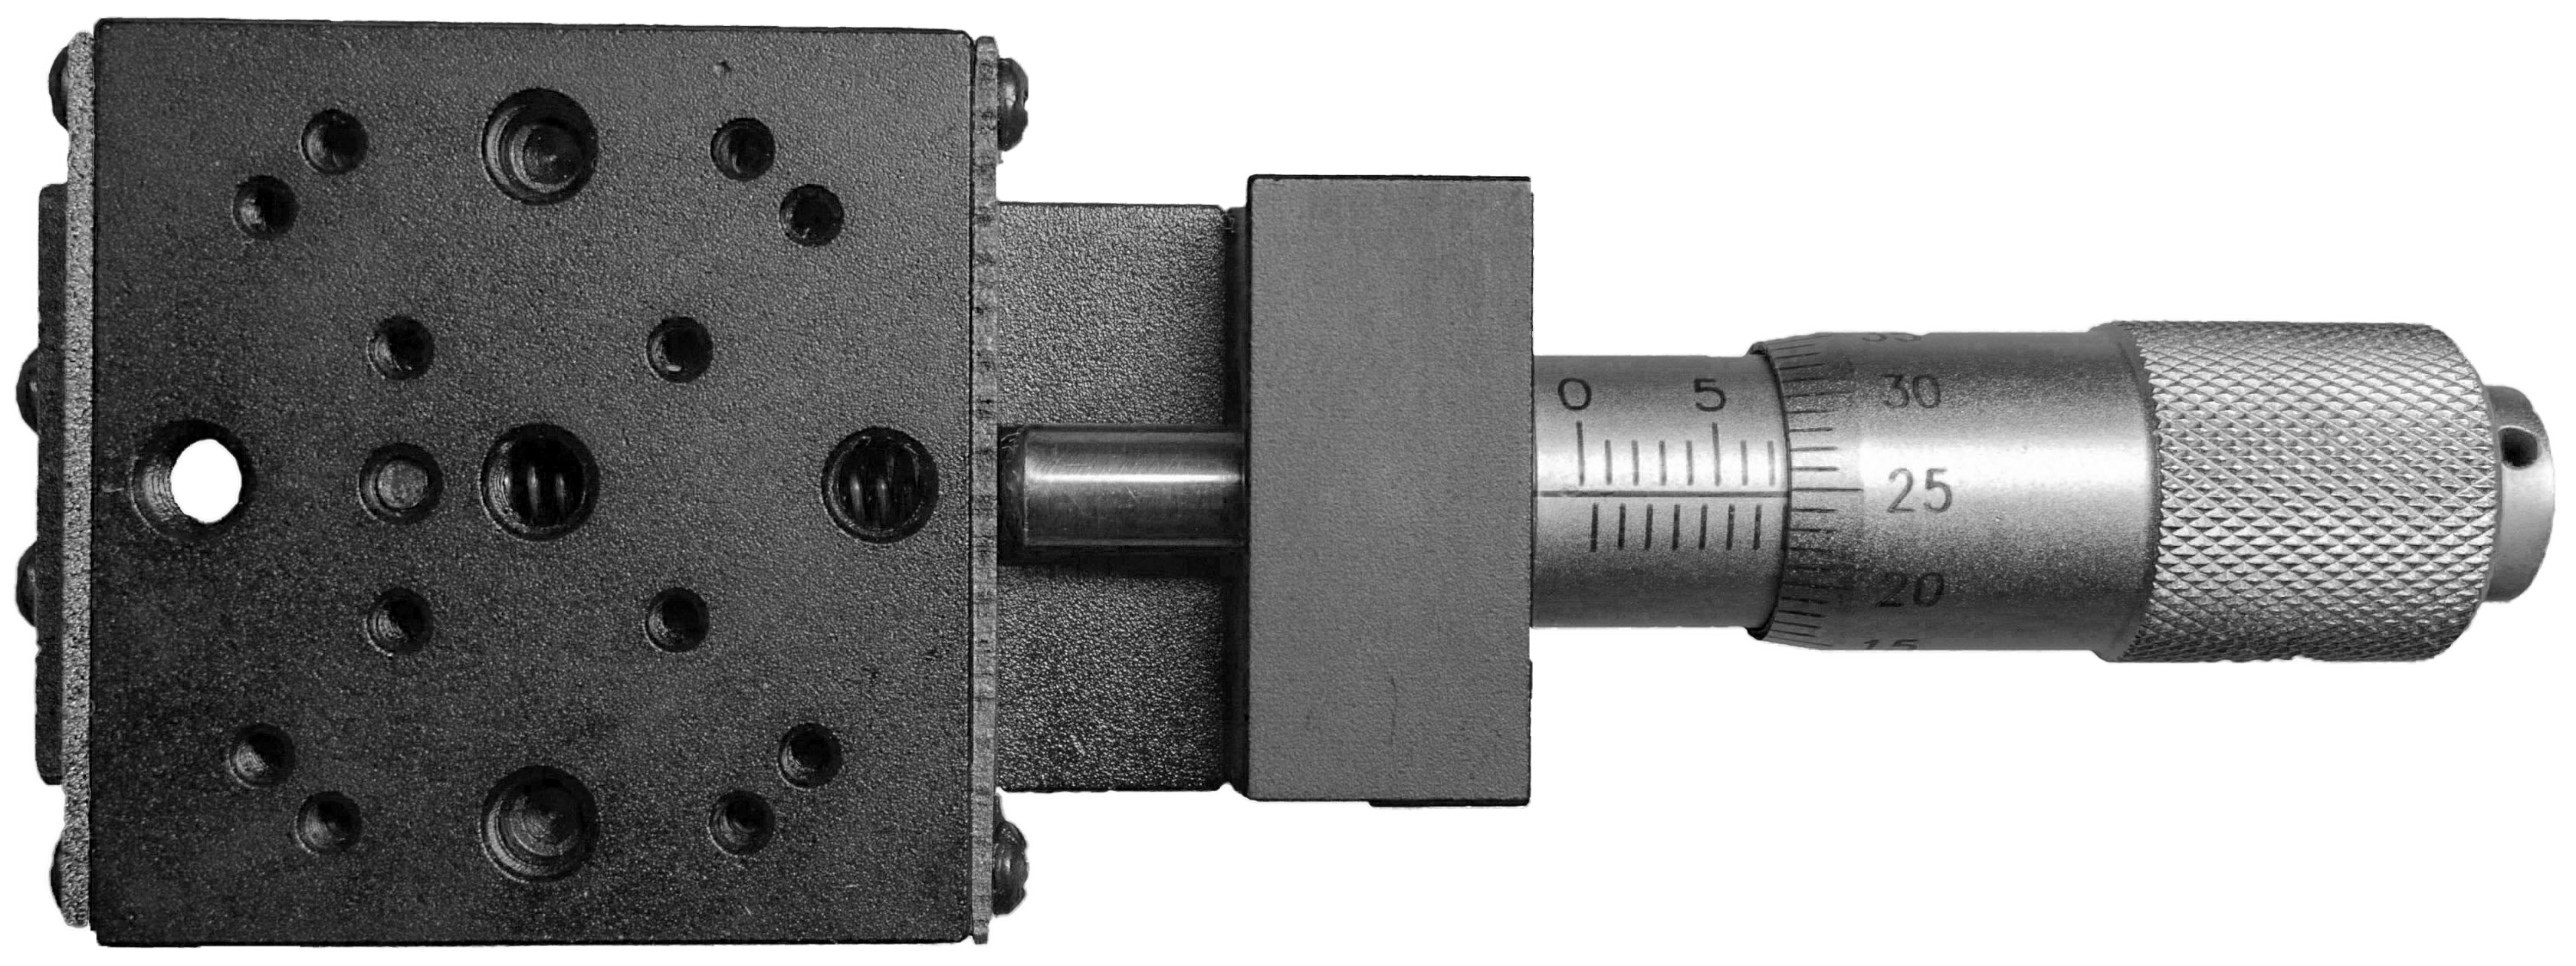
\includegraphics[width=0.618\linewidth]{rig/probe__feeding__JYPY.png}
\caption{JYPY-02213精密手动滑移台}
\label{fig:rig-probe-feeding-JYPY}
\end{figure}



\clearpage



\section{背吹控制系统设计}\label{sec:rig-pressure}

背吹平衡法需要控制静电卡盘背吹入口压强缓慢、平稳上升,并实时测量、记录该压强数值。如能同时测出进入背吹通道的流量,则可为之后的仿真分析提供更多数据参考。整个系统可分为供压与传感两部分,共同的关键参数为压强与流量。按照待测静电卡盘的参数($d = \SI{296}{\mm}$,$F \leq \SI{200}{\N}$)估算背吹入口压强最大值为\SI{5}{\kPa}\footnotemark{}。由于之前尚未有在大气环境下针对同尺寸的静电卡盘的背吹试验或仿真,流量范围未知,只能通过实测获得。本节将分别讨论供压、传感两部分的设计、工作原理与选型。
%then what is \ref{sec:principle-prob-flow-cfd-result}
%apparently it's invalid, but why?

\footnotetext{由于检测平台工作于大气环境下,所有涉及到的压强如无特殊说明均为表压(即相对于大气压强)。}


\subsection{供压方案分析}\label{sec:rig-pressure-supply}

普通气压控制元件(如减压过滤阀等)是为气动机械(如气缸、气爪、气动回转台等)设计的,输出压强下限一般为\SI{0.1}{\MPa}级,超过上文估算的压强范围,因此需使用专用设备实现压强的精确控制。本节依次围绕集成电子压强控制单元、反馈控制微型气泵、以及精密机械式减压阀三个核心组件,提出对应的供压方案。由于影响供压系统性能因素较多,本节仅针对各方案做定性分析,需经实际搭建、测试验证方案可行性与性能。
%TODO:xref pressure impl

\subsubsection{集成电子压强控制单元}\label{sec:rig-pressure-supply-integrated}

这类产品集成了压强控制所需的所有电、气元件,接受一个电信号输入作为压强设定点,控制出口压强等于该设定点。其中,部分产品包括完整的显示、操作单元、通信接口等,如WIKA CPC2000/CPC6000压强控制器等(图~\ref{fig:rig-pressure-supply-cpc6000});部分产品只有简单的指示器,设定点为模拟信号(如$\SIrange{4}{20}{\mA}$信号),如TESCOM ER3000/ER5000系列、SMC ITV00x0系列电子比例阀等。完整的压强控制器较为昂贵,但精度较高,量程可选余地较大;电子比例阀成本较低,但其量程一般仍为气动机械级,而其中较小量程型号允许的流量较低(如SMC ITV0010型,最低输出压强\SI{1}{\kPa},最大流量仅\SI{3.5}{\L\per\minute})。由于这类产品内部集成度较高,组成复杂,且订货周期较长,只能先通过数据手册标称值推测其性能,选取其中参数与供压系统要求匹配较好的产品订购,等待实际搭建验证。
%TODO:xref impl (ITV0010 epic fail, mention PQ already ordered)

\begin{figure}[tbh]
\centering
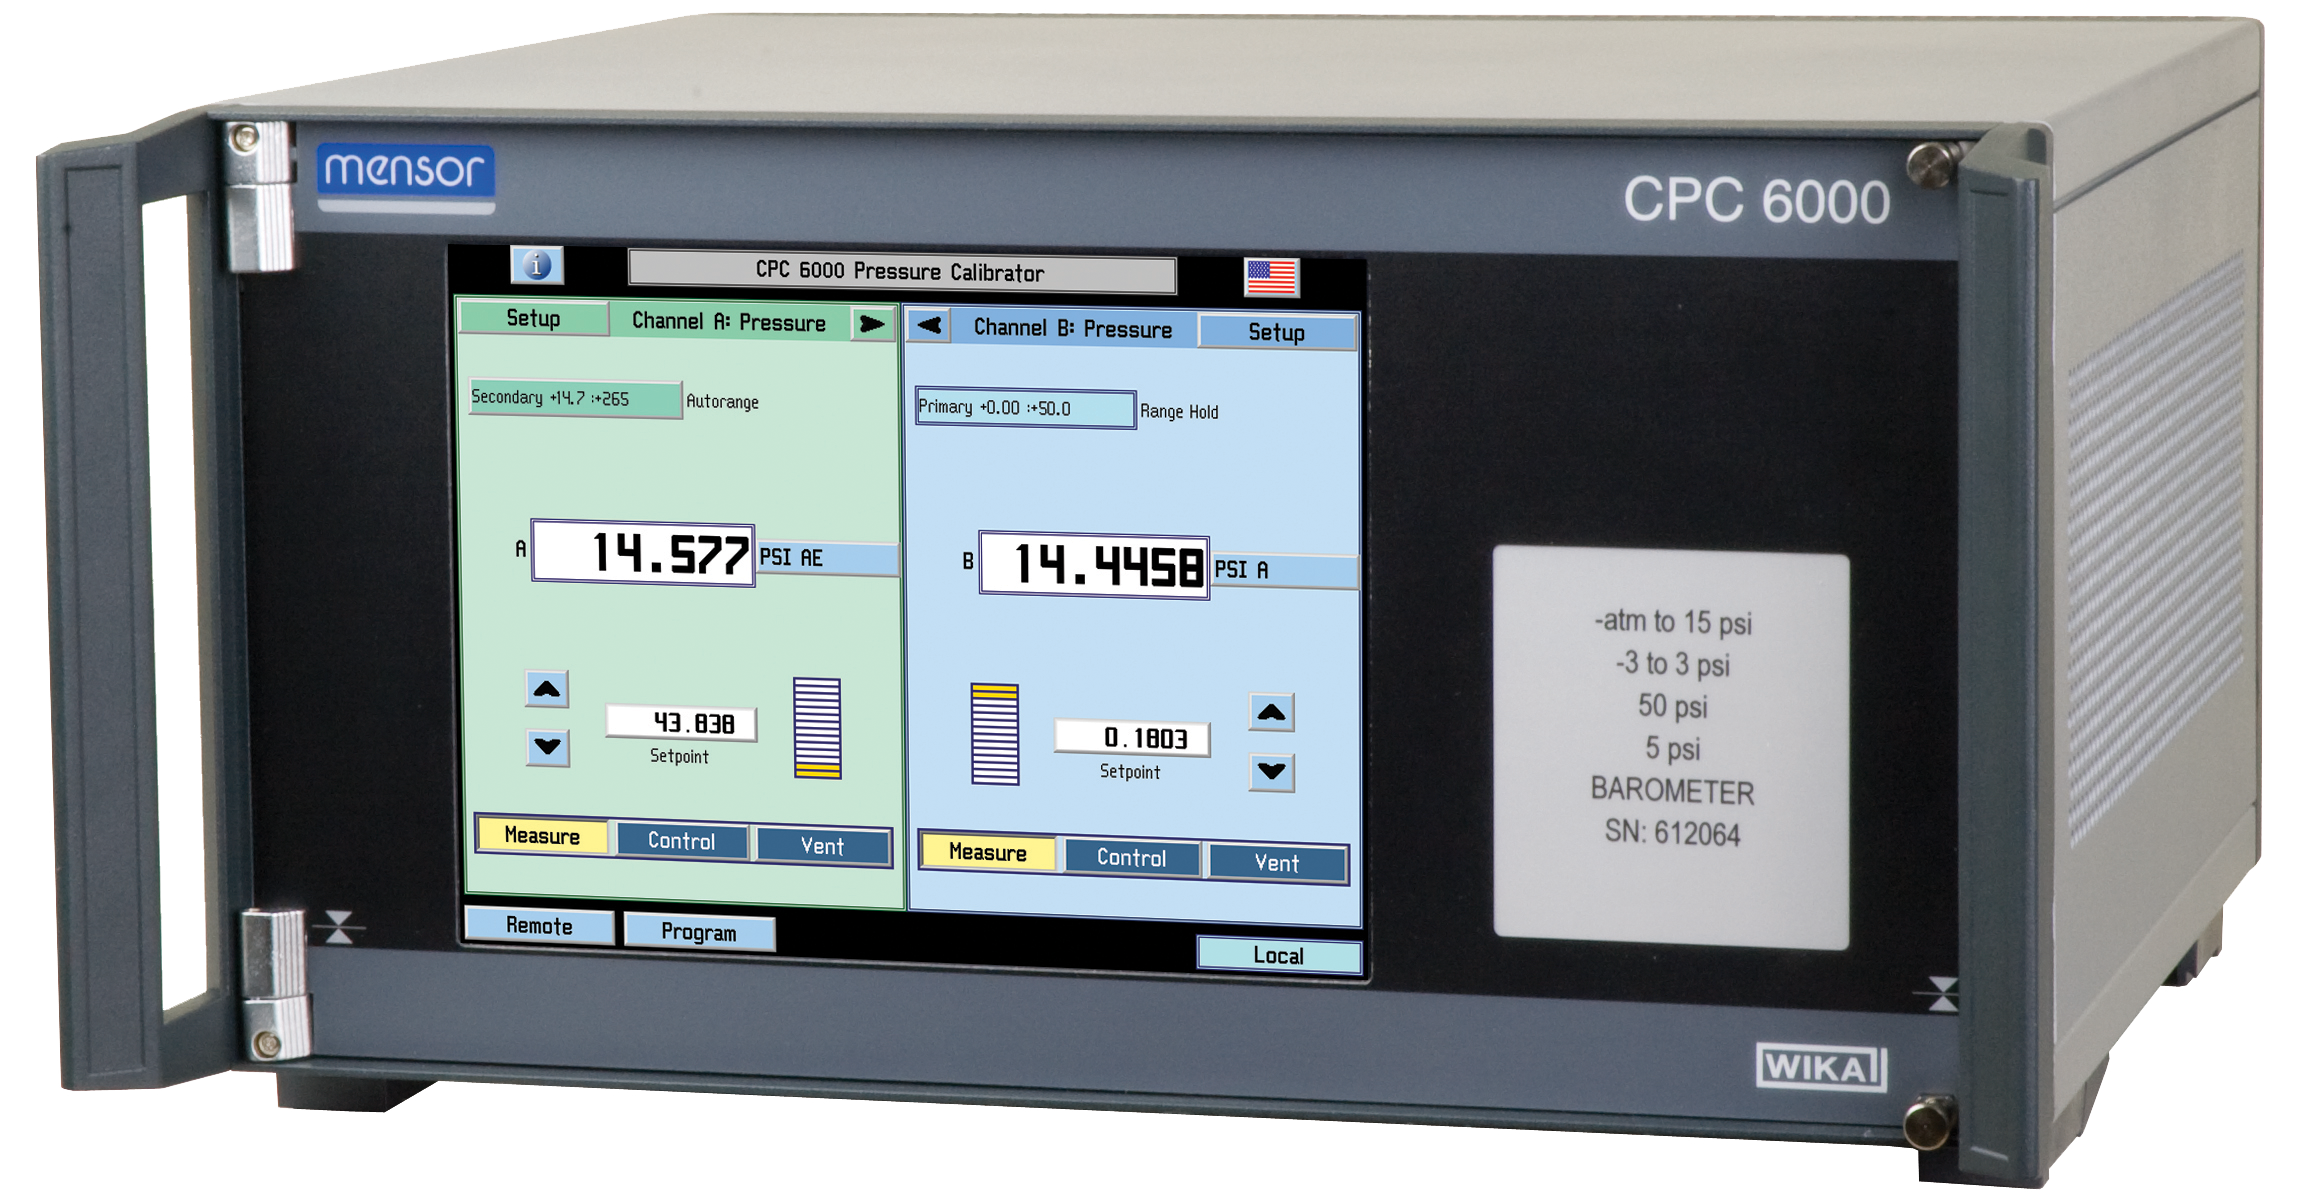
\includegraphics[width=0.75\linewidth]{rig/pressure__supply__cpc6000.png}
\caption{WIKA CPC6000压强控制器}
\label{fig:rig-pressure-supply-cpc6000}
\end{figure}

\subsubsection{反馈控制微型气泵}\label{sec:rig-pressure-supply-pump}

参考图~\ref{fig:rig-pressure-supply-cpc2000-sch},可用独立元件设计类似的压强控制系统,如图~\ref{fig:rig-pressure-supply-pump-sch}:使用直流电机驱动的微型气泵作为压力源,压强变送器提供反馈信号,闭环PI控制气泵输出功率。为减小气泵固有的压强波动,可采取如下措施:

\begin{enumerate}
  \item 在泵与背吹通道入口间增设双端气瓶,通过增加惯性环节的方式降低压强波动;
  \item 在背吹通道入口处加设一节流阀通向大气,避免电机反复启停造成的压强波动;
\end{enumerate}

由于本方案相当于从基础组件开始开发一个完整的闭环控制机电产品,其设计与实现工作量极大,超过本文范畴,不再讨论,仅作为备用方案供参考。

\begin{figure}[tbh]
\centering
\includegraphics[width=1\linewidth]{rig/pressure__supply__cpc2000__sch.png}
\caption{CPC2000工作原理示意}
\label{fig:rig-pressure-supply-cpc2000-sch}
\end{figure}

\begin{figure}[tbhp]
\centering
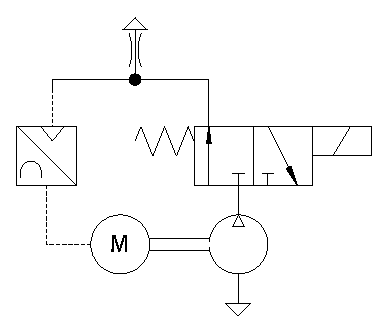
\includegraphics[width=0.5\linewidth]{rig/pressure__supply__pump__sch}
\caption{反馈控制微型气泵示意}
\label{fig:rig-pressure-supply-pump-sch}
\end{figure}

\subsubsection{精密机械式减压阀}\label{sec:rig-pressure-supply-reg}

机械式减压阀的基本原理是:入口与出口间有一开度可调的小孔,其开度由出口压强通过膜片负反馈控制,从而维持出口压强恒定。根据其具体结构不同,部分机械式减压阀在小孔开度接近0时,出口压强可低于其标称最低输出压强,但不能起到稳压作用(即出口压强与流量相关)。如SMC IR1000型精密减压阀(图~\ref{fig:rig-pressure-supply-ir1000}),标称调压范围$\SIrange{5}{200}{\kPa}$,标称灵敏度\SI{0.4}{\kPa}。该产品调压范围可满足\ref{sec:rig-pressure-supply-integrated}节中提到的电子比例阀的入口压强范围要求,因此可作为其前置减压阀使用。同时,虽然其标称最低输出压强大于供压系统最大输出压强,但考虑其工作原理(具有静态放气通路)允许其出口压强低于标称最低输出压强,可以尝试将其出口直接连接背吹入口,用于提供$\SIrange{0}{5}{\kPa}$范围内的缓慢变化的压强。
%TODO:xref impl (manual IR1000 works)

\begin{figure}[tbhp]
\centering
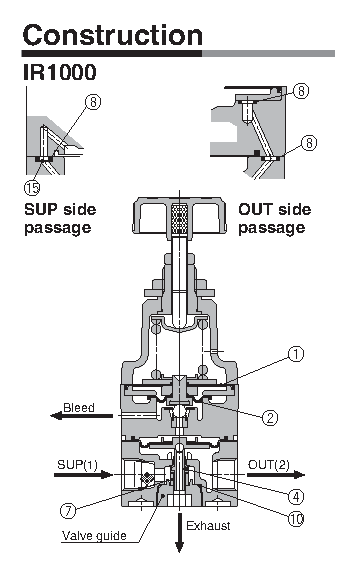
\includegraphics[height=0.55\textheight]{rig/pressure__supply__IR1000}
\caption{IR1000简化剖视}
\label{fig:rig-pressure-supply-ir1000}
\end{figure}


\subsection{传感部分选型}\label{sec:rig-pressure-sensor}

无论供压部分采用何种方案,均不影响压强传感器的选型。完整的选型表见附录B。
%TODO:xref appendix (pressure mashup)
最终选定Honeywell STD720精密差压变送器(量程可在$\pm \num{1} \sim \pm \SI{100}{\kPa}$范围内任意配置,基础准确度$0.05\%$,输出$\SIrange{4}{20}{\mA}$模拟信号、HART现场总线协议)。另外配置\SI{16}{\kPa}量程的机械指针式压强计,辅助调试。


\subsection{过压保护措施}\label{sec:rig-pressure-valve}

由\ref{principle-soln-ruby}节\eqref{eq:principle-soln-ruby-force}式知,晶圆脱附后,微力探头受的压缩力随背吹气压升高而升高,若传感器受力突增至超过其安全过载范围,则有对传感器造成不可恢复的损伤的风险。因此在气路中加入两位三通电磁阀:通电时系统接通压力源,背吹通道压强正常;断电时系统通向大气,背吹通道无压强。在检测过程中,时刻监测传感器受力,一旦超过事先设定的警戒线,立即切断气压,从而避免传感器受损。



\clearpage



\section{机械结构设计}\label{sec:rig-model}

根据图~\ref{fig:rig-overall-sch},设计测试平台的机械结构。为了方便加工、搭建,选用标准$\num{30} \times \SI{30}{\mm}$系列开槽铝合金型材及配套标准连接件,与依据待测静电卡盘的外形尺寸设计的连接板共同构成框架结构;其他组件均通过连接件与之相连。框架结构的简化三维模型如图~\ref{fig:rig-model-all-iso}\footnote{型材连接部分零件数较多,因此并未全部在总装配体三维模型中表示出。}。

\begin{figure}[p]
\centering
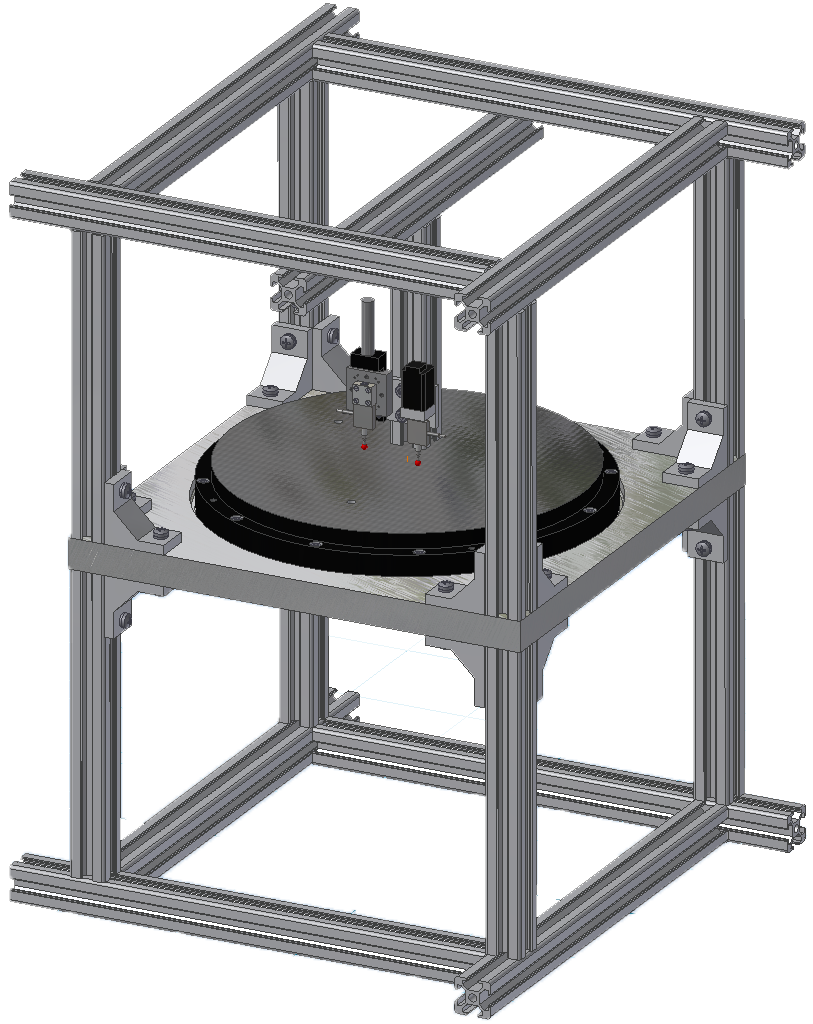
\includegraphics[width=1\textwidth]{rig/model__all__iso.png}
\caption{测试平台装配体三维模型}
\label{fig:rig-model-all-iso}
\end{figure}


\subsection{静电卡盘连接板}\label{sec:rig-model-base}

该连接板位于整个测试平台中心,其尺寸与配合特征主要由静电卡盘决定,并间接决定了整个框架的尺寸。静电卡盘通过螺钉紧固在连接板上,因此连接板需提供相配合的螺纹孔与承载面。如图~\ref{fig:rig-model-echuck-back}\footnotemark{},静电卡盘的底部有多个功能特征,除氦气背吹接口需特殊设计外,其他特征(如直流电极接口、顶针孔等)均需裸露在外以正常使用,因此连接板上对应位置开槽。背吹通道入口并未采用常见的螺纹连接方式,而是一$\diameter{}4$光孔,需设计密封接头与之相连。如图~\ref{fig:rig-model-echuck-plug-assy},用三个紧定螺钉使密封接头上表面与卡盘背面紧密配合,通过标准O型圈形成端面密封;其另一端提供M5内螺纹,与标准气动快装接头连接。

由于连接板图纸幅面较大,此处仅展示其等轴测图(图~\ref{fig:rig-model-echuck-base-iso})。

\footnotetext{北方微电子公司内部图纸,仅保留轮廓与功能描述。}

\begin{figure}[p]
\centering
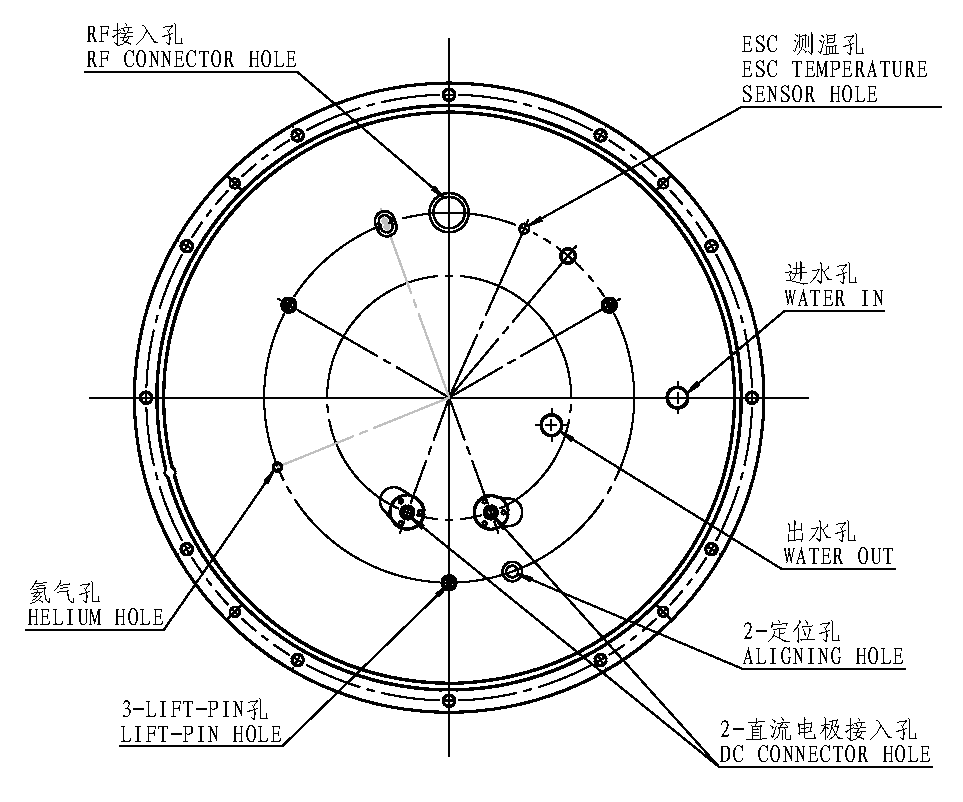
\includegraphics[height=0.45\textheight]{rig/model__echuck__back}
\caption{静电卡盘背面特征工程图}
\label{fig:rig-model-echuck-back}
\end{figure}

\begin{figure}[p]
\centering
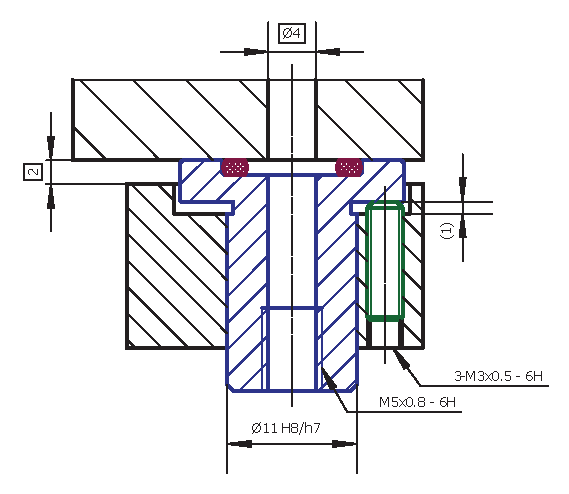
\includegraphics[height=0.45\textheight]{rig/model__echuck__plug__assy2}
\caption{端面密封设计工程图}
\label{fig:rig-model-echuck-plug-assy}
\end{figure}

\begin{figure}[p]
\centering
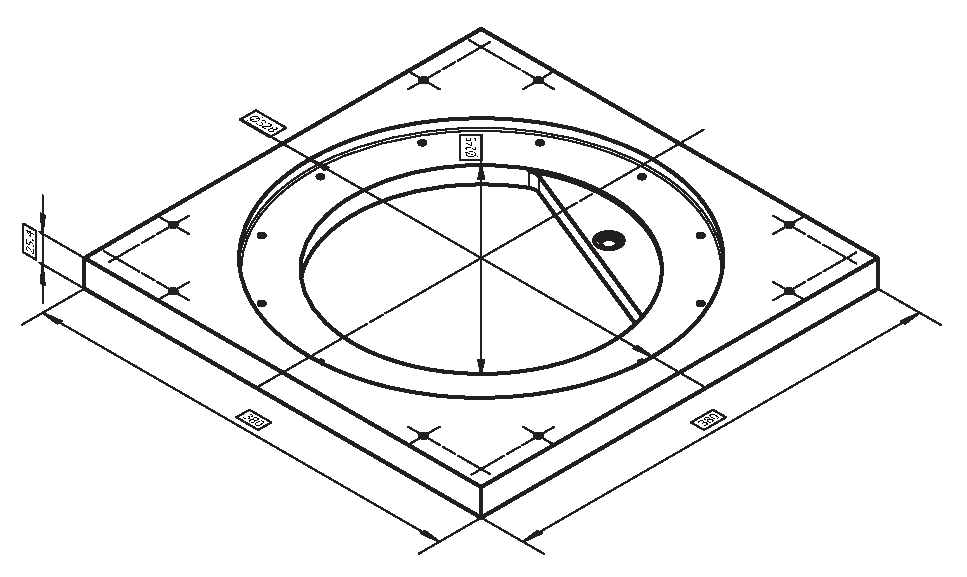
\includegraphics[width=0.618\textwidth]{rig/model__echuck__base__iso}
\caption{静电卡盘连接板等轴测图}
\label{fig:rig-model-echuck-base-iso}
\end{figure}
%TODO:fix the layout!


\subsection{型材框架主体}\label{sec:rig-model-frame}

框架主体设计为三层对称结构:中间一层是静电卡盘连接板,上下两层均为4根型材用铸钢角件和紧定螺钉连接成的正方形结构;层与层之间用4根纵向型材负责承重,在连接板侧使用$\num{50}\times\num{50}\times\SI{30}{\mm}$挤压角件连接(三维模型中已表示出),在正方形框架侧使用$\num{60}\times\num{60}\times\SI{30}{\mm}$角件连接。这种连接方式的主要优点是不依靠型材与角件的摩擦力承受重量,而是靠型材、角件、连接螺栓将载荷传至地面,稳定可靠。


\subsection{微力探头部分}\label{sec:rig-model-probe}

由于红宝石探头的连接螺纹为M2外螺纹,LSB200的连接螺纹为M3内螺纹,设计螺纹转接头如图~\ref{fig:rig-model-probe-connLSBRuby}。由\ref{sec:rig-probe-feeding}节中讨论,需设计微力探头组件位置粗调结构。考虑到LAC-10A电动推杆的行程为\SI{10}{\mm},采用最简单易行的设计(三维模型中已表示出):在框架结构上部加装可自由调节位置的型材组,由横、竖两根型材构成;横梁用螺栓、大垫圈、T槽螺母连接在框架上层四边形的下面;竖梁使用$\num{60}\times\num{60}\times\SI{30}{\mm}$角件与横梁连接。在此基础上,设计微力探头组件连接板如图~\ref{fig:rig-model-probe-connBridgeProbesMain};连接板与LAC-10A通过图~\ref{fig:rig-model-probe-connBridgeProbesTab}~所示连接块、沉头螺钉相连,与JYPY-02213通过沉头螺钉相连。连接板本身可通过螺栓与T槽螺母可紧固在竖梁任意位置。这样即可手动大范围调节微力探头在空间中的位置。
这一部分整体三维模型如图~\ref{fig:rig-model-probe};其中两组微力探头是为了同时在图中表示探头与LAC-10A和JYPY-02213的连接方式,实际仅选装一组。

%TODO:conn JYPY LSB

\begin{figure}[p]
\centering
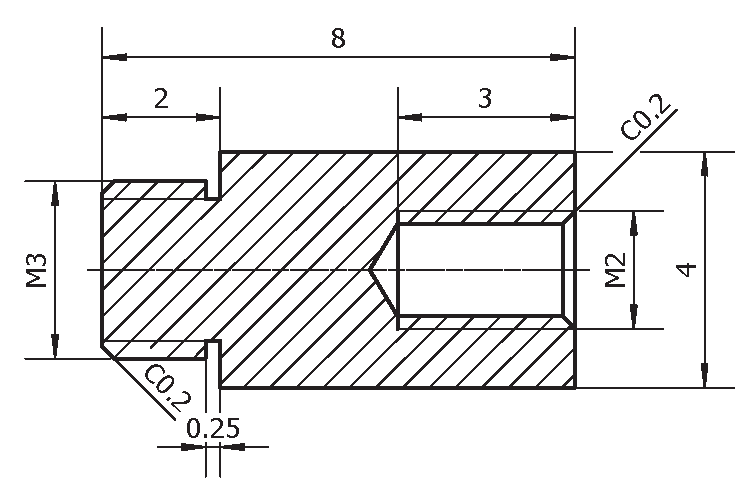
\includegraphics[width=0.618\linewidth]{rig/model__probe__connLSBRuby}
\caption{M2$\to$M3 螺纹转接头零件图}
\label{fig:rig-model-probe-connLSBRuby}
\end{figure}

\begin{figure}[p]
\centering
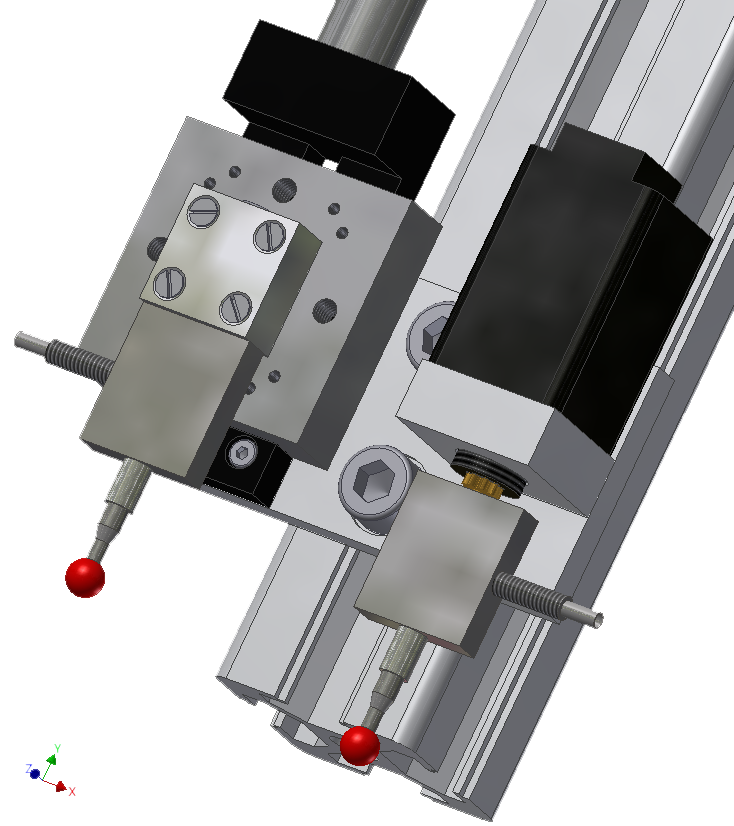
\includegraphics[height=0.35\textheight]{rig/model__probe.png}
\caption{探头组件装配体三维模型}
\label{fig:rig-model-probe}
\end{figure}

\begin{figure}[p]
\centering
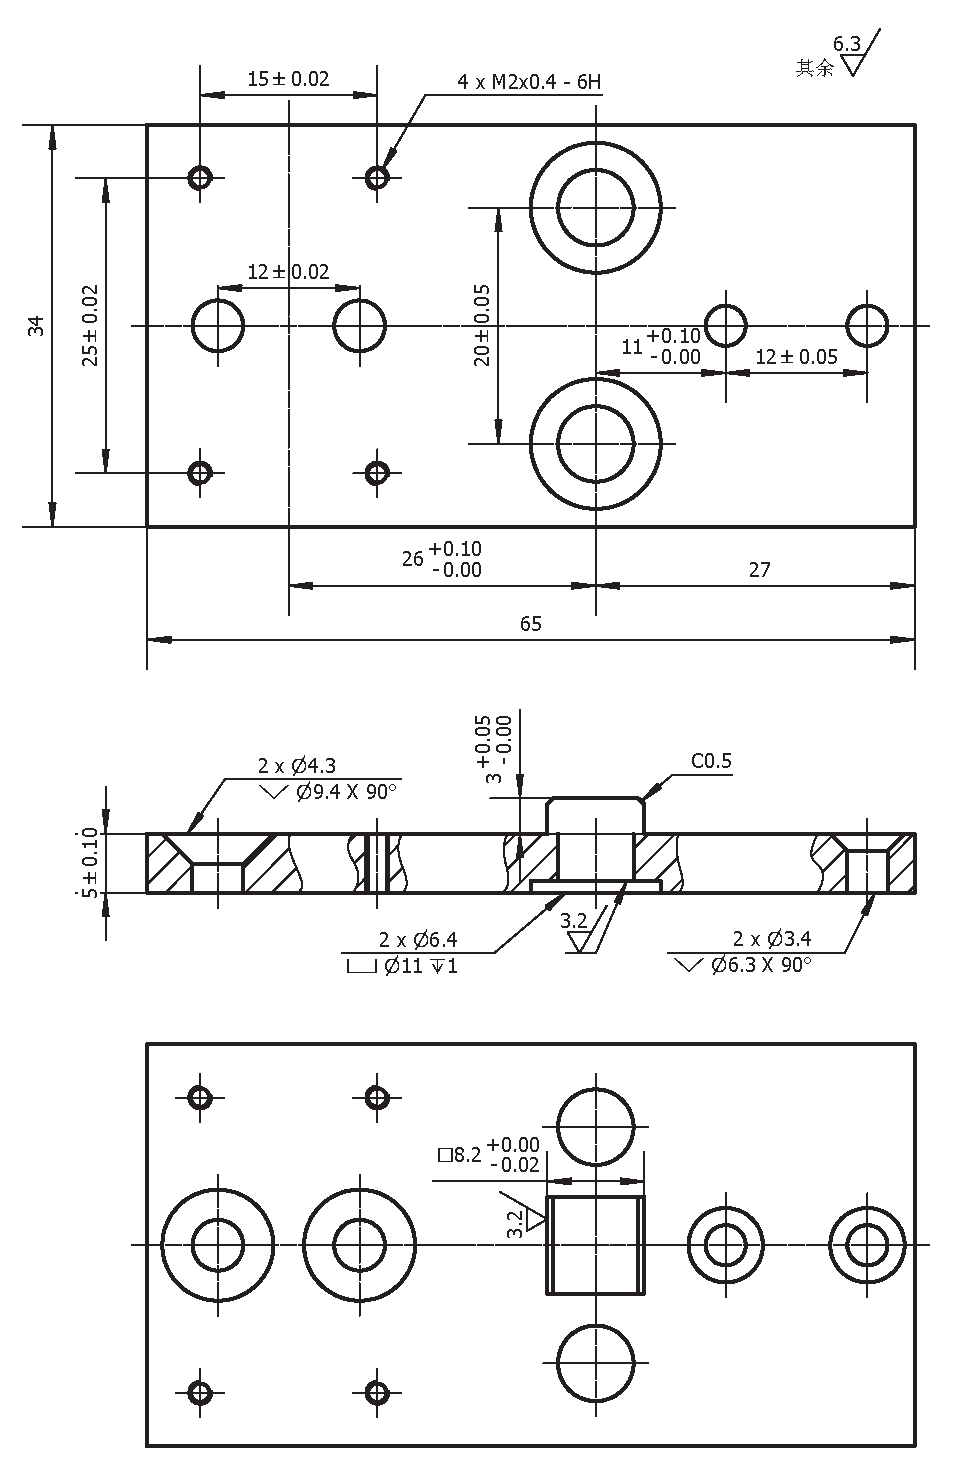
\includegraphics[height=1\textheight]{rig/model__probe__connBridgeProbesMain}
\caption{微力探头组件连接板零件图}
\label{fig:rig-model-probe-connBridgeProbesMain}
\end{figure}

\begin{figure}[p]
\centering
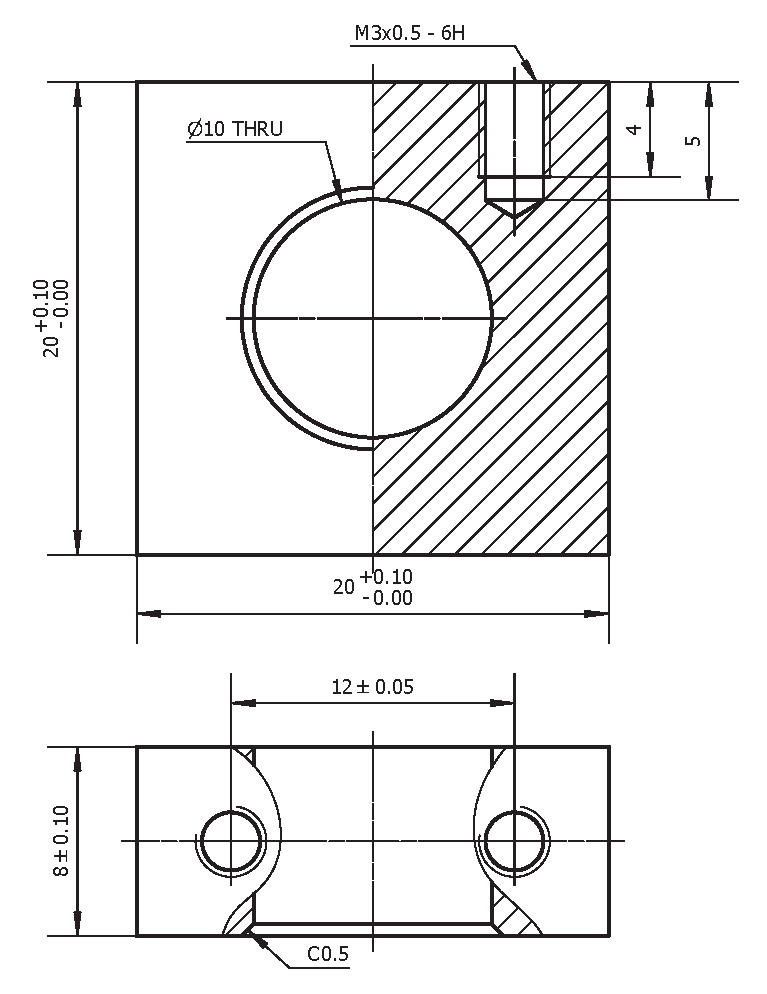
\includegraphics[height=0.48\textheight]{rig/model__probe__connBridgeProbesTab}
\caption{LAC-10A连接块零件图}
\label{fig:rig-model-probe-connBridgeProbesTab}
\end{figure}

\begin{figure}[p]
\centering
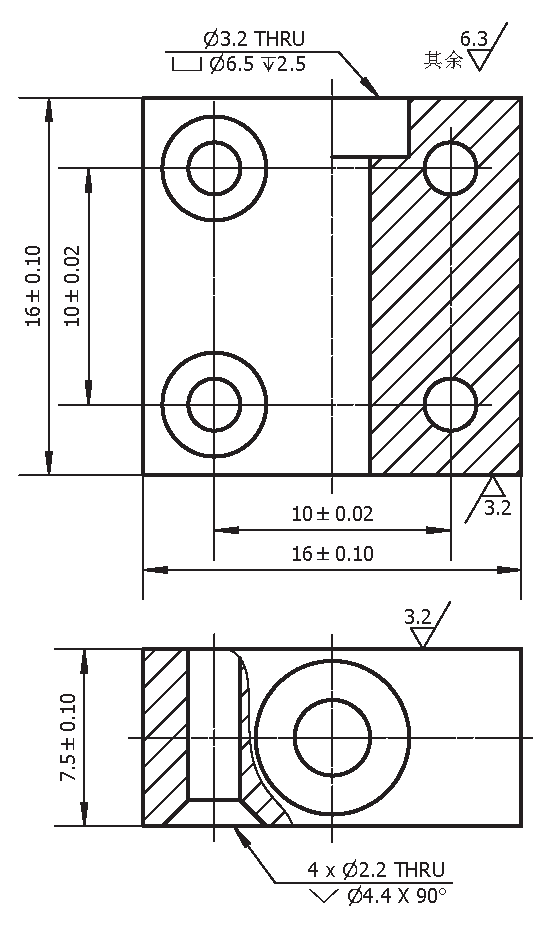
\includegraphics[height=0.42\textheight]{rig/model__probe__connJYPYLSB}
\caption{JYPY-02213连接块零件图}
\label{fig:rig-model-probe-connJYPYLSB}
\end{figure}





\clearpage



\section{自动控制与数据采集系统设计}\label{sec:rig-ctrl}

由于检测平台中存在多种输入输出信号类型各异的电子传感/执行模块,且部分控制对实时性要求高,因此以微控制器单元(MCU)为核心设计自动控制与数据采集系统(下文简称“电控系统”);其组成以及各组件间信号流动关系如图~\ref{fig:rig-ctrl-sch}。可将电控系统分为四个层次,自底向上分别为:传感/执行模块、接口电路、MCU、PC。传感/执行模块即检测平台中使用的压强变送器、电子比例阀、微力传感器等元件。这些模块分散在检测平台各处,接受的输入/输出信号类型各异,需通过匹配的接口电路进行信号处理、转换、隔离等,统一为3.3V电压的数字(包括总线)与模拟信号,再连接到MCU上。本节首先重点针对各传感/执行模块,设计匹配其特性、满足检测平台使用需要的接口电路;然后根据接口电路特点与检测需求,讨论MCU部分的软硬件设计。PC部分主要负责MCU和智能仪表(见\ref{sec:rig-ctrl-intf-loop}节)通信,对其发送指令,接受其回传的数据;这些功能均可使用现有软件完成,不在电控系统具体设计范畴,本节不再讨论。

\begin{figure}[h]
\centering
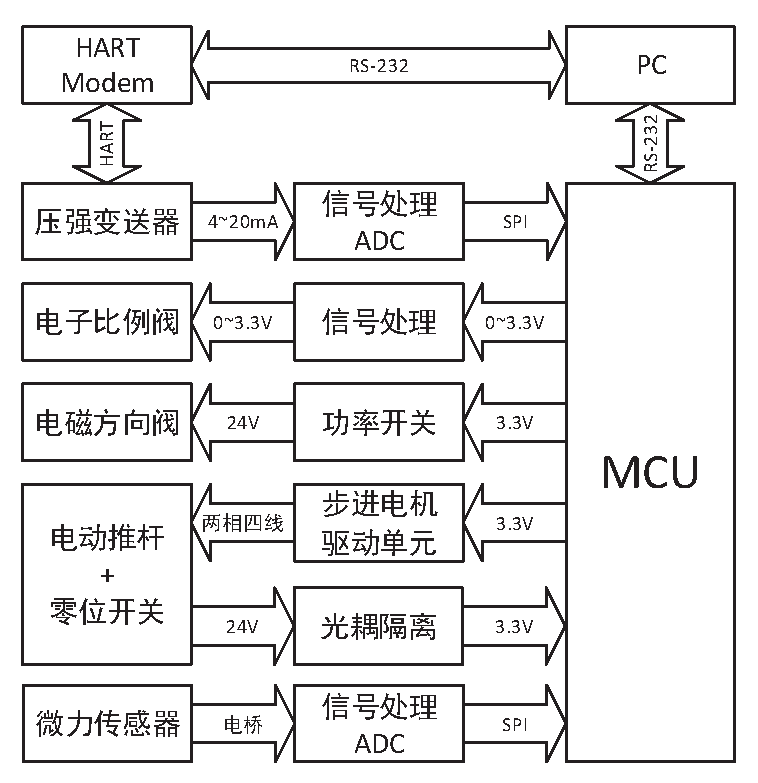
\includegraphics[height=0.5\textheight]{rig/ctrl__sch}
\caption{电控系统组成}
\label{fig:rig-ctrl-sch}
\end{figure}



\subsection{压强变送器接口}\label{sec:rig-ctrl-intf-loop}

\ref{sec:rig-pressure-sensor}节选择的Honeywell STD720精密差压变送器属于Honeywell SmartLine智能数字仪表系列,内置数字信号处理器,为单电源+24V供电的2线制\SIrange{4}{20}{\mA}电流环变送器设备,并支持HART现场总线协议。虽然可以通过HART协议直接从仪表读取压强数值,由于HART传输速率非常低,一个完整的请求 -- 应答过程可耗时\SI{0.25}{\s}以上,与变送器本身的\SI{50}{\Hz}采样率严重不匹配,因此HART协议仅供仪表配置与标定使用,通过独立的HART Modem与PC连接,并使用Honeywell官方提供的软件对其进行配置,而压强的实时数值从\SIrange{4}{20}{\mA}电流环获取。

接口电路总体构成如图~\ref{fig:rig-ctrl-intf-loop-sch-root}:将电流信号转换为电压信号后,接入ADC转换为数字量,由MCU通过SPI串行总线读取。模拟前端(信号转换与处理)部分如图~\ref{fig:rig-ctrl-intf-loop-sch-sample}:稳压滤波过的+24V电压接入变送器正极接线柱(+)为其供电,变送器负极接线柱(-)输出的\SIrange{4}{20}{\mA}电流信号经过\SI{240}{\ohm}采样电阻R2得到\SIrange{0.96}{4.8}{\mV}电压信号,经R3、C1一阶滤波,接入ADC模拟输入端。这里R1起双重作用:与C6组成电源滤波器(并非唯一,见\ref{sec:impl-pcb-pressure}中供电部分),使电流环中串联电阻(R1、R2)不低于\SI{250}{\ohm}以满足HART协议物理层要求。ADC选用AD768x系列\footnotemark{},可直接使用对应数据手册中参考电路,具体实现不再赘述。

\footnotetext{ADI公司AD768x系列、TI公司ADS888x系列为针脚、封装均兼容,功能相同,但性能参数各异的SPI接口SAR(连续逼近)型ADC,由于从ADI公司获取了AD7686样片,下文中该ADC统一称为``AD7686''。}

\begin{figure}[tb]
\centering
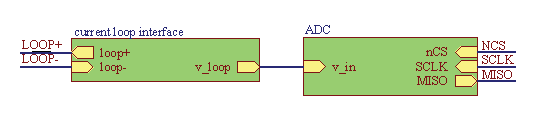
\includegraphics[width=0.8\linewidth]{rig/ctrl__intf__loop__sch__root}
\caption{\SIrange{4}{20}{\mA}电流环接口电路原理图(总体)}
\label{fig:rig-ctrl-intf-loop-sch-root}
\end{figure}

\begin{figure}[tb]
\centering
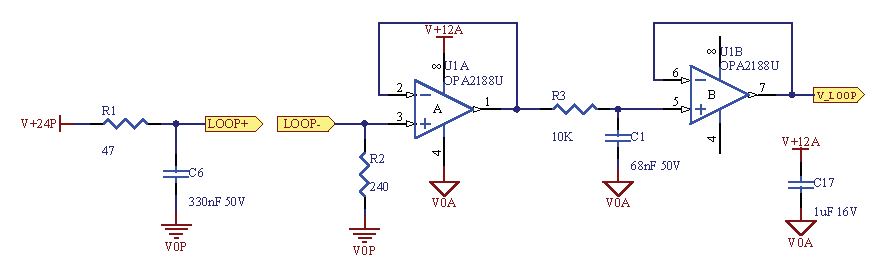
\includegraphics[width=1\linewidth]{rig/ctrl__intf__loop__sch__sample}
\caption{\SIrange{4}{20}{\mA}电流环接口电路原理图(前端)}
\label{fig:rig-ctrl-intf-loop-sch-sample}
\end{figure}

\subsection{电子比例阀接口}\label{sec:rig-ctrl-intf-reg}

\ref{sec:rig-pressure-supply-integrated}节中提到的压力控制器或电子比例阀接受的设定点输入分为两种:模拟电压信号、\SIrange{4}{20}{\mA}模拟电流环信号。模拟电压输入可直接通过单片机内置DAC(输出范围\SIrange{0}{3.3}{\V})经一级放大滤波得到,其原理图与图\ref{fig:rig-ctrl-intf-loop-sch-sample}~中采样电阻之后的部分基本相同,不再赘述。模拟电流输入可用AD420集成电流输出DAC提供,接法如图~\ref{fig:rig-ctrl-intf-ad420}。

\begin{figure}[tbhp]
\centering
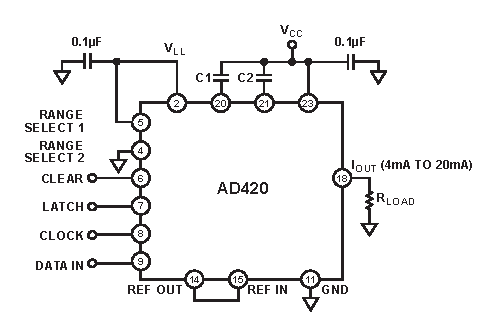
\includegraphics[width=0.618\linewidth]{rig/ctrl__intf__ad420}
\caption{AD420接法原理图}
\label{fig:rig-ctrl-intf-ad420}
\end{figure}

\subsection{电磁方向阀接口}\label{sec:rig-ctrl-intf-relay}

\ref{sec:rig-pressure-valve}节中的电磁方向阀(两位三通)在电路中等效为一直流\SI{24}{\V}继电器,可使用常见的ULN2003集成功率开关驱动,如图~\ref{fig:rig-ctrl-intf-uln2003}。由于ULN2003内置续流二极管,输出端无需任何被动元件;R14为输入端下拉电阻,防止输入悬空时受电磁干扰产生误动作。

\begin{figure}[tbhp]
\centering
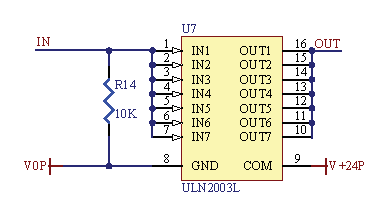
\includegraphics[width=0.618\linewidth]{rig/ctrl__intf__uln2003}
\caption{ULN2003功率开关原理图}
\label{fig:rig-ctrl-intf-uln2003}
\end{figure}

\subsection{电动推杆接口}\label{sec:rig-ctrl-intf-stepper}

\ref{sec:rig-probe-feeding}节中选择的LAC-10A电动推杆使用两相四线混合式步进电机作为驱动力,并使用永磁铁 -- 霍尔开关作为零位传感器。该步进电机的相电阻较高,为\SI{20.4}{\ohm},而额定电流较低,为\SI{0.24}{\A},需要使用与之相匹配的步进电机驱动器。最终选择雷赛DM422C数字式步进电机驱动器,其输出峰值电流可事先以\SI{0.1}{\A}为单位通过串口配置,通过2片MAX490E差分输入输出接口芯片(图~\ref{fig:rig-ctrl-intf-max490e})分别接收MCU发出的脉冲、方向指令信号。

LAC-10A附带的零位传感器使用标准的3线开漏(open drain)输出霍尔开关A1122:平时输出悬空;当在电动推杆即将到达其最短位置时,磁铁靠近霍尔开关,使其动作,输出被下拉至地;由于霍尔开关具有滞回(hysterisis),此时只有电动推杆向伸长方向移动一小段确定的距离后,输出才会恢复悬空状态。由于电机附近存在较强电磁干扰,为避免因此产生误动作,可增加霍尔开关供电电压至\SIrange{12}{24}{\V}\footnotemark{},通过光耦隔离,转换为\SI{3.3}{\V}信号,如图~\ref{fig:rig-ctrl-intf-opto}:U2为普通光耦,R1为光耦输入端串联限流电阻,输出端R2为上拉电阻。零位传感器等效为开关J1,平时J1断开,\bverb|out|为高电平(\SI{3.3}{\V});动作时J1闭合,U2接通,\bverb|out|为低电平(0);该信号即可直接接入MCU。

\footnotetext{A1122数据手册中标称\SI{24}{\V}为最大供给电压,因此实际供给电压应 严格小于\SI{24}{\V}。}

\begin{figure}[p]
\centering
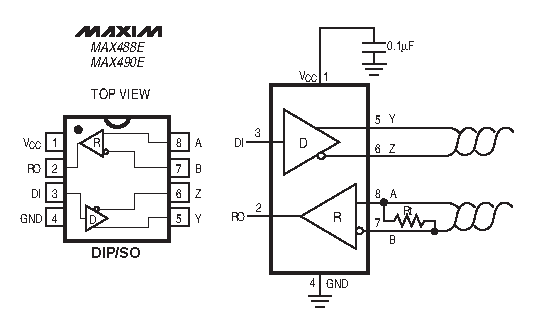
\includegraphics[width=0.7\linewidth]{rig/ctrl__intf__max490e}
\caption{MAX490E差分输入输出原理图}
\label{fig:rig-ctrl-intf-max490e}
\end{figure}

\begin{figure}[p]
\centering
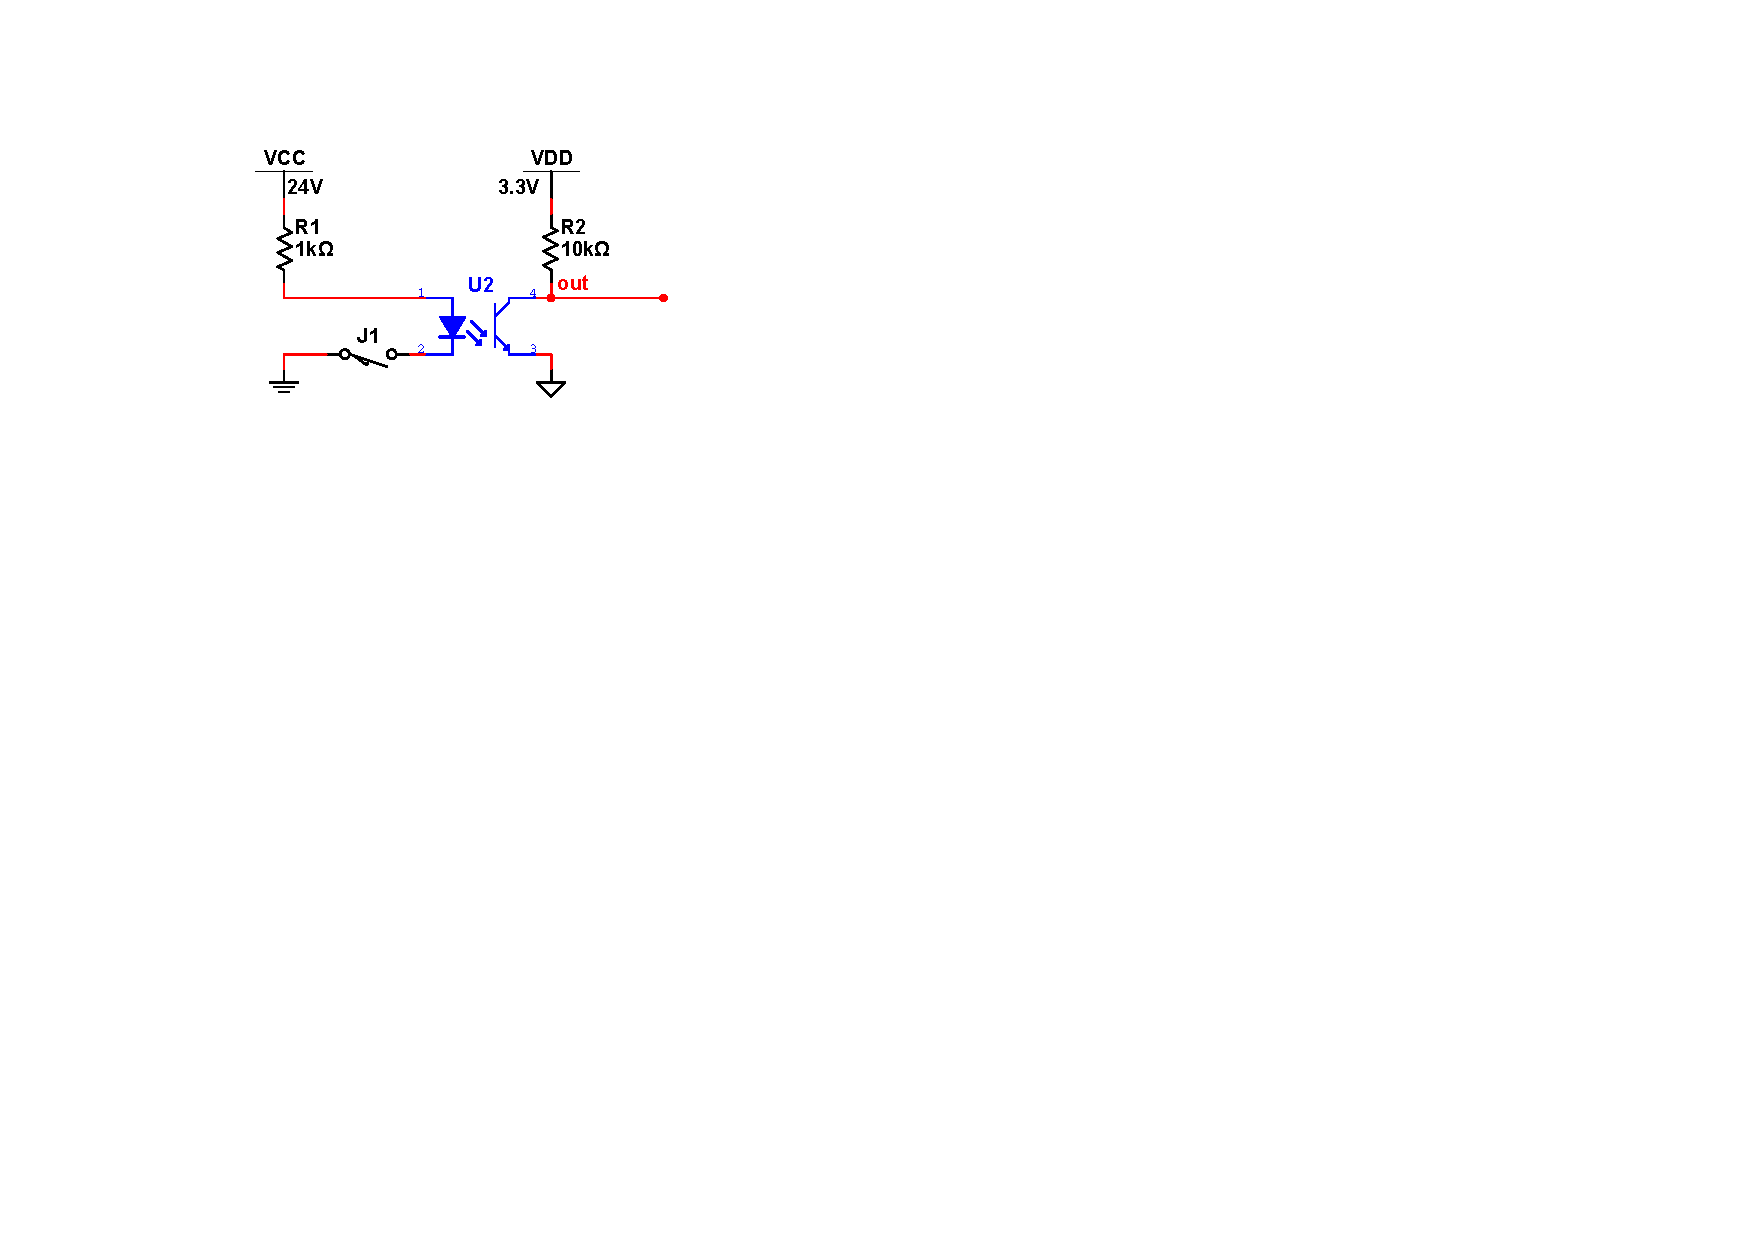
\includegraphics[width=0.5\linewidth]{rig/ctrl__intf__opto}
\caption{LAC-10A零位传感器 -- 光耦接口 -- 原理图}
\label{fig:rig-ctrl-intf-opto}
\end{figure}

\subsection{微力传感器接口}\label{sec:rig-ctrl-intf-strain}

\ref{sec:rig-probe-sensor}节中选择的LSB200应变式微力传感器,其敏感元件为随受力变化而线性变化的电阻应变片,在内部接为电桥,如图~\ref{fig:rig-ctrl-strain-bridge}。电桥式传感器的基本原理如下:在\bverb|E+|、\bverb|E-|(E为excitation的缩写)两端加电压$V_{\mathrm{E}}$后,\bverb|S+|、\bverb|S-|(S为signal的缩写)两端电压为:
\[
V_{\mathrm{S}} = V_{\mathrm{E}} \cdot (\frac{R_2}{R_1 + R_2} - \frac{R_4}{R_3 + R_4})
\]
根据此关系,传感器被设计为满足:
\begin{equation}
\label{eq:rig-ctrl-intf-strain}
\frac{V_{\mathrm{S}}}{V_{\mathrm{E}}} = k (F + F_0)
\end{equation}
其中$F$为传感器受力,$k$为只与应变片本身特性相关的比例系数,$F_0$为传感器的零位偏差。

LSB200主要参数:阻值\SI{1000}{\ohm},标称满量程输出\SI{0.5}{\mV\per\V},最大激励电压\SI{10}{\V}。由于电桥的等效输出电阻低,输出电压最大为\SI{5}{\mV},需将该信号放大后处理。考虑到压强变送器内部采样率仅为\SI{50}{\Hz}(见\ref{sec:rig-ctrl-intf-loop}节),微力传感器无需高采样率;为简化电路,减小可能干扰脱附判断的噪声,选择专门为低速($\leq\SI{1}{\kHz}$)电桥设计的集成了可变增益仪表放大器与24位$\Sigma$--$\Delta$型ADC的AD7730芯片,如图~\ref{fig:rig-ctrl-ad7730-ac}。由于ADC的转换结果由其输入电压与参考电压的比值决定,一般必须使用精确电压基准芯片为ADC提供参考电压,才能得到准确的转换结果;但在本电路中,ADC参考电压与激励电压相同,均为$V_{\mathrm{E}}$,由\eqref{eq:rig-ctrl-intf-strain}式知,参考电压的变化不影响输入电压与参考电压的比值,即转换结果与参考电压具体取值无关,所以无需使用精确电压基准芯片。AD7730的参考电压名义值为\SI{5}{\V},输入电压范围名义值(即放大器增益)可通过SPI接口设定为\SIlist[list-separator={、},list-final-separator={、或}]{\pm 10;\pm 20;\pm 40;\pm 80}{\mV};当$V_{\mathrm{E}} = \SI{5}{\V}$时,$V_{\mathrm{S}}$范围为\SI{\pm 2.5}{\mV},因此设定AD7730的电压范围为\SI{\pm 10}{\mV}。

\begin{figure}[p]
\centering
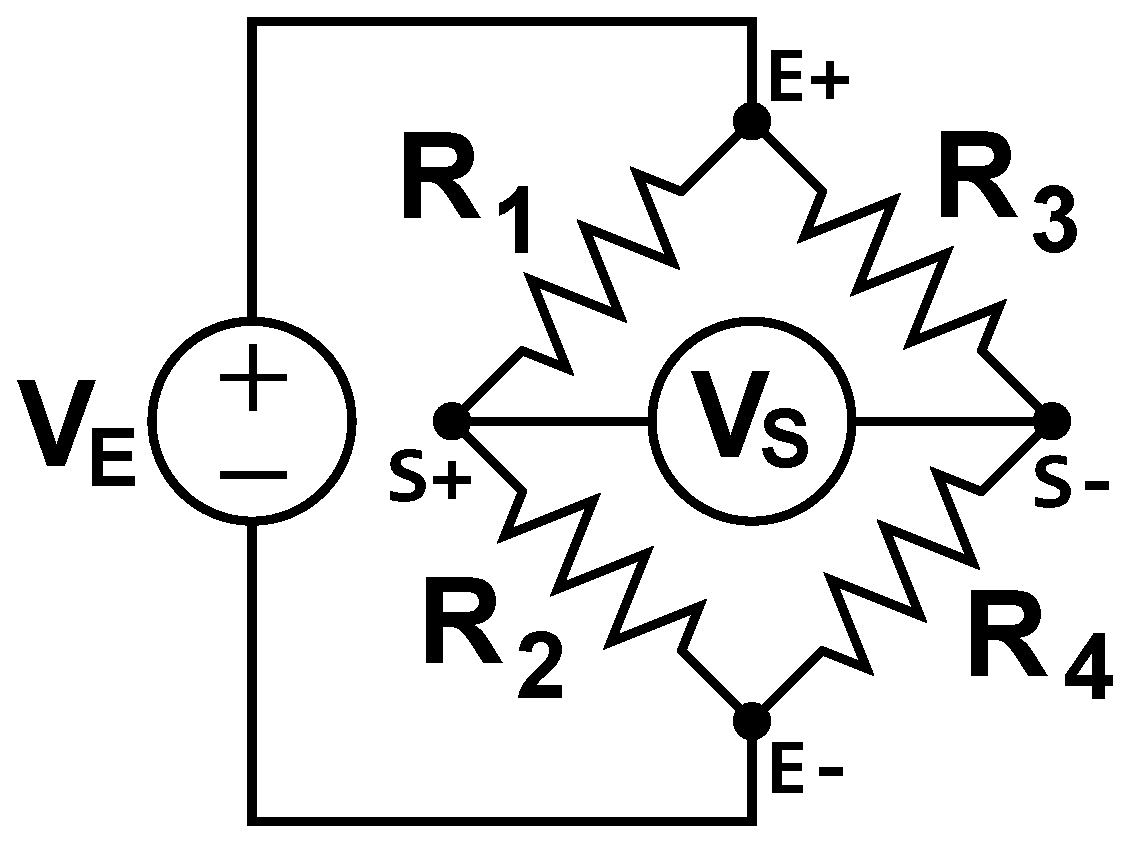
\includegraphics[width=0.4\linewidth]{rig/ctrl__intf__strain__bridge}
\caption{应变片电桥等效电路}
\label{fig:rig-ctrl-strain-bridge}
\end{figure}

\begin{sidewaysfigure}[p]
\centering
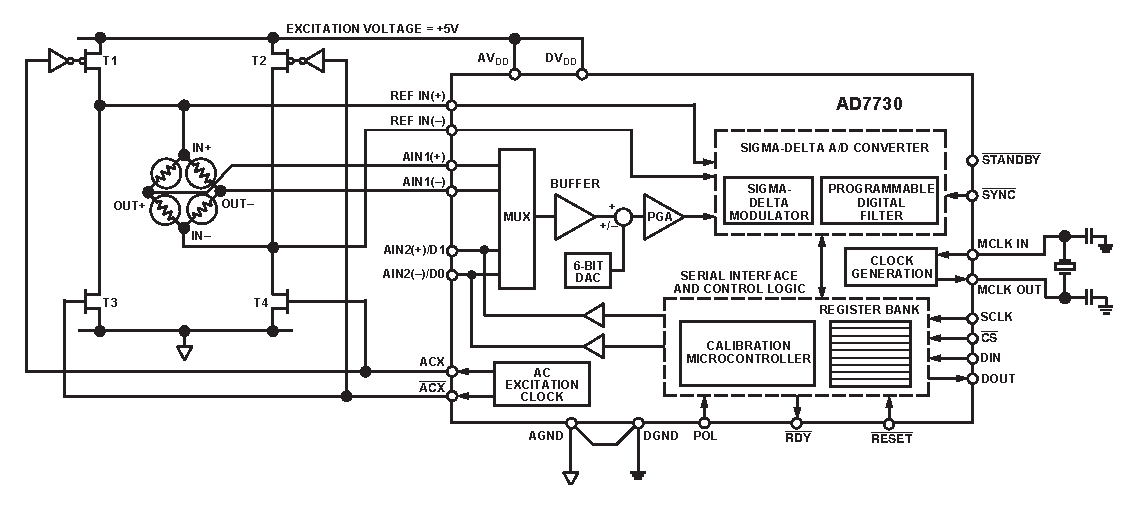
\includegraphics[width=1\linewidth]{rig/ctrl__intf__ad7730__ac}
\caption{AD7730电桥接口 -- 接法示意图}
\label{fig:rig-ctrl-ad7730-ac}
\end{sidewaysfigure}


\clearpage


\subsection{微控制器单元(MCU)}\label{sec:rig-ctrl-mcu}

由于电控系统无占用空间、耗电等特殊需求,选择常用的具有较强处理能力以及丰富外设的STM32F1系列ARM Cortex-M3内核32位MCU,以方便后续开发与扩展。结合图~\ref{fig:rig-ctrl-sch}~以及各接口电路具体设计,规划MCU外设与针脚资源如图~\ref{fig:rig-ctrl-mcu-pinout}:\bverb|SPI1|及附近针脚连接压强采样ADC(AD7686,见\ref{sec:rig-ctrl-intf-loop}节),\bverb|SPI2|及附近针脚连接微力传感器采样ADC(AD7730,见\ref{sec:rig-ctrl-intf-strain}节);定时器\bverb|TIM4|向步进电机驱动器输出脉冲,外部中断\bverb|EXTI14|处理电动推杆零位传感器信号(\ref{sec:rig-ctrl-intf-stepper}节);\bverb|DAC|向电子比例阀接口(\ref{sec:rig-ctrl-intf-reg}节)提供设定点模拟信号;串口\bverb|USART1|与PC交换数据,\bverb|USART2|保留供MCU通过HART主机模块自动配置压强变送器,\bverb|USART3|保留供其他可能加入电控系统的串口外设使用。

\begin{figure}[tbhp]
\centering
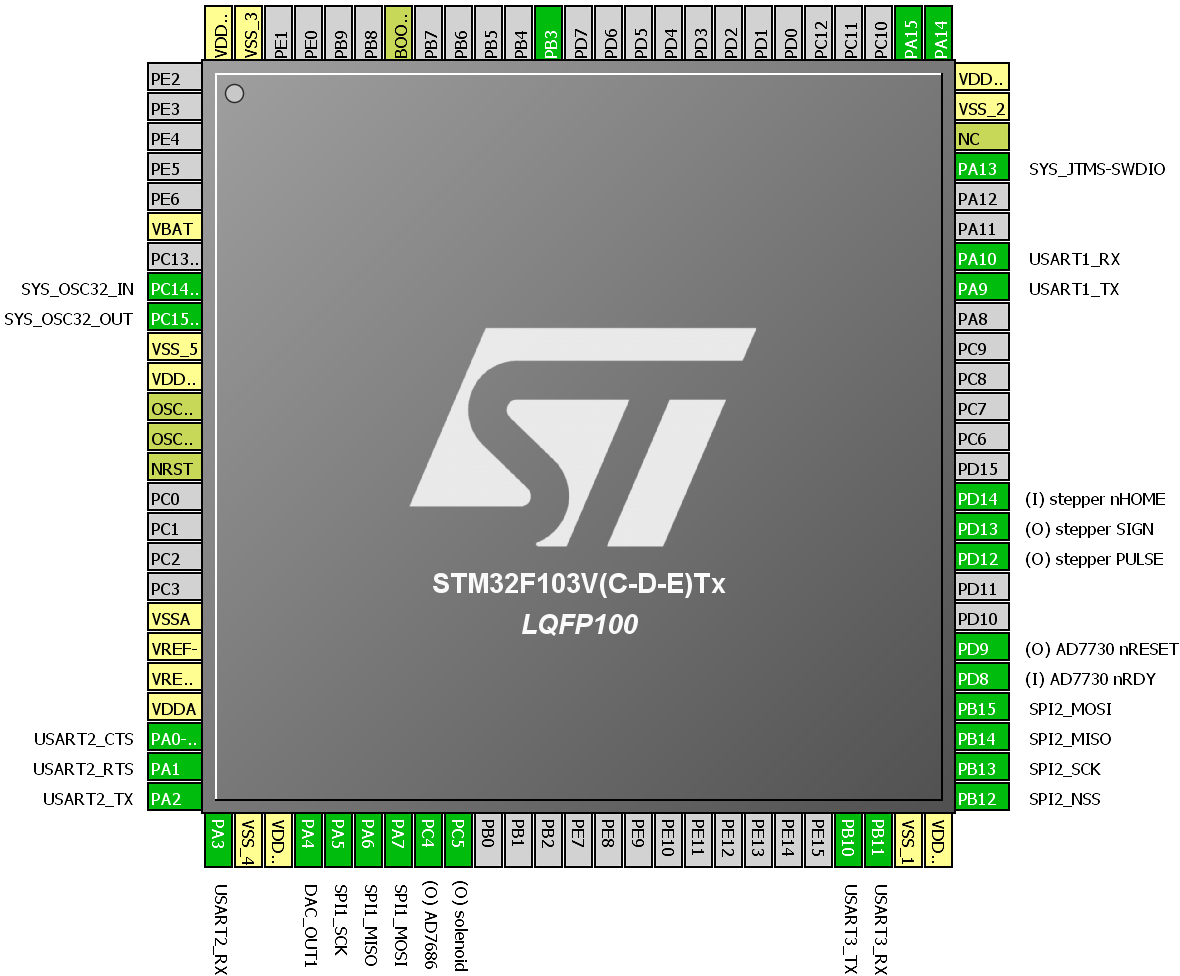
\includegraphics[width=1\linewidth]{rig/ctrl__mcu__pinout.png}
\caption{STM32F1外设与针脚资源分配图}
\label{fig:rig-ctrl-mcu-pinout}
\end{figure}

MCU的软件部分使用Keil RTX实时操作系统,系统定时器设为\SI{1}{\milli\second}周期,不同的控制过程在不同的操作系统线程(在RTX中称为``task'',即任务)中并发运行,互相可通过信号量(semaphore)、事件(event flag)等线程间通信手段实现信息传递与同步。其中:主线程负责与PC通信,接收PC传来的指令,协调其他线程,并将采集到的数据简单处理后传回PC;数据采集线程负责与AD7686与AD7730通信,协调同步采样时序;电动推杆控制线程负责向步进电机驱动器发送脉冲指令,记录电动推杆位置,实现自动回零等;DAC控制线程负责向电子比例阀输出平缓上升的斜坡信号。以下重点讨论较为复杂的数据采集与电动推杆控制部分。

\subsubsection{数据采集部分}\label{sec:rig-ctrl-mcu-adc}

在设计数据采集时序前,需先确定两ADC的采样率。AD768x系列允许的最大采样率至少为\SI{100}{\kHz},而压强变送器本身的输出更新速率为\SI{50}{\Hz},因此可以适当过采样以提高ADC有效精度。AD7730的采样率可通过SPI接口配置,最高可达\SI{1}{\kHz},且由于AD7730为$\Sigma$--$\Delta$型ADC,其采样率越低,有效精度越高。为简化实现,将两ADC的采样率均定为\SI{100}{\Hz},这样即可实现同步采样:AD7686的采样由其\bverb|CNV|引脚上升沿控制,即采样率由外部决定,而AD7730的采样率由其内部时钟与配置寄存器决定;因此可使用AD7730的中断请求引脚\bverb|nRDY|作为同步信号,触发转换与读取时序如图~\ref{fig:rig-ctrl-mcu-adc-timing}:中断响应后,立刻开始AD7686转换,并同时开始读取AD7730数据;当AD7730数据读取完毕时,AD7686转换已完成,可继续读取AD7686数据。

\begin{figure}[tbh]
\centering
\begin{minipage}{1\textwidth}
\resizebox{1\textwidth}{!}{
\begin{tikztimingtable}
  [ timing/font=\ttfamily
  , timing/slope=0.2
  , timing/coldist=12pt % column distance
  , timing/c/arrow pos=0.7
  , timing/c/arrow tip=stealth
  , xscale=0.6, yscale=1.5
  , thick
  ]
{AD7730 nRDY}  & []
  H 2L L;
  7{2L} 8{2E} 1{2H};
  H;
  32H;
  H ; [dotted] 3H; \\
{AD7730 nCS\ } & []
  H 2H L;
  32L;
  H;
  32H;
  H; [dotted]3H; \\
{AD7730 SCLK}  & [timing/c/falling arrows]
  L 2L L;
  32{C};
  L;
  32L;
  L; [dotted] 3L; \\
{AD7730 MISO}  & []
  Z 2Z Z;
  32b{1}{16-bit\footnotemark[1]{} data}{1};
  Z;
  32Z;
  Z; [dotted] 3Z; \\
\\
{AD7686 CNV\ } & []
  L 2L H;
  32H;
  L;
  32L;
  L; [dotted] 3L; \\
{AD7686 SCK\ } & [timing/c/rising arrows]
  L 2L L;
  32L;
  L;
  0C0C 32{C};
  L; [dotted] 3L; \\
{AD7686 MISO}  & []
  Z 2Z Z;
  32Z;
  0.5Z;
  32b{1}{16-bit data}{1};
  1.5Z; [dotted] 3Z; \\
\extracode
  \begin{scope}[on background layer, help lines]
    \vertlines[red, semithick]{1.1}
    \vertlines[olive, semithick]{3.2,36.0}
  \end{scope}
\end{tikztimingtable}
}

\footnotetext[1]{受各种噪声影响,预计实际有效位数略低于16位,因此将AD7730配置为16位输出。}

\end{minipage}
\caption{ADC通信时序}
\label{fig:rig-ctrl-mcu-adc-timing}
\end{figure}

\subsubsection{电动推杆控制部分}\label{sec:rig-ctrl-mcu-stepper}

由\ref{sec:rig-probe-feeding}节讨论知,电动推杆的主要作用为控制微力探头与晶圆接触。在此之前,需先将电动推杆移动到其零位,即推杆最短的位置。由于零位传感器存在一定滞回(见\ref{sec:rig-ctrl-intf-stepper}节),采用如下步骤回零:首先,若零位传感器处于未动作状态,则快速驱动电动推杆缩短,直至零位传感器动作;然后,以稍慢的速度驱动电动推杆伸长,直至零位传感器不再动作;最后,缓慢驱动电动推杆缩短,直至零位传感器再次动作;此时可认为电动推杆处于确定的零位。与电机驱动器的底层接口方面,由于电动推杆只需缓慢匀速运动,直接使用MCU内置定时器输出固定频率的脉冲即可实现。另外,为防止意外造成电动推杆超过其行程,在回零之后,需持续记录已发送的脉冲数,在预计推杆即将超过行程时停止运动。


\section{本章小结}\label{sec:rig-summary}

%TODO:summary
% !TeX root = ../main.tex
\chapter{检测平台搭建与调试}\label{ch:impl}







%-------------------------------------------------------
%                       stash
%-------------------------------------------------------


由于LSB200微力传感器安全过载仅\SI{1}{\newton},装配时应特别小心,避免对其造成不可恢复的损伤。正确的装配方法如下:

\begin{enumerate}
  \item
    将LSB200接入电控系统
    %TODO:xref AD7730
    ,并在整个装配过程中监测其读数,尽量避免其受力超过满量程。
  \item
    LSB200处于平放状态(贴有商标一面向上),轻轻握住LSB200活动端,将螺纹转接头的M3外螺纹端旋入LSB200活动端,并在保证LSB200不过载的同时,将转接头旋紧。
  \item
    用小钳子夹住转接头,将红宝石探头旋入转接头的M2内螺纹端。
  \item
    使LAC-10A/JYPY-02213处于伸长状态,轻轻握住传感器侧面(固定端),将其连接在推杆末端/平移台上。
  \item
    将LAC-10A/JYPY-02213固定在连接板上。
\end{enumerate}


由于检测平台处于试验阶段,电控系统组成随时可能发生变化,因此直接使用最小系统版作为MCU载体。
% !TeX root = exp.tex
\chapter{试验与数据分析}\label{ch:exp}

%TODO:lead-in



\section{试验方案}


%TODO: relocate
\subsection{检测流程}\label{sec:rig-overall-proc}

一次完整的检测过程分如下步骤完成:

\begin{enumerate}
  \item 准备静电卡盘
  \begin{enumerate}
    \item 用无水乙醇擦拭静电卡盘与晶圆
    \item 将晶圆小心地放置在静电卡盘陶瓷层正中央
    \item 开启静电电源,调节电极电压至目标电压
  \end{enumerate}
  
  \item 准备测量平台
  \begin{enumerate}
    \item 降下微力探头,使其轻轻接触晶圆
    \item 确认背吹控制系统中调压装置均处于零位
  \end{enumerate}
  
  \item 检测
  \begin{enumerate}
    \item 开始自动记录微力探头受力、背吹入口气压两变量
    \item 背吹气压接通并缓慢、均匀地上升
    \item 当微力探头受力即将达到其满量程时,自动切断背吹气压,检测停止
  \end{enumerate}
  
  \item 后续处理
  \begin{enumerate}
    \item 导出采集到的数据
    \item 微力探头复位上升
    \item 切断静电电源,短接两电极引线,消除部分残余电荷
    \item 小心将晶圆取下
  \end{enumerate}
\end{enumerate}
% !TeX root = ../main.tex
\cleardoublepage
\chapter{数据分析}\label{ch:analysis}

上一章的正式试验(\ref{sec:exp-main}节)中测得了\SIrange{1800}{2600}{\V}电压下的多组数据,并经初步处理得到$F$ -- $p$曲线以及关键点。本章将重点探讨这些数据所揭示出的晶圆脱附的物理过程,并据此判断出数据曲线中的晶圆脱附点,进而得到脱附背吹压强 -- 电压数据点。

\section{典型$F$ -- $p$曲线分析}\label{sec:analysis-example}
\section{曲线特征及对应物理过程}\label{sec:analysis-feature}
\section{脱附点的判定}\label{sec:analysis-criterion}
\section{数据汇总与拟合}\label{sec:analysis-tally}
\section{本章小结}\label{sec:analysis-summary}
% !TeX root = ../main.tex
\cleardoublepage
\chapter{结论}\label{ch:conclusion}


\section{论文的主要工作和创新}\label{sec:conclusion-review}

本文通过对已有静电卡盘静电力检测方案的分析,找出了其中存在的影响其检测准确度与可重复性的问题,并针对这些问题提出了改进思路,形成了改进的静电力检测方案。依据改进方案,本文设计了完整的大气条件下的静电力检测平台(可推广至真空条件),并将其实际搭建出来,经过初步试验,确定了使用该平台检测静电力的方法、流程与注意事项,将其应用于正式试验中,得到了大量能够反映静电卡盘静电吸附特性的数据,成功验证了检测方案以及平台设计能够较为准确地检测静电力。本研究主要的创新点如下:

\begin{enumerate}
  \item 提出在已有的背吹平衡法检测静电力的方案中,气隙在晶圆脱附过程中的扩大以及背吹气体的稳态流动与等效作用面积对检测的准确性产生的影响。针对气隙影响,提出了微力探头这一新检测思路,既能控制、消除气隙扩大的影响,又能更加准确地判断脱附,还部分揭示出了晶圆脱附过程的复杂性。针对背吹气体,提出了重力平衡法这一思路,可作为进一步探究晶圆受背吹作用提供借鉴。
  \item
  晶圆脱附过程的复杂性实际上推翻了已有研究中对其作出的多种假设(如静电力一定随间隙增加而降低、背吹气层在晶圆下表面的压强为均匀分布等),为相关研究指出了可能的新方向。
  \item 已有的静电力检测方案受其环境影响,费时费力;本文提出的检测方案直接在大气下工作,且检测流程中大部分操作已实现电控与自动化,可在较短时间内获得大量有效数据,不仅提高了检测的精确度,还为今后对静电力产生与消除机理的研究提供了数据基础。
\end{enumerate}


\section{工作展望}\label{sec:conclusion-future}

由于时间、条件所限,本研究中提出的方案未能全部付诸实践。首先,如\ref{sec:exp-main-proc}节所述,试验条件仍有较大的改进的余地,若能全部实现,预计试验的可重复性与准确度均会有较大提升。检测方案中的重力平衡法未能实际实现,其主要原因是因为发现“压强作用等效面积”在复杂的脱附过程中可能并非常量,而可能是与具体的脱附过程有关,导致标定该量失去意义。检测平台中的背吹控制系统仍不完善,现在完全依靠机械式减压阀来供压,应在未来的工作中,选用更合适的电子比例阀或压力控制器,甚至实现反馈控制泵式压力控制器等,以实现背吹供压的自动化。另外,由于本研究带有探索性质,电控系统未能实现更高的集成度,目前仍是较多模块松散连接的方式,可以考虑在检测平台定性之后,按照本文中的原理方案,改进电控系统的具体设计与实现。




%%% 其它部分
\backmatter

% 本科生要这几个索引,研究生不要。选择性留下。
\makeatletter
\ifthu@bachelor
  % 插图索引
  \listoffigures
  % 表格索引
  \listoftables
  % 公式索引
  %\listofequations
\fi
\makeatother


% 参考文献
\bibliographystyle{thubib}
\bibliography{ref/refs}


% 致谢
%%% Local Variables:
%%% mode: latex
%%% TeX-master: "../main"
%%% End:

\begin{ack}
\end{ack}


% 附录
\begin{appendix}
% !TeX root = ../main.tex
\cleardoublepage

%%% translation-related manual formatting
\newcommand{\apptitle}[1]{\parbox{0.9\linewidth}{\centering #1}\par\bigskip}
\newcommand{\appfigref}[2]{图~#1 -- #2~}
\newcommand{\appcite}[1]{\par\bigskip\apptitle{原文索引}\noindent\parbox{1\linewidth}{\small #1}}
\chapter{外文资料的书面翻译}

\apptitle{感性耦合等离子体环境下的静电卡盘特性瞬态分析}

\noindent 摘要:本文分析了感性耦合等离子体(ICP)环境下,用于在半导体工艺过程中夹持硅晶圆的J-R型静电卡盘(ESC)。我们提出了一个静电卡盘的双层等效电路模型,其组成为一较厚的整体层和一较薄的界面层。通过测量有/无晶圆时静电卡盘的伏安特性,可算出各层的等效电阻值,以及界面层两端等效电压。在静电卡盘上施加一斜坡电压信号,并测量其瞬态电流,积分即可得到界面层等效电容中储存的电荷量。另外,我们通过缓慢降低电压而使晶圆在氦气背吹作用下脱离卡盘的方式,在原位测量出了静电卡盘施加的静电力。用我们提出的等效电路模型预测的静电力与实际测量出的静电力相吻合。

\par\bigskip

\noindent \textbf{关键词:}J-R型;静电卡盘;感性耦合等离子体;双层模型

\par\bigskip

在有等离子体参与的半导体制程中,静电卡盘广泛用于真空环境中夹持硅晶圆。常用的静电卡盘分两种:库仑型[1-3],特点是使用绝缘体电介质层(体积电阻率$\rho > \SI{1e14}{\ohm\cm}$);以及Johnsen-Rahbek(J-R)型,特点是使用半导体电介质层($\rho = \SIrange{1e10}{1e12}{\ohm\cm}$)。静电吸附力由晶圆与静电卡盘中电极在高压作用下产生的异号电荷相吸引产生。与库仑型相比,J-R型静电卡盘可在较低电压下产生较强的吸引力,其原因主要是介电层表面微观不平度与晶圆接触后,缝隙间产生强电场。但J-R型静电卡盘吸附机理较复杂,且对界面层中的很多物理参数敏感,如电导率,表面微观不平度(亚显微级),甚至电极/晶圆的宏观平面度等;并且,使用J-R型静电卡盘的工艺存在一系列问题,如残余电荷带来的较差的可重复性,静态电流造成的晶圆表面镀膜破坏,以及将晶圆从静电卡盘表面卸下时,由顶针和残余电荷作用产生的晶片破损等。

为了能够消除这些缺点,我们需要增进对J-R型静电卡盘的理解,尤其是在等离子存在的实际工况下。在之前发表的文献[6]中,我们提出了射频偏压对低密度容性耦合等离子体(CCP)条件下的静电卡盘的伏安特性的影响。这里我们提出在高密度感性耦合等离子体(ICP)条件下的瞬态分析。接通电压时的瞬态电流的积分即为界面层电荷量,缓慢关断电压时,通过检测氦气背吹流量变化可测出静电吸附力。我们提出的双层等效电路模型可解释J-R型静电卡盘的特性。

实验使用一套ICP反应腔室[7],其圆柱形不锈钢制腔室中,使用\SI{13.56}{\MHz}射频放电激发\SI{0.1}{\torr}压强下的\ce{Ar}产生等离子体。在腔室内装有一\SI{200}{\mm}直径的J-R型静电卡盘。静电卡盘的电极材料为\ce{Mo},镶嵌在\SI{5}{\mm}厚的\ce{AlN}电介质层中,与接触表面距离\SI{0.54}{\mm}。接触表面总面积为电极投影面积的60\%(直接与晶圆接触的是静电卡盘表面上的凸台,高\SI{50}{\um},长宽\SI{2}{\mm},主要作用是为氦气冷却提供通道)。

\begin{figure}[tbhp]
\centering
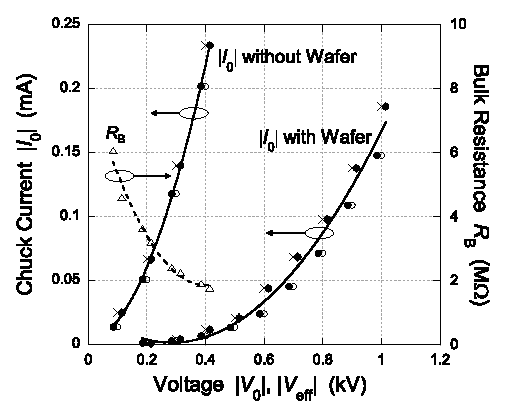
\includegraphics[width=0.7\linewidth]{_a/nagoya__1}
\caption*{图~A -- 1\hspace{1em}在有/无晶圆时,$I_0$与$\left|V_0\right|$的关系,以及无晶圆时$R_{\mathrm{B}}$的大小}
\end{figure}

首先,我们测量了\SI{600}{\W}放电,\SI{0.1}{\torr}压强产生的\ce{Ar}等离子体条件下,通过静电卡盘流向一直径\SI{200}{\mm}的硅晶圆的电流$I_0$与静电卡盘电压$V_0$(\SI{-1}{\kV}到\SI{+1}{\kV}之间)的函数关系。如\appfigref{A}{1}中``$\circ$''与``$\times$''所示,电压绝对值相同时,电流绝对值$\left|I_0\right|$在电压为负值时比电压为正值时要大。这个现象可用自偏压现象(self-bias effect)解释[6]:晶圆表面在ICP作用下,具有表面电势$V_{\mathrm{W}} \sim \SI{12}{\V}$,因此实际上静电卡盘中电极与晶圆之间的有效电压为$V_{\mathrm{eff}} = V_0 - V_{\mathrm{W}}$;即,$\left|V_0\right|$相等时,$-\left|V_0\right|$对应的有效电压更大。\appfigref{A}{1}中``$\cdot$''即为将电压修正为$V_{\mathrm{eff}}$的结果。$V_{\mathrm{eff}}/I_0$即为总电阻$R_{\mathrm{T}}$,由\ce{AlB}整体区电阻$R_{\mathrm{B}}$和接触电阻组成。%
当$\left|V_0\right|=\SI{0.4}{\kV}$时,$R_{\mathrm{T}} \sim \SI{40}{\Mohm}$;%
当$\left|V_0\right|=\SI{0.7}{\kV}$时,$R_{\mathrm{T}} \sim \SI{10}{\Mohm}$;%
当$\left|V_0\right|=\SI{1.0}{\kV}$时,$R_{\mathrm{T}} \sim \SI{6}{\Mohm}$;%
但这些数值明显大于通过体积电阻率估计出的整体层电阻$R_{\mathrm{B}} \sim \SI{3}{\Mohm}$(设$\rho=\SI{2e10}{\ohm\cm}$)。

通过测量观察到的在低电压下的高总电阻值说明在晶圆与静电卡盘中间存在较大的接触电阻。为了测出该接触电阻,首先要测量整体层电阻。将静电卡盘表面直接暴露在等离子体下,不加晶圆,测得其伏安特性如\appfigref{A}{1}。由于等离子体与静电卡盘接触较好,低电压下测得的电流较高。此时,整体层电阻即为$R_{\mathrm{B}}=\left|V_{\mathrm{eff}}\right| / \left|I_0\right|$,在\appfigref{A}{1}中用``$\Delta$''表示,可达\SI{2}{\Mohm}($V_0 > \SI{0.2}{\kV}$)。随着电压降低,仍可观测到电阻升高,这可能是由于静电卡盘与等离子体中仍存在的接触电阻升高造成的。

\begin{figure}[tbhp]
\centering
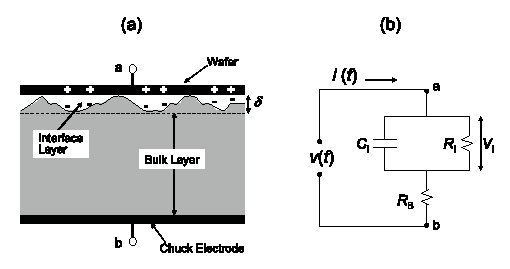
\includegraphics[width=0.7\linewidth]{_a/nagoya__2}
\caption*{图~A -- 2\hspace{1em}(a)\ J-R型静电卡盘双层模型\quad (b)\ 其等效电路}
\end{figure}

由\appfigref{A}{1}所示的测量数据,总结出\appfigref{A}{2}所示的J-R型静电卡盘双层模型,及其等效电路模型(\appfigref{A}{2(b)})。可将电极与晶圆之间的\ce{AlN}分为厚度$l=\SI{0.54}{\mm}$的整体层,其电阻为$R_{\mathrm{B}}$;以及厚度为$\delta$,较薄的界面层,其电阻为$R_{\mathrm{I}}$,电容为$C_{\mathrm{I}}=\varepsilon_0 S_{\mathrm{I}} / \delta$($S_{\mathrm{I}}$为待定的电容等效面积)。由于$\delta \ll l$,整体层的电容可忽略。总电阻$R_{\mathrm{T}}=R_{\mathrm{B}}+R_{\mathrm{I}}$。由伏安特性可知,$R_{\mathrm{I}}$随有效电压$V_{\mathrm{eff}}$非线性变化;这是J-R效应影响造成的,其机理可归结为在强电场下的电子场致发射现象[7,9,10]。整体层中流过的电流分布较均匀,但在通过界面层的若干个不规则接触点时,产生不均匀分布,并在接触点附近留下表面电荷$Q_0$;这样,晶圆与静电卡盘上的异号电荷形成了真空中的分布电容,其平均间隙为$\delta$;静电吸附力由此产生。随时间丢失的电荷由静态电流$I_0$补充,因此有如下稳态方程:
\begin{equation}\tag*{(A-1)}\label{eq:-a-1}
V_{\mathrm{I}}=R_{\mathrm{I}} I_0
Q_0=C_{\mathrm{I}} V_{\mathrm{I}}
\end{equation}

\begin{figure}[tbhp]
\centering
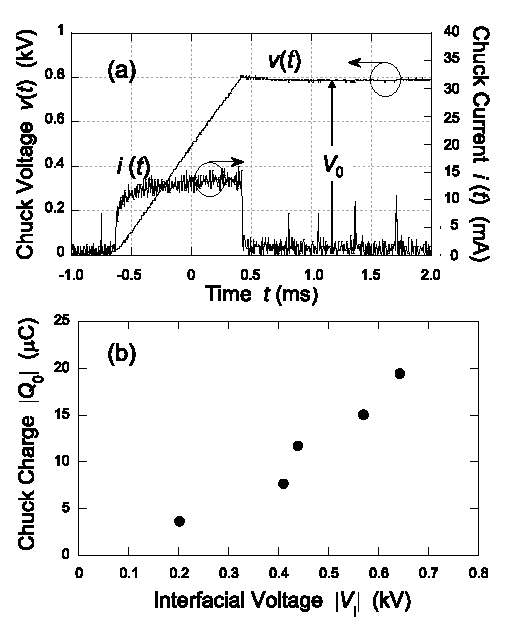
\includegraphics[width=0.5\linewidth]{_a/nagoya__3}
\caption*{图~A -- 3\hspace{1em}(a)\ $v(t)$与$i(t)$随时间变化\quad (b)\ 卡盘电荷$\left|Q_0\right|$随界面层电压$V_{\mathrm{I}}$变化关系 (\SI{600}{\W}、\SI{0.1}{\torr}条件下)}
\end{figure}

\begin{figure}[tbhp]
\centering
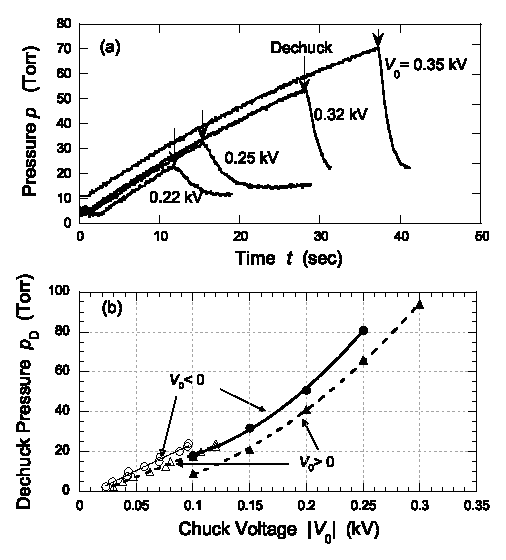
\includegraphics[width=0.5\linewidth]{_a/nagoya__4}
\caption*{图~A -- 4\hspace{1em}(a)\ 流量为\SI{10}{\sccm},电压不同时的氦气压强随时间变化关系\quad (b)\ 脱附压强随电压关系,负$V_0$为圆形点,正$V_0$为三角形点,恒流量法为实心点,恒压强法为空心点}
\end{figure}

为了得到稳态电荷$Q_0$,可在静电卡盘上施加一斜坡电压信号,并测量流过静电卡盘的瞬态电流,如\appfigref{A}{3(a)},电压$V_0$在$\tau_{\mathrm{R}} \sim \SI{1}{\ms}$内从0线性上升到\SI{0.8}{\kV}。电压关断时测得结果与接通时基本相同,只是电流方向相反(未在图中画出)。在图中,$\SI{-0.4}{\ms}<t<\SI{+0.4}{\ms}$时,可观测到较大(\SI{13}{\mA})的充电电流,之后迅速降到很小的稳态电流值(\SI{0.08}{\mA});偶尔出现的电流尖峰可能是由限流元件产生的。将测得的瞬态充电电流积分即可得到静电卡盘表面电荷量$Q_0$。如此可测得各电压$V_0$($<0$)下的表面电荷数据。定义界面层电压$V_{\mathrm{I}} = V_{\mathrm{eff}} - R_{\mathrm{B}} I_0$(即等效电路图中$C_{\mathrm{I}}$与$R_{\mathrm{I}}$两端的电压),其与$Q_0$关系如\appfigref{A}{3(b)}。可见,电荷量与电压并不成正比,其等效电容$C_{\mathrm{I}} = \left|Q_0\right| / \left|V_{\mathrm{I}}\right|$,在电容两端电压%
为\SI{0.2}{\kV}时为\SI{18}{\nano\farad},%
在\SI{0.64}{\kV}时为\SI{30}{\nano\farad}。%
这种电容随电压上升的现象,我们暂时认为是由于电压升高导致静电力升高,使得界面层厚度$\delta$缩小造成的。

通过原子力显微镜测量得到硅晶圆的表面粗糙度为\SIrange{0.8}{1.6}{\um}。考虑到介电层表面与晶圆表面的微观与宏观不平度,我们估计在电压为\SI{0.2}{\kV}时,界面层平均厚度$\delta \sim \SI{5}{\um}$;此时$C_{\mathrm{I}}=\SI{18}{\nano\farad}$,得到电容等效面积$S_{\mathrm{I}} \sim \SI{1.02e-2}{\m^2}$。另外,由于表面凸台影响,介电层与晶圆的实际接触面积为\SI{200}{\mm}直径圆形晶圆的60\%\footnotemark{},即$S_*=\SI{1.88e-2}{\m^2}$。

\footnotetext{译者注:此处原文意为“减小60\%接触面积”,有误,根据前后数据推断,实际应为“接触面积为整个晶圆的60\%”。}

为了检测静电吸引力,我们将一定压强的氦气通入晶圆与静电卡盘之间的空隙中。当作用在晶圆上的气体向上的压力稍微超过静电吸附力时,晶圆将脱离静电卡盘表面;此时氦气压力和/或流量将会发生改变。我们采用了两种测量方式:恒流量法和恒压强法。

如\appfigref{A}{4(a)},恒流量法是将氦气以固定的质量流量(\SI{10}{\sccm},即标况下\SI{10}{\cm^3\per\s})通入静电卡盘;共测试了4组电压下的情况:\SIlist[list-separator={,},list-final-separator={,以及}]{0.22;0.25;0.32;0.35}{\kV}。随着氦气流入,其压强逐渐升高;晶圆脱离后,由于气体大量漏出,压强突然降低。因此,图中标出的压强最高值,即晶圆即将脱离时的压强$p_{\mathrm{D}}$,就是气压与静电力平衡时的压强。\appfigref{A}{4(b)}中``$\bullet$''与``$\Delta$''分别表示$V_0 < 0$与$V_0 > 0$时,$p_{\mathrm{D}}$与$\left|V_0\right|$的关系。可见$V_0 < 0$时,吸附力更大。图中实线与虚线分别是两组数据的拟合曲线;其距离大约是\SI{25}{\V},与$V_{\mathrm{W}}$二倍大致相当,符合之前由\appfigref{A}{1}得出的结论。

在一系列试验过程中,我们发现前一次实验的结果会严重影响后一次,其原因为:当晶圆脱离后,在静电卡盘表面仍残留部分表面电荷,而这些电荷会影响后续试验。为了保证试验可重复性,我们在晶圆脱离后,将脱离的晶圆移至真空交换室(load-lock chamber),然后将静电卡盘暴露在\SI{0.1}{\torr}压强的\ce{Ar}等离子体中\SI{30}{\s},以去掉其表面残余电荷;这样即可保证采集数据可靠性。

\begin{figure}[tbhp]
\centering
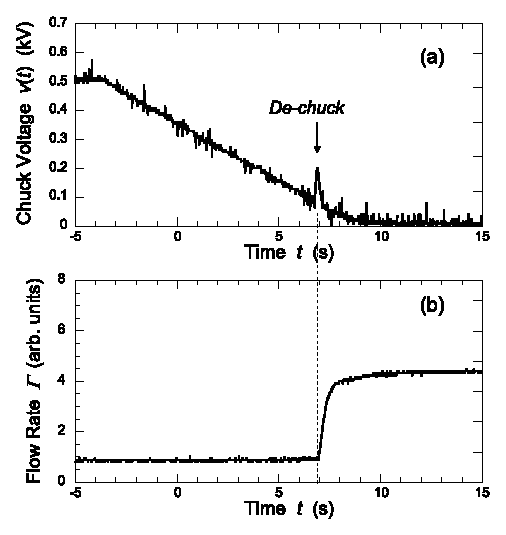
\includegraphics[width=0.7\linewidth]{_a/nagoya__5}
\caption*{图~A -- 5\hspace{1em}(a)\ $v(t)$随时间变化\quad (b)\ 氦气流量$\Gamma$随时间变化}
\end{figure}

在电压较低($\left|V_0\right| < \SI{0.15}{\kV}$)时,由于信号较小,而扰动较大,恒流量法测试精度下降。因此,在低电压区我们改用恒压强法来检测静电力。如\appfigref{A}{5},在维持氦气压力一定时,缓慢降低静电卡盘电压。氦气压强维持在$p = \SI{10}{\torr}$时,电压$V_0$在$t=\SI{-3.5}{\s}$时开始由\SI{0.5}{\kV}缓慢下降(约需10 s降至\SI{0}{\V})。\appfigref{A}{5(b)}中可见,在$t=\SI{7}{\s}$时,氦气流量突然增加,说明此时晶圆脱离,对应电压为\SI{0.07}{\kV}。脱离后,氦气流量迅速达到流量控制器允许的最大流量(\SI{50}{\sccm})。另外,在脱离时,可观测到电压值也出现一个尖峰,这是阻抗发生变化造成的。

当设置氦气恒定压强高于\SI{10}{\torr}时,晶片更早脱离,说明脱离时静电卡盘电压更大。反复试验即可得到气压与电压的函数关系,如\appfigref{A}{4(b)}中``$\circ$''和``$\Delta$''所示。当$\left|V_0\right|=\SI{0.1}{\kV}$时,更准确的恒定压强法获得的$p_{\mathrm{D}} \sim \SI{20}{\torr}$,约是恒流量法测试结果的两倍。

气体压强作用在晶圆上的面积$S_{\mathrm{M}}=\SI{1.26e-2}{\m^2}$(\SI{200}{\mm}直径晶圆的40\%)\textit{,除了电容等效面积$S_{\mathrm{I}}$}\footnotemark{}。因此,气压作用在晶圆上的合力为
\begin{equation}\tag*{(A-2)}\label{eq:-a-2}
F_{\mathrm{M}} = p_{\mathrm{D}} S_{\mathrm{M}}
\end{equation}
另一方面,使用测量得到的电容模型,可估计静电力为:
\begin{equation}\tag*{(A-3)}\label{eq:-a-3}
F_{\mathrm{E}} = \frac{D^2}{2 \varepsilon_0} S_{\mathrm{I}}
\end{equation}
其中电位移$D=Q_0/S_{\mathrm{I}}$。当静电卡盘电压$\left|V_0\right|=\SI{0.1}{\kV}$时,较准确的恒压强法测得$p_{\mathrm{D}} \sim \SI{20}{\torr}$,可得$F_{\mathrm{M}} \sim \SI{33.5}{\N}$;同条件下测得的表面电荷量$Q_0 \sim \SI{2.5}{\micro\coulomb}$,可得$F_{\mathrm{E}} \sim \SI{35.3}{\N}$。两者相差不大,在实验误差允许范围内,验证了晶圆脱离时$F_{\mathrm{M}}=F_{\mathrm{E}}$这一关系。

\footnotetext{译者注:原文此处语法不通,且由后面计算推断,此处并未从$S_{\mathrm{M}}$中扣除$S_{\mathrm{I}}$。}

总结:我们分析了ICP反应腔室中J-R型静电卡盘的基本特性,提出了由较厚阻性层与较薄容性层构成的双层电路模型,并通过加/不加晶圆的方法,用伏安特性法测量出了每一层的电阻值。加电压时的瞬态测量提供了一种新的测量静电卡盘表面电荷量的方式,并间接提供了估计静电力的方式(静电力与电荷量平方成正比)。我们还提出了一种利用氦气加压的较为精确地在原位测量静电力的方式;该法测量出的静电力与等效电路模型估测出的静电力相符较好。

\appcite{[1] SHIM G. I., SUGAI H. Temporal Analysis of Electrostatic Chuck Characteristics in Inductively Coupled Plasma[J]. Plasma and Fusion Research, 2008, 3: 028-028.} 


\clearpage


\apptitle{对夹持硅晶圆用的静电卡盘的基础研究}

\noindent 摘要:在半导体工业中,机械夹持晶圆的装置可能导致严重的问题。改用静电卡盘是可能解决这些问题的一种途径。我们研究了由交错电极和薄膜介电层组成的静电卡盘对硅片产生的静电吸引力的规律。当电压上升或介电层厚度降低时,静电力均上升。当交错电极的宽度和间距降低时,也能获得更强的静电力。实验表明当电极宽度和间距均为\SI{1}{\mm}、介电层为\SI{50}{\um}时,可获得最强的静电力:电压3.7 kV、吸引4英寸晶圆时,竖直方向静电力约为\SI{17}{\N}。在施加高压直流电压后,即使撤去电压,仍存在一些残余静电力,这种效应可用施加变频交流高压电的方式解决。

\par\bigskip

\noindent \textbf{关键词:}薄膜介电层;静电卡盘;静电力;硅晶圆夹持;交错电极

\par\bigskip

在半导体工业中,光学成像、化学气相沉积(CVD)、以及干法刻蚀等系统工作在真空条件下,而因为此时不能使用真空吸盘,机械夹持系统被广泛应用。但在搬运和夹持过程中,机械夹持系统对晶圆造成的污染可能会造成严重的问题。除此之外,机械夹持作用于晶圆的边缘处,因此可能无法保证其平整度。基于静电的夹持系统可能是一种解决这些问题的方法[1,2]。静电卡盘(ESC)可以在晶圆上施加分布夹紧力,足以使晶圆平整。另外,由于机械夹持系统在搬运时,为了避免颗粒污染,不能快速运动,而静电卡盘则无此问题,可以更快地搬运晶圆,提高产率。

虽然静电卡盘已经在坐标记录仪中应用了数十年[3],直到1970年代才由Wardly[4]提出可将其用于夹持硅晶圆。从此,因为上文所述的优点,大量半导体工业研究者开始投入到静电卡盘的研究中。这些研究的结果多数为专利;相比之下,学术刊物中出现的论文相对较少。

已经提出的静电卡盘种类很多[5],但基本上可分为两类:第一类静电卡盘需要将硅晶圆自身连接到高压电源上,称为“平行板电容器”(PPC,parallel-plate capacitor)型静电卡盘;第二类静电卡盘不需要硅晶圆与电源有电气连接,而是将电源连接到埋藏在介电层中的两个电极上,称为“交错电极”(IDE, interdigitated electrodes)型静电卡盘。在金属电极和硅晶片中间必须要有一层绝缘材料才能使其正常工作。

一般认为交错电极型静电卡盘产生的静电力要比平行板电容器型要弱,但交错电极型具有无需硅晶圆与电源有电气连接的优点,可大大简化整个系统。因此,我们选择交错电极型静电卡盘作为对象,通过改变其参数,以求获得尽可能强的静电力,来研究其基本特性。

\begin{figure}[tbhp]
\centering
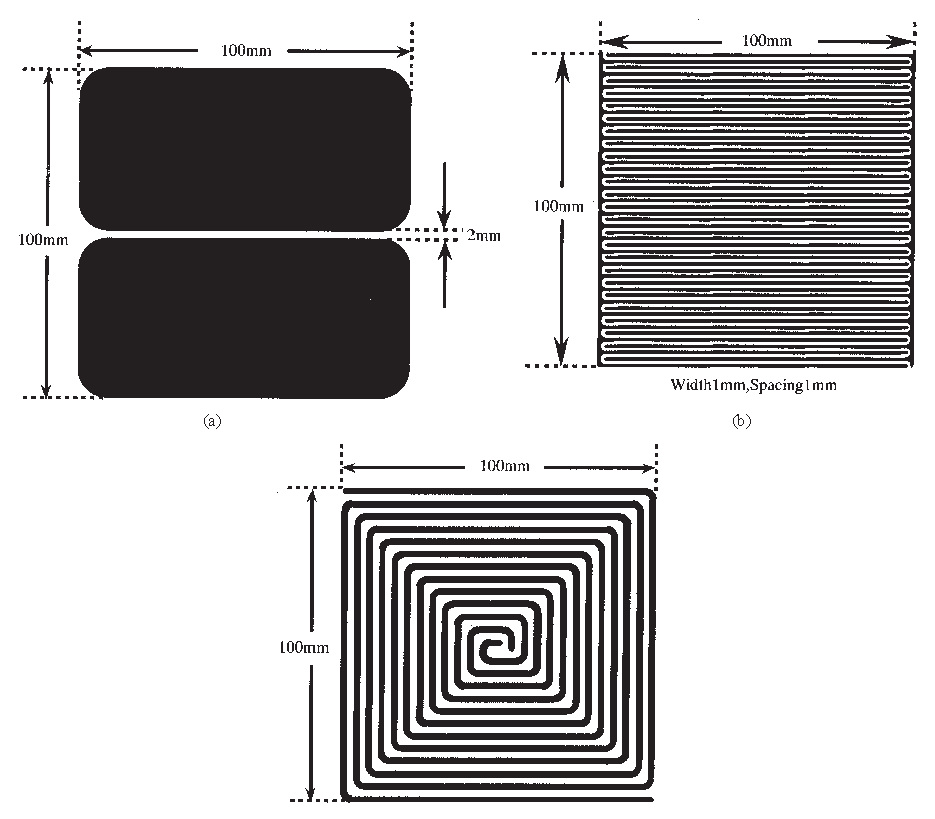
\includegraphics[width=0.7\linewidth]{_a/asano__1}
\caption*{图~A -- 6\hspace{1em}电极布置\quad (a)共平面型\quad (b)\ 平行交错\quad (c)\ 螺旋交错}
\end{figure}

\begin{figure}[tbhp]
\centering
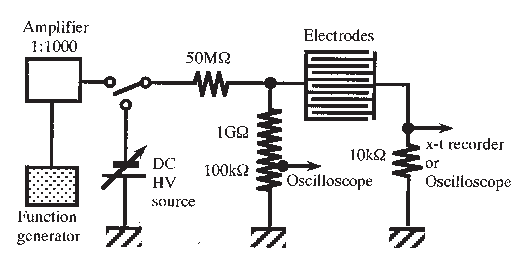
\includegraphics[width=0.7\linewidth]{_a/asano__2}
\caption*{图~A -- 7\hspace{1em}测量系统}
\end{figure}

\begin{figure}[tbhp]
\centering
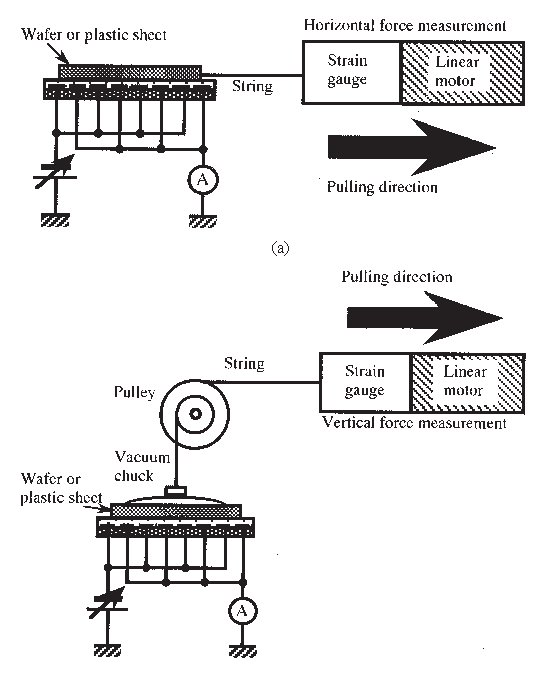
\includegraphics[width=0.7\linewidth]{_a/asano__3}
\caption*{图~A -- 8\hspace{1em}测力系统\quad (a)横向阻力\quad (b)\ 纵向吸引力}
\end{figure}

\begin{figure}[tbhp]
\centering
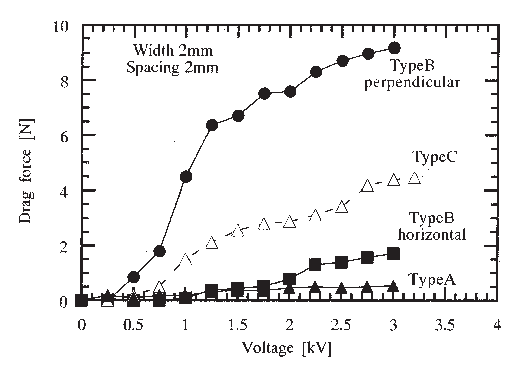
\includegraphics[width=0.7\linewidth]{_a/asano__4}
\caption*{图~A -- 9\hspace{1em}不同电极布置与牵引方向对力与电压关系的影响}
\end{figure}

\begin{figure}[tbhp]
\centering
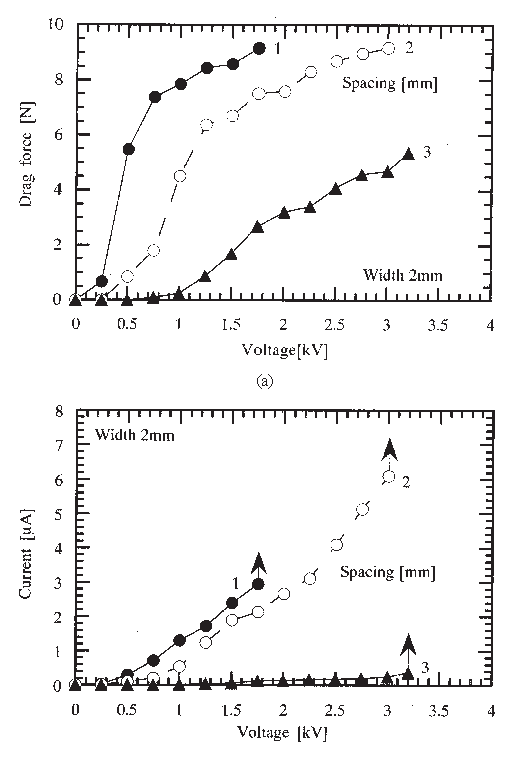
\includegraphics[width=0.7\linewidth]{_a/asano__5}
\caption*{图~A -- 10\hspace{1em}随电极间距的变化关系:\quad (a)\ 力\quad (b)\ 电流}
\end{figure}

\begin{figure}[tbhp]
\centering
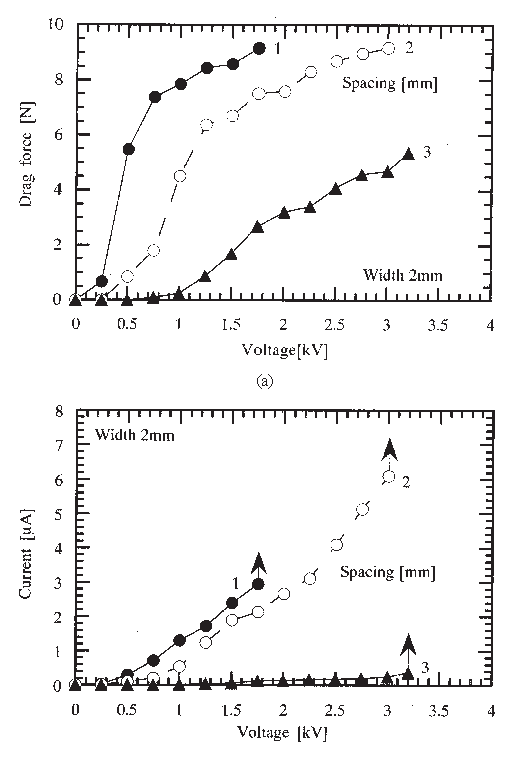
\includegraphics[width=0.7\linewidth]{_a/asano__5}
\caption*{图~A -- 10\hspace{1em}随电极间距的变化关系:\quad (a)\ 力\quad (b)\ 电流}
\end{figure}

\begin{figure}[tbhp]
\centering
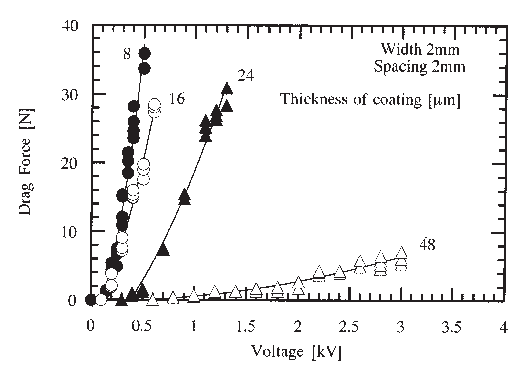
\includegraphics[width=0.7\linewidth]{_a/asano__6}
\caption*{图~A -- 11\hspace{1em} 横向阻力随电压与绝缘薄膜厚度关系}
\end{figure}

我们测试了很多电极布置,其中部分如\appfigref{A}{6}:\appfigref{A}{6(a)}为共平面电极,下文简称A型;(b)与(c)为不同形状的交错电极,使用印刷电路板(PCB)工艺制成,下文分别简称B、C型。由于我们希望研究静电卡盘的基本特性,试验在大气条件下进行\footnotemark{}。在前期试验中,我们用一张透明幻灯片代替硅晶圆。当使用一张4英寸的硅晶圆做实验时,在晶圆与电极之间插入另一种塑料薄片,用于调节晶圆与电极之间的距离。

\footnotetext{译者注:逻辑不明但原文如此。}

测量系统如\appfigref{A}{7},可切换接通直流或交流电压,其中交流电压包括固定的\SI{50}{\Hz}以及由函数发生器经电压放大器产生的变频交流电压。静电吸引力由\appfigref{A}{8}所示系统测出。靠直接横向牵引晶圆或幻灯片可测出横向阻力,如\appfigref{A}{8(a)};在晶圆上方设置真空吸盘,用绳子通过滑轮,使用直线电机牵引,中间放置应变式力传感器,以此检测竖直方向静电吸引力。

为了探明电极方向性,我们首先横向牵引一张幻灯片。由于幻灯片的材料为PET(聚对苯二甲酸乙二酯),电极上并未覆盖额外的绝缘材料。试验中使用了不同形状参数的电极,如线宽和间距从\SI{0.5}{\mm}变化到\SI{3.0}{\mm}的B型电极。

\appfigref{A}{9}为横向阻力与电压关系,其中电极线宽与间距均为\SI{2}{\mm} mm。双共平面电极(A型)产生的阻力最小;当垂直于B型电极方向牵引时产生的阻力最大,当平行于电极方向时产生的阻力极其微弱;C型电极在各方向产生的阻力基本相等。B型电极显现出的方向性无法用简单的静电理论解释。由于B型电极产生的力高于其他两种,我们选择它作为进一步试验的对象。阻力与电极间距的关系如\appfigref{A}{10}.显然,间距越小,产生力越大;但当间距缩小至\SI{0.5}{\mm}时,试验结果并不理想,这可能是受到电极制造工艺的限制。因此,我们将间距与宽度均为\SI{1}{\mm}的B型电极选为试验基准。

由\appfigref{A}{10(b)}可看出,当电压增加至击穿时,电流迅速增加,为了防止击穿,增加静电吸引力,在电极上喷涂一层绝缘涂料(光刻胶GR-303);使用电容法测量其厚度为约\SI{8}{\um}。之后,又测量了阻力与喷涂的绝缘层厚度的关系,如\appfigref{A}{11};可看出绝缘层越薄,力越强。

\begin{figure}[tbhp]
\centering
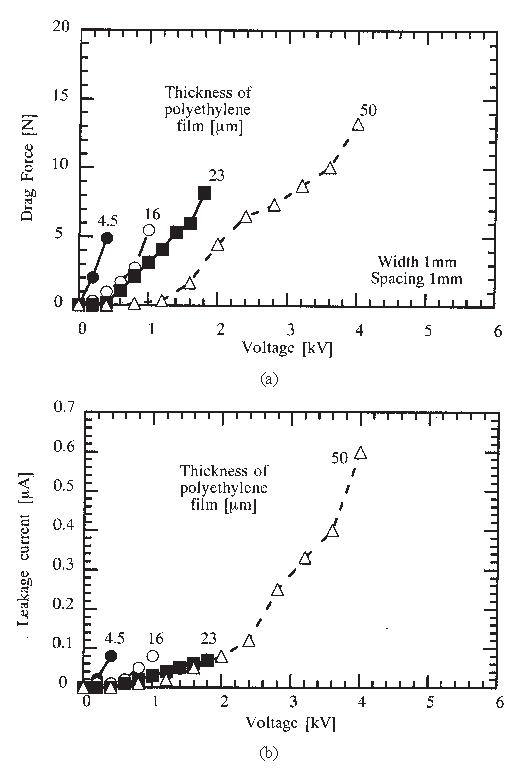
\includegraphics[width=0.7\linewidth]{_a/asano__7}
\caption*{图~A -- 12\hspace{1em} 随PE薄膜厚度变化关系:\quad (a)\ 横向阻力\quad (b)\ 电流}
\end{figure}

\begin{figure}[tbhp]
\centering
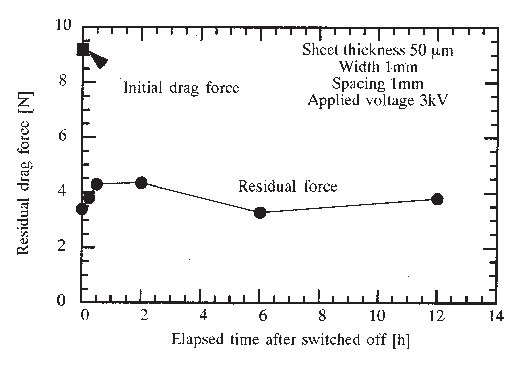
\includegraphics[width=0.7\linewidth]{_a/asano__8}
\caption*{图~A -- 13\hspace{1em} 残余静电力}
\end{figure}

\begin{figure}[tbhp]
\centering
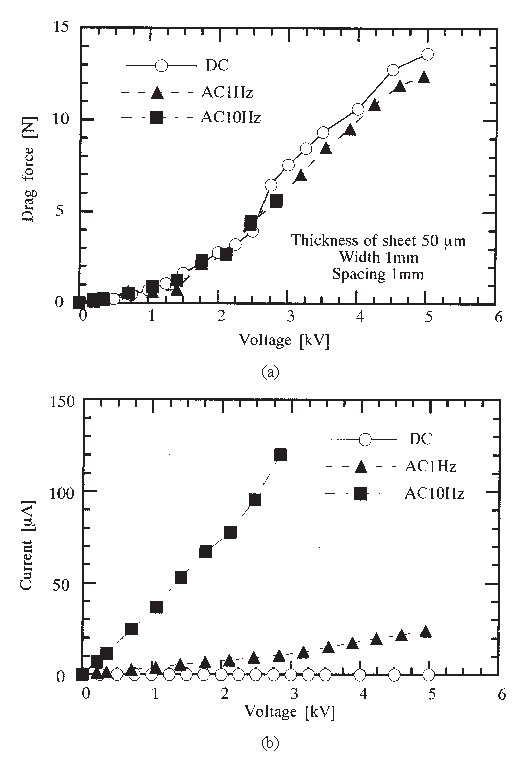
\includegraphics[width=0.7\linewidth]{_a/asano__9}
\caption*{图~A -- 14\hspace{1em} AC/DC电源对比:\quad (a)\ 力随电压变化\quad (b)\ 电流随电压变化}
\end{figure}

\begin{figure}[tbhp]
\centering
\includegraphics[width=0.7\linewidth]{_a/asano__10}
\caption*{图~A -- 15\hspace{1em} 残余静电力与电流随频率变化关系}
\end{figure}


虽然我们将多种不同材料的绝缘层放置在电极和晶圆中间测试,其中只有PE(聚乙烯)薄膜有多种厚度,因此,大量实验中使用了不同厚度的PE薄膜。由于电极是用PCB工艺刻蚀而成,在电极间存在\SI{35}{\um}高的凸台,导致在施加高压时击穿产生的气隙。因此我们使用硅胶填充这一空隙。横向阻力随电压关系如\appfigref{A}{12}。可见,当PE绝缘层厚度为\SI{50}{\um}高时,可以产生相当强的阻力;当使用更薄的绝缘层时,其表面稳定性变差,经常随晶圆一起被拖动,导致阻力降低。

在使用直流电压试验时,发现残余电荷对试验有很大影响:切断电源较长时间后仍存留有横向阻力。\appfigref{A}{13}是一次测量的结果:初始阻力为\SI{9}{\N}(电压3 kV,绝缘层厚度\SI{50}{\um}),而切断电源12小时后,仍有\SI{4}{\N}阻力残留。为了解决此问题,我们尝试使用高压交流电源。当使用\SI{50}{\Hz}交流电源时,能够消除残余阻力\footnotemark{},但因为电容反复充放电,产生较大反应电流。因此,我们使用函数发生器和电流放大器产生低频高压交流电压。\appfigref{A}{14}比较了使用直流、\SI{1}{\Hz}、\SI{10}{\Hz}电源时产生的阻力和电流大小。如\appfigref{A}{15}所示,采用低频交流供电时,残余阻力大大减小。

\footnotetext{译者注:原文中此处逻辑混乱,疑似为日文直译造成。}

\begin{figure}[tbhp]
\centering
\includegraphics[width=1\linewidth]{_a/asano__11}
\caption*{图~A -- 16\hspace{1em}  静电吸引力随直流电压变化关系:%
\quad (a)\ 介电层厚\SI{16}{\um}%
\quad (b)\ 介电层厚\SI{23}{\um}%
\quad (c)\ 介电层厚\SI{50}{\um}%
}
\end{figure}

为了测量竖直方向上的静电吸引力,使用真空吸盘来夹持晶圆;试验中需确保真空吸盘与晶圆对中。尽管采取了这样的措施,测得的吸引力散布相当大,因此对多组数据取平均值分析。如\appfigref{A}{16},测量了不同电压、不同绝缘层厚度下的吸引力大小,并在图中表示出了平均值。发现静电吸引力较强\footnotemark{}。残余吸引力仍存在,同样可用变频交流供电法消除。

\footnotetext{译者注:原文如此。}

从初期试验中可看出,交错电极型静电卡盘能在塑料薄膜上产生较大的横向阻力,且该阻力随电极间隙减小而增强。然而由于漏电流和击穿强度等因素影响,可能存在一个最优的间隙大小,在我们的试验中得出该大小为\SI{1}{\mm};该值可能与电极制造工艺有关。
当使用\SI{1}{\mm}间隙的电极时,可以在晶圆上产生大于\SI{15}{\N}的静电吸引力。通过改变绝缘层材料与厚度,可以进一步增强静电吸引力。
当电极间存在绝缘材料(包括硅胶)时,即使切断电源,仍存在残余电荷,进而产生残余静电力;可用施加变频交流电压的方式减小这一影响。

\appcite{[1] ASANO K., HATAKEYAMA F., YATSUZUKA K. Fundamental study of an electrostatic chuck for silicon wafer handling[J]. Industry Applications, IEEE Transactions on, 2002, 38(3): 840-845.}
% !TeX root = ../main.tex
\cleardoublepage
\chapter{其他有参考价值的内容}


%%% mashup

\begin{sidewaysfigure}[p]
  \centering
  \begin{minipage}{\textwidth}
    \centering
    \includegraphics
      [max size={\textwidth}{0.9\textheight}]
      {_b/mashup__feeding}
    \caption{精密直线进给机构选型表(\ref{sec:rig-probe-feeding}节)}
    \label{fig:-b-mashup-feeding}
  \end{minipage}%
  \par\bigskip
  \begin{minipage}{\textwidth}
    \centering
    \includegraphics
      [max size={\textwidth}{0.9\textheight}]
      {_b/mashup__pressure}
    \caption{压强变送器选型表(\ref{sec:rig-pressure-sensor}节)}
    \label{fig:-b-mashup-pressure}
  \end{minipage}
\end{sidewaysfigure}


%%% pcb

\begin{sidewaysfigure}[p]
\centering
\includegraphics
  [max size={\textwidth}{0.9\textheight}]
  {_b/pcb__pressure}
\caption{背吹控制系统接口PCB布线图(\ref{sec:impl-pcb-pressure}节)}
\label{fig:-b-pcb-pressure}
\end{sidewaysfigure}

\begin{figure}[p]
\centering
\includegraphics
  [max size={\textwidth}{0.9\textheight}]
  {_b/pcb__ad7730}
\caption{微力传感器接口PCB布线图(\ref{sec:impl-pcb-ad7730}节)}
\label{fig:-b-pcb-ad7730}
\end{figure}

\begin{figure}[p]
\centering
\includegraphics
  [max size={\textwidth}{0.9\textheight}]
  {_b/pcb__zaber}
\caption{LAC-10A零位传感器PCB布线图(\ref{sec:impl-pcb-zaber-homing}节)}
\label{fig:-b-pcb-zaber}
\end{figure}
\end{appendix}

% 个人简历
\begin{resume}

	\resumeitem{个人简历}
	
	1991 年 10 月 11 日出生于 黑龙江 省 牡丹江 市。
	
	2010 年 9 月考入 清华 大学 机械工程 系 机械工程及自动化 专业 攻读 工学学士 学位至今。
	
	\begin{comment}
		\resumeitem{发表的学术论文} % 发表的和录用的合在一起
	
		\begin{enumerate}[{[}1{]}]
		\end{enumerate}

		\resumeitem{研究成果} % 有就写,没有就删除
		\begin{enumerate}[{[}1{]}]
		\item 任天令, 杨轶, 朱一平, 等. 硅基铁电微声学传感器畴极化区域控制和电极连接的
		方法: 中国, CN1602118A. (中国专利公开号.)
		\item Ren T L, Yang Y, Zhu Y P, et al. Piezoelectric micro acoustic sensor
		based on ferroelectric materials: USA, No.11/215, 102. (美国发明专利申请号.)
		\end{enumerate}
	\end{comment}
\end{resume}

\end{document}
